\documentclass[a4paper,12pt,fleqn,twoside,openany]{memoir} 	% Openright aabner kapitler paa hoejresider (openany = vilkaarlig/begge)

%%%% MANUEL OPSAETNING %%%%
\newcommand{\name}{SW1A325a}                 % Skriv navnet på dig eller din gruppe her
\newcommand{\sidefod}{\name}                % Skriv hvad der skal staa til venstre i sidefoden her
%Derudover: kig under 'Taelle ord'

%%%% PAKKER %%%%

\usepackage{url}
\usepackage{svg}
\usepackage{dirtytalk}
\usepackage[ruled]{algorithm2e}
\usepackage{subcaption}

% ¤¤ Oversaettelse og tegnsaetning ¤¤ %
\usepackage[T1,OT1]{fontenc}					% Output-indkodning af tegnsaet, dvs. printede fonte og tegn (T1 = Type 1 font med support for de fleste europaeiske sprog)
\usepackage[english]{babel}					% Sproglig fremstilling af elementer (figur vs. figure, litteratur vs. bibliography osv.)
\usepackage{varioref}
\addto\extrasenglish{% page 5 of varioref's manual
  \renewcommand\reftextfaceafter{on the following page}%
  \renewcommand\reftextafter {on the next page}%
  \renewcommand\reftextfacebefore{on the previous page}%
  \renewcommand\reftextbefore {on the previous page}%
}

\usepackage{ragged2e,anyfontsize}			% Justering af elementer

%Indentation
\usepackage{parskip}										
										
% ¤¤ Figurer og tabeller (floats) ¤¤ %
\usepackage{graphicx} 						% Inkludering af eksterne billeder (JPG, PNG, PDF)
\usepackage{multirow}                		% Fletning af raekker og kolonner (\multicolumn og \multirow)
\usepackage{colortbl} 						% Farver i tabeller (fx \columncolor, \rowcolor og \cellcolor)
\usepackage[dvipsnames]{xcolor}				% Definer farver med \definecolor. Se mere: http://en.wikibooks.org/wiki/LaTeX/Colors
\usepackage{flafter}% Soerger for, at floats ikke optraeder i teksten foer deres reference
\usepackage{float}							% Muliggoer eksakt placering af floats, fx \begin{figure}[H]
\let\newfloat\relax 						% Justering mellem float-pakken og memoir
%\usepackage{eso-pic}						% Tilfoej billedekommandoer paa hver side
%\usepackage{wrapfig}						% Indsaettelse af figurer omsvoebt af tekst 
%\usepackage{multicol}         	        	% Muliggoer tekst i spalter
%\usepackage{rotating}						% Rotation af tekst med \begin{sideways}...\end{sideways}

% ¤¤ Matematik mm. ¤¤
\usepackage{amsmath,amssymb,stmaryrd} 		% Avancerede matematik-udvidelser
\usepackage{mathtools}						% Andre matematik- og tegnudvidelser
\usepackage{textcomp}                 		% Symbol-udvidelser (fx promille-tegn med \textperthousand)
\usepackage{siunitx}						% Flot og konsistent praesentation af tal og enheder med \si{enhed} og \SI{tal}{enhed}
\sisetup{output-decimal-marker = {,}}		% Opsaetning af \SI og decimalseparator
%\usepackage[version=3]{mhchem} 			% Kemi-pakke til flot og let notation af formler, fx \ce{Fe2O3}
%\usepackage{rsphrase}						% Kemi-pakke til RS-saetninger, fx \rsphrase{R1}

% ¤¤ Referencer og kilder ¤¤ %
\usepackage{lastpage}                       % Muliggoer bl.a. brug af \pageref{LastPage} kommandoen
\usepackage[english]{varioref}				% Muliggoer bl.a. krydshenvisninger med sidetal (\vref)
\usepackage{natbib}							% Udvidelse med naturvidenskabelige citationsmodeller, herunder Harvard-modellen
%\usepackage{xr}							% Referencer til eksternt dokument med \externaldocument{<NAVN>}
%\usepackage{glossaries}					% Terminologi- eller symbolliste (se mere i Lars Madsens Latex-bog)
\usepackage[font=itshape]{quoting}                      % Muliggør at indsætte citater med \begin{quoting}...\end{quoting}

% ¤¤ Misc. ¤¤ %
\usepackage{listings} % Placer kildekode i dokumentet med \begin{lstlisting}...\end{lstlisting}

\usepackage{lipsum}							% Dummy tekst med fx \lipsum[2]
\usepackage[shortlabels]{enumitem}			% Muliggoer enkelt konfiguration af lister (se \setlist nedenfor)
\usepackage{pdfpages}						% Goer det muligt at inkludere pdf-dokumenter med kommandoen \includepdf[pages={x-y}]{fil.pdf}	
\pdfoptionpdfminorversion=6					% Muliggoer inkludering af pdf-dokumenter af version 1.6 og hoejere
\pretolerance=2500 							% Justering af afstand mellem ord (hoejt tal, mindre orddeling og mere luft mellem ord)

% Kommentarer og rettelser med \fxnote. Med 'final' i stedet for 'draft' udloeser hver note en error i den faerdige rapport.
\usepackage[footnote,draft,english,silent,nomargin]{fixme}		

% Muliggør blokkommentarer med \begin{comment} ... \end{comment}
\usepackage{comment}

%%%% BRUGERDEFINEREDE INDSTILLINGER %%%%

% ¤¤ Marginer ¤¤ %
\setlrmarginsandblock{2.5cm}{2.5cm}{*}		% \setlrmarginsandblock{Indbinding}{Kant}{Ratio}
\setulmarginsandblock{2.5cm}{2.5cm}{*}		% \setulmarginsandblock{Top}{Bund}{Ratio}
\checkandfixthelayout 						% Oversaetter vaerdier til brug for andre pakker

%	¤¤ Afsnitsformatering ¤¤ %
\setlength{\parindent}{0mm}           		% Stoerrelse af indryk
\setlength{\parskip}{3mm}          			% Afstand mellem afsnit ved brug af double Enter
\linespread{1,3}							% Linjeafstand

% ¤¤ Litteraturlisten ¤¤ %
\bibpunct[,]{(}{)}{;}{a}{,}{,} 				% Definerer parametre ved Harvard-henvisning (bl.a. parantestype og seperatortegn)
\bibliographystyle{0_bibtex/harvard}		% Udseende af litteraturlisten (Harvard-metoden - skift til fx 'plain' for tal)

% ¤¤ Dybde af overskrifter ¤¤ %
\setsecnumdepth{subsubsection}		 			% Dybden af nummerede overkrifter (part/chapter/section/subsection)
\settocdepth{subsection} 					% Dybden af overskrifter vist i indholdsfortegnelsen

% ¤¤ Lister ¤¤ %
\setlist{
  topsep=0pt,								% Vertikal afstand mellem tekst og listen
  itemsep=-1ex,								% Vertikal afstand mellem items
} 

% ¤¤ Visuelle referencer ¤¤ %
\usepackage[colorlinks]{hyperref}			% Danner klikbare referencer (hyperlinks) i dokumentet
\hypersetup{colorlinks = true,				% Opsaetning af farvede hyperlinks (interne links, citeringer og URL)
    linkcolor = black,
    citecolor = black,
    urlcolor = black
}

% ¤¤ Opsaetning af figur- og tabeltekst ¤¤ %
\captionnamefont{\small\bfseries\itshape}	% Opsaetning af tekstdelen ('Figur' eller 'Tabel')
\captiontitlefont{\small}					% Opsaetning af nummerering
\captiondelim{. }							% Seperator mellem nummerering og figurtekst
\captionstyle{\centering}					% Justering/placering af figurteksten (centreret = \centering, venstrejusteret = \raggedright)
\captionwidth{\linewidth}					% Bredden af figurteksten
\hangcaption								% Venstrejusterer fler-linjers figurtekst under hinanden
\setlength{\belowcaptionskip}{0pt}			% Afstand under figurteksten
		
% ¤¤ Opsaetning af listings ¤¤ %
\renewcommand{\lstlistingname}{Snippet} % Listing -> Snippet
\definecolor{commentGreen}{RGB}{34,139,24}
\definecolor{stringPurple}{RGB}{208,76,239}
\definecolor{dkgreen}{rgb}{0,0.6,0}
\definecolor{gray}{rgb}{0.5,0.5,0.5}
\definecolor{mauve}{rgb}{0.58,0,0.82}
\definecolor{light-gray}{gray}{0.25}
\definecolor{lighter-gray}{RGB}{240,240,240}

\lstset{language=C,					% Sprog
	basicstyle=\ttfamily\scriptsize,		% Opsaetning af teksten
	keywords={for,if,while,else,elseif,		% Noegleord at fremhaeve
			  end,break,return,case,
			  switch,function,free},
	keywordstyle=\color{blue},				% Opsaetning af noegleord
	commentstyle=\color{commentGreen},		% Opsaetning af kommentarer
	stringstyle=\color{stringPurple},		% Opsaetning af strenge
	showstringspaces=false,					% Mellemrum i strenge enten vist eller blanke
	numbers=left, numberstyle=\tiny,		% Linjenumre
	extendedchars=true, 					% Tillader specielle karakterer
	columns=flexible,						% Kolonnejustering
	breaklines, breakatwhitespace=true,		% Bryd lange linjer
}

\def\bluecolorifnotalreadymauve{%
    \extractcolorspec{.}\currentcolor
    \extractcolorspec{mauve}\stringcolor
    \ifx\currentcolor\stringcolor\else
        \color{blue}%
    \fi
}
\lstdefinelanguage{JavaScript}{
  keywords={break, case, catch, continue, debugger, default, delete, do, else, false, finally, for, function, if, in, instanceof, new, null, return, switch, this, throw, true, try, typeof, var, void, while, with},
  morecomment=[l]{//},
  morecomment=[s]{/*}{*/},
    moredelim=[s][\color{black}]{\$\{}{\}}, % same as morestring in this case
    morestring=[d]{\\"},
    morestring=**[d]{"},
    morestring=**[d]{`},
  ndkeywords={class, export, boolean, throw, implements, import, this},
  keywordstyle=\color{blue}\bfseries,
  identifierstyle=\color{black},
  commentstyle=\color{dkgreen}\ttfamily,
  stringstyle=\color{mauve}\ttfamily,
  keywordstyle=\bluecolorifnotalreadymauve,
  sensitive=true
}
\lstdefinelanguage{HTML}{
    sensitive=true,
    keywords={%
    % JavaScript
    typeof, new, true, false, catch, function, return, null, catch, switch, var, if, in, while, do, else, case, break,
    % HTML
    html, title, meta, style, head, body, script, canvas,
    % CSS
    border:, transform:, -moz-transform:, transition-duration:, transition-property:,
    transition-timing-function:
    },
    % http://texblog.org/tag/otherkeywords/
    otherkeywords={<, >, \/},   
    ndkeywords={class, export, boolean, throw, implements, import, this},   
    comment=[l]{//},
    % morecomment=[s][keywordstyle]{<}{>},  
    morecomment=[s]{/*}{*/},
    morecomment=[s]{<!}{>},
    morestring=[b]',
    morestring=[b]",    
    alsoletter={-},
    alsodigit={:}
}
\lstset{
   language=JavaScript,
   backgroundcolor=\color{lighter-gray},
   extendedchars=true,
   basicstyle=\footnotesize\ttfamily,
   showstringspaces=false,
   showspaces=false,
   numbers=left,
   numberstyle=\footnotesize,
   numbersep=9pt,
   tabsize=2,
   breaklines=true,
   showtabs=false,
   captionpos=b
}

% ¤¤ Navngivning ¤¤ %
\addto\captionsdanish{
	\renewcommand\contentsname{Indholdsfortegnelse}			% Skriver 'Indholdsfortegnelse' i stedet for 'Indhold'
	\renewcommand\appendixname{Appendiks}					% Skriver 'Appendiks' i stedet for 'Appendix'
	\renewcommand\appendixpagename{Appendiks}
	\renewcommand\appendixtocname{Appendiks}
	\renewcommand\cftchaptername{\chaptername~}				% Skriver 'Kapitel' foran kapitlerne i indholdsfortegnelsen
	\renewcommand\cftappendixname{\appendixname~}			% Skriver 'Appendiks' foran appendiks i indholdsfortegnelsen
}

% ¤¤ Kapiteludssende ¤¤ %
\definecolor{numbercolor}{gray}{0.7}		% Definerer en farve til brug til kapiteludseende
\newif\ifchapternonum

\makechapterstyle{jenor}{					% Definerer kapiteludseende frem til ...
  \renewcommand\beforechapskip{0pt}
  \renewcommand\printchaptername{}
  \renewcommand\printchapternum{}
  \renewcommand\printchapternonum{\chapternonumtrue}
  \renewcommand\chaptitlefont{\fontfamily{pbk}\fontseries{db}\fontshape{n}\fontsize{25}{35}\selectfont\raggedleft}
  \renewcommand\chapnumfont{\fontfamily{pbk}\fontseries{m}\fontshape{n}\fontsize{1in}{0in}\selectfont\color{numbercolor}}
  \renewcommand\printchaptertitle[1]{%
    \noindent
    \ifchapternonum
    \begin{tabularx}{\textwidth}{X}
    {\let\\\newline\chaptitlefont ##1\par} 
    \end{tabularx}
    \par\vskip-2.5mm\hrule
    \else
    \begin{tabularx}{\textwidth}{Xl}
    {\parbox[b]{\linewidth}{\chaptitlefont ##1}} & \raisebox{-15pt}{\chapnumfont \thechapter}
    \end{tabularx}
    \par\vskip2mm\hrule
    \fi
  }
}											% ... her

\usepackage[T1]{fontenc}
\usepackage{titlesec, blindtext, color}
\definecolor{gray75}{gray}{0.75}
\newcommand{\hsp}{\hspace{20pt}}
\titleformat{\chapter}[hang]{\Huge\bfseries}{\thechapter\hsp\textcolor{gray75}{|}\hsp}{0pt}{\Huge\bfseries}

\chapterstyle{titlesec}						% Valg af kapiteludseende - Google 'memoir chapter styles' for alternativer

% ¤¤ Sidehoved/sidefod ¤¤ %

\makepagestyle{Uni}							                                    % Definerer sidehoved og sidefod udseende frem til ...
\makepsmarks{Uni}{
	\createmark{chapter}{left}{shownumber}{}{. \ }
	\createmark{section}{right}{shownumber}{}{. \ }
	\createplainmark{toc}{both}{\contentsname}
	\createplainmark{lof}{both}{\listfigurename}
	\createplainmark{lot}{both}{\listtablename}
	\createplainmark{bib}{both}{\bibname}
	\createplainmark{index}{both}{\indexname}
	\createplainmark{glossary}{both}{\glossaryname}
}
\nouppercaseheads											                               % Ingen Caps oenskes

\makeevenhead{Uni}{\rightmark}{}{\leftmark}				                                   % Lige siders sidehoved (\makeevenhead{Navn}{Venstre}{Center}{Hoejre})
\makeoddhead{Uni}{\rightmark}{}{\leftmark}		                                           % Ulige siders sidehoved (\makeoddhead{Navn}{Venstre}{Center}{Hoejre})
\makeevenfoot{Uni}{Group \sidefod}{}{Page \textbf{\thepage}  of \textbf{\pageref{litlist}}}  % Lige siders sidefod (\makeevenfoot{Navn}{Venstre}{Center}{Hoejre})
\makeoddfoot{Uni}{Group \sidefod}{}{Page \textbf{\thepage}  of \textbf{\pageref{litlist}}}   % Ulige siders sidefod (\makeoddfoot{Navn}{Venstre}{Center}{Hoejre})
\makeheadrule{Uni}{\textwidth}{0.5pt}   					                               % Tilfoejer en streg under sidehovedets indhold
\makefootrule{Uni}{\textwidth}{0.5pt}{1mm}   				                               % Tilfoejer en streg under sidefodens indhold

\copypagestyle{Unichap}{Uni}								                               % Der dannes en ny style til kapitelsider
\makeoddhead{Unichap}{}{}{}									                               % Sidehoved defineres som blank på kapitelsider
\makeevenhead{Unichap}{}{}{}
\makeheadrule{Unichap}{\textwidth}{0pt}
															
\pagestyle{Uni}												                               % Valg af sidehoved og sidefod (benyt 'plain' for ingen sidehoved/fod)


%%%% EGNE KOMMANDOER %%%%

% ¤¤ Billede hack ¤¤ %										% Indsaet figurer nemt med \figur{Stoerrelse}{Fil}{Figurtekst}{Label}
\newcommand{\figur}[4]{
		\begin{figure}[H] \centering
			\includegraphics[width=#1\textwidth]{0_billeder/#2}
			\caption{#3}
			\label{#4}
		\end{figure} 
}

% ¤¤ Specielle tegn ¤¤ %
\newcommand{\dec}{^{\circ}}									% '\dec' returnerer et gradtegn (husk $$ udenfor aligns)
\newcommand{\decC}{^{\circ}\text{C}}						% '\decC' returnerer et gradtegn + 'C' (husk $$ udenfor aligns)
\newcommand{\m}{\cdot}										% '\m' returnerer et gangetegn


%%%% ORDDELING %%%%

\hyphenation{In-te-res-se e-le-ment}	% Preamble indlaeses

\raggedbottom													% Soerger for at LaTeX ikke "straekker" teksten

%\includeonly{file1,file2}										% Inkluder kun specifikke filer (kommasepareret liste)

\begin{document}												% Starter dokumentet - obligatorisk

\frontmatter													% Forindhold - nummereres med romertal
\aliaspagestyle{chapter}{empty}                                 % Ingen sidefod i forindholdet
\pagestyle{empty}                                               % Ingen sidefod i forindholdet
% % Hvis du ikke gider at lave pdfen separat, så brug denne i stedet

\thispagestyle{empty}
\begin{center}
\vspace{3cm}

\phantom{hul}

\phantom{hul}

\phantom{hul}

\textbf{\textsl{\Huge Overskrift}} \\ \vspace{0.2cm}
\textbf{\textsl{Underoverskrift}}\\ \vspace{0.5cm}

\rule{13cm}{3mm} \\ \vspace{0.3cm}
\vspace{0.6cm}

\includegraphics[width=0.90\textwidth]{0_billeder/forside.jpg}

\vspace{0.3cm} 
\textsc{
    \textbf{Software P2-projektrapport}\\
    \textbf{Et større program som løser et problem}\\
    Mike Johansen, Alexander H. Hansen, Jacob T. Rasmussen, Jakob Skov, Rasmus Henriksen, Martin B. Michaelsen og Lasse D. Skaalum\\
    Gruppe \name\\ % Deklarer navn i preamble
    Aalborg Universitet\\
    Den \today\\
    Antal ord: XX \\
}   % Brug evt. ordtællefunktionen i preamblen. Erstat XX med \emph{\bashStdout} %
\vspace{1cm} 
{\footnotesize\itshape Antal ord er ekskl. ord på forside, forord, indholdsfortegnelse, referencer og litteraturliste.}
\end{center}
% 
\includepdf{1_formalia/AAUforside}
% \newpage												        
% Dette er LaTeX-versionen af titelbladet for studenterrapporter ved AAU Først Studieår på Teknat og Sund
% Filen kræver:
% Universitetets logo:  AAU-logo-stud-UK eller AAU-logo-stud-DK
% Synopsis: En fil ved navn synopsis.tex

% Udarbejdet af: Jesper Nørgaard (jesper@noergaard.eu) 10. april 2012

\phantomsection
\pdfbookmark[0]{Titelblad}{titelblad}
\thispagestyle{empty}

\begin{minipage}[t]{0.48\textwidth}
    \vspace*{-25pt}			%\vspace*{-9pt}
    
\includegraphics[height=4cm]{0_billeder/AAU-logo-stud-DK-RGB}
    \end{minipage}
    \hfill
    \begin{minipage}[t]{0.48\textwidth} {
        \small 
        \textbf{Første Studieår - Software} \\
        Strandvejen 12-14 \\
        9000 Aalborg \\
        http://www.tnb.aau.dk
    }
\end{minipage}

\vspace*{1cm}

\begin{minipage}[t]{0.48\textwidth}
    \textbf{Title:} \\[5pt]\bigskip\hspace{2ex}
    Contact Tracing and COVID-19
    
    \textbf{Project:} \\[5pt]\bigskip\hspace{2ex}
    P1-project
    
    \textbf{Project period:} \\[5pt]\bigskip\hspace{2ex}
    October 2020 - December 2020
    
    \textbf{Project group:} \\[5pt]\bigskip\hspace{2ex}
    \name % Erklær navn i preamble
    
    \textbf{Members:} \\[5pt]\hspace*{2ex}
    Astrid Skov Vanman  \\\hspace*{2ex}
    Christoffer Graversen \\\hspace*{2ex}
    Casper Nyvang Sørensen \\\hspace*{2ex}
    Daniel Alexander Larsen \\\hspace*{2ex}
    Malthe Morsing Larsen \\\hspace*{2ex}
    Markus Fjordvald Thøgersen \\\hspace*{2ex}
    Thomas Emil Jensen \\\hspace*{2ex}
    
    \textbf{Supervisor:} \\[5pt]\hspace*{2ex}
    Gilberto Berardinelli
    
    \vspace*{0.5cm}
    
    \textbf{Pages:} \pageref{litlist} \\
    %\textbf{Appendiks: 3} \\ 
    \textbf{Finished:} \today
\end{minipage}
\hfill
\begin{minipage}[t]{0.483\textwidth}
    \textbf{Abstract} \\[5pt]
    \fbox{\parbox{7cm}{\bigskip\small{%Skriv abstract her

In this report, we will outline the workings behind our simulation of COVID-19 spreading and contact tracing. This will be done by introducing a variety of factors and variables which can affect the spread of COVID-19.\bigskip}}}
\end{minipage}

\vfill

{\footnotesize\itshape Rapportens indhold er frit tilgængeligt, men offentliggørelse (med kildeangivelse) må kun ske efter aftale med forfatterne.}

% Rapportens indhold er frit tilgængeligt, men offentliggørelse (med kildeangivelse) må kun ske efter aftale med forfatterne.
% The content of the report is freely available, but publication (with source reference) may only take place in agreement with the authors.

\newpage
%\chapter*{Forord}
Skriv forord her

\textbf{Læsevejledning} \\
Skriv læsevejledning her
%\newpage

%%%% Indholdsfortegnelse (TOC) %%%%

\phantomsection													% Kunstigt afsnit, som hyperlinks kan 'holde fast i'
\pdfbookmark[0]{Indholdsfortegnelse}{indhold}					% Tildeler en klikbar bookmark til den endelige PDF
\tableofcontents*												% Indholdsfortegnelsen (kaldet ToC) 

%\addtocontents{toc}{\protect\newpage}							% Fremtvinger sideskift i ToC hvis noedvendig (der hvor koden placeres)

%%%%%%%% Rapportindhold %%%%%%%%								
% Rapportindholdet boer IKKE indeholde broedtekst - KUN includede filer!
\mainmatter														% Hovedindhold - nummereres fra side 1

\aliaspagestyle{chapter}{Unichap}                               % Sidefoden bliver vist med sidetal
\pagestyle{Uni}                                                 % Sidehoved/fod bliver vist

%%%% Rapportindhold %%%% 										% Rapportindholdet boer IKKE indeholde broedtekst - KUN includede filer!

%% Indledende %%												% Opdel evt. i passende afsnit for overblikkets skyld
\chapter{Introduction} \label{chap:introduction}

In late 2019 the world was introduced to a new strand of the corona virus, Sars-CoV-2. This new virus first appeared in Wuhan in China. From there, it moved fast across all continents and soon, every country reported their first case of COVID-19.

This project sets out to simulate the spread of COVID-19 with the eventual aim being comparing simulations of non-mitigated and mitigated spread of the illness. The theoretical foundation for the project is based in the nature of COVID-19 (virology, societal aspect of spreading, preventive measures and, of course, contact tracing).

For this project, we have decided to focus on how contact tracing affects the spread of COVID-19. In short, our problem pertains to whether contact tracing can be quantified as a variable for prevention of transmission of COVID-19. We will also focus on whether contact tracing actually works as an effective means to contain spread as well as how it compares to other preventive measures. 

We will introduce different simulation types, so we can determine the optimal simulation type for our project. With this in mind, we can also produce some simulations with and without contact tracing, which will determine its effectiveness in dealing with the spread of COVID-19.

\section{What is COVID-19?}
COVID-19 is a new disease that is thought to have occurred in Wuhan, China in December 2019 \citep{gorbalenya_severe_2020}. It is a respiratory infection in the coronaviridae family. When you are infected with COVID-19, you might experience symptoms like fever, dry cough, fatigue and worsened sense of taste and smell \citep{ssi_statens_nodate}.

With regard to testing for COVID-19, there are currently two options. The first option shows if you have a current infection, and it is done by inoculation in the mouth. The second option is an antibody test, which might tell if you have been infected before \citep{cdc_coronavirus_2020}.

On March 11, 2020, the World Health Organization declared COVID-19 a pandemic. According to www.ourworldindata.org, 1.21 million people have died from COVID-19 worldwide as of November 2, 2020 \citep{ritchie_coronavirus_2020}. As such, prevention of spread of COVID-19 is obviously paramount to the safety of both individual citizens and governments.

Individual action is essential to prevent and mitigate spread of an illness like COVID-19 that can quickly run rampant in a given population. Preventive measures will be further discussed in section \ref{sec: preventive measure} - Preventive Measures.

Different terminology is used when discussing the Coronavirus. COVID-19 is used to describe the pandemic in general, i.e. the disease that you get if you get infected. SARS-CoV-2 is used to describe the virus itself, i.e. the thing that gets you infected. For the sake of readability, only COVID-19 and SARS-CoV-2 will be used for this report.




%% Problemanalyse %%
\chapter{Problem Analysis} \label{chap:problemanalyse}

The problem analysis for this project begins with the chosen question from the 2020 project catalogue for Software at Aalborg University. The group decided on the first question regarding simulation of COVID-19. The full project description can be found in Appendix \vref{P1Katalog}.

\section{Introducing the Problem Analysis}
To define our problem, we made a mindmap of questions to figure out geographical location (where?), interested parties (who?), time frame (when?) and so on. The analytical model is shown in figure \ref{fig:HV-mindmap}.

\begin{figure}[H]
    \centering
    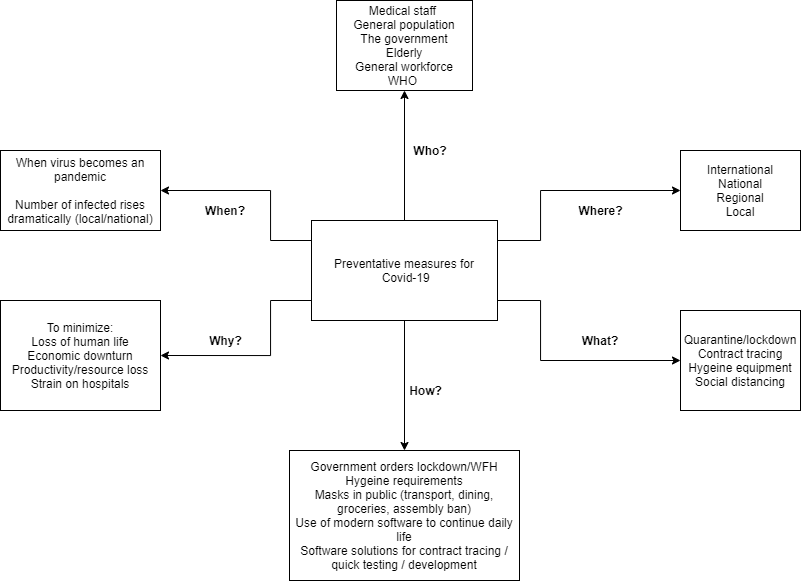
\includegraphics[width=0.75\textwidth]{0_billeder/HV-Mindmap.png}
    \caption{Mindmap of questions or, in Danish, HV-mindmap.}
    \label{fig:HV-mindmap}
\end{figure}

It was decided to continue with the questions raised regarding "how" and "why", as these branches on the mindmap aid the focus on simulation that is imperative to the project.

Our goal is to make a simulation of COVID-19 spread as well as the effects of preventive measures, namely contact tracing. Throughout our theoretical outlining, we wish to focus on software solutions that predict the spread (and how one might limit the spread) of COVID-19. Specifically, our goal is to centre our work around contact tracing as a variable as well as researching other meaningful variables that can prevent further spread of COVID-19.

Before formulating a concise problem statement, some theoretical foundation about COVID-19 is naturally needed. Therefore, the following describes several key aspects of COVID-19, such as the basic virology of the illness, SARS-CoV-2, societal factors that can influence the spread as well as several preventive measures - including contact tracing - of COVID-19.
\section{Virology of SARS-CoV-2} \label{sub:virology}

We include the virology of the specific pathogen, SARS-CoV-2, to further specify the spread of the illness in our simulation. The goal with including virology of SARS-CoV-2 is to more accurately map how the illness might spread through a population. For instance, is the illness more likely to spread among some demographics than others? Likewise, might mortality rates be higher among certain demographics than others? Lastly, do these measures warrant a specification of said demographics within the simulation? 

The virology of SARS-CoV-2 is not a field where any conclusions can be seen as being final, as it continuously gets updated when new discoveries are made. Therefore, any and all statements made in this paper regarding virology of SARS-CoV-2 should be considered arguable at best.

Severe acute respiratory syndrome coronavirus 2, also known as SARS-CoV-2 causes  Corona Virus Disease 2019 (COVID-19). SARS-CoV-2 is a highly pathogenic and very easily transmitted virus that has proven a severe threat to the health of several demographics across the world.  

The incubation period (the time from exposure to symptom onset) is set to be about 10 - 14 days, though the more standardised incubation period is set to be 14 days. If the infected person has pre-existing conditions that make them immunocompromised, the incubation period can be as long as 20 days. Similarly to incubation periods, levels of contagion can vary greatly betweeen individuals \citep{ries_how_2020}. Incubation and contagion can also be affected by the severity of the illness - ie., if the infected person has more severe symptoms, they can be considered more highly infectious.

The effect that various variables such as age, sex, pregnancy and the like have on the individual's experience with SARS-CoV-2 are disputable and as of the writing of this paper, there are few sources to draw from. However, a few conclusions can be drawn with some certainty.

Firstly, regarding sex, males are more likely to have worse symptoms and significantly more likely to die from the illness (70.3 percent male deaths versus 29.7 percent female deaths) \citep{jin_gender_2020}. This conclusion was also drawn by Kragholm et al, who further concluded that \say{men were significantly associated with higher risks of a 30-day composite endpoint of all-cause death, severe COVID-19 diagnosis, or ICU admission as well as individual components of all-cause death and ICU admission.} \citep{kragholm_association_nodate} Kragholm et al's study was conducted specifically within Denmark, making their numbers especially relevant to this project.

Secondly, regarding age, older demographics are more likely to die from the illness, especially with comorbidities \citep{jin_gender_2020}. However, younger demographics are more likely to spread the illness \citep{ssi_statens_nodate} and less likely to have severe symptoms. Asymptomatic carriers are also especially found amongst the younger demographics.

Lastly, concerns have been raised regarding pregnancy and SARS-CoV-2. WHO have found that pregnant women of all ages are more likely to be showing symptoms than non-pregnant women. WHO also note a trend for infected, pregnant women to give birth prematurely. A relatively large number (1 in 4) of babies born to women, who tested positive for COVID-19, also needed to be admitted to neonatal units. Deaths for both women and babies remain low, however \citep{who_new_nodate}. 

In conclusion, biological sex and age are virological factors that we deem more relevant to take into consideration when simulating the spread of COVID-19 than pregnancy. In a similar vein, the statistics behind the difference of severity and mortality for age and sex are more readily available. Therefore, we will divide our population in our simulation up according to sex and age as realistically as possible.
\section{Societal Impact of COVID-19}

So far, COVID-19 has had an enormous impact on societies both local and global. There has been a harsh decline in the number of people visiting the hospital, even in urgent situations. For instance, a study regarding paediatric urgency care in Italy showed a decline in visits of 84 percent from 2019 to 2020. This therefore has a long-term negative impact on paediatric health \citep{manzoni_impact_nodate}.

\begin{figure}[H]
    \centering
    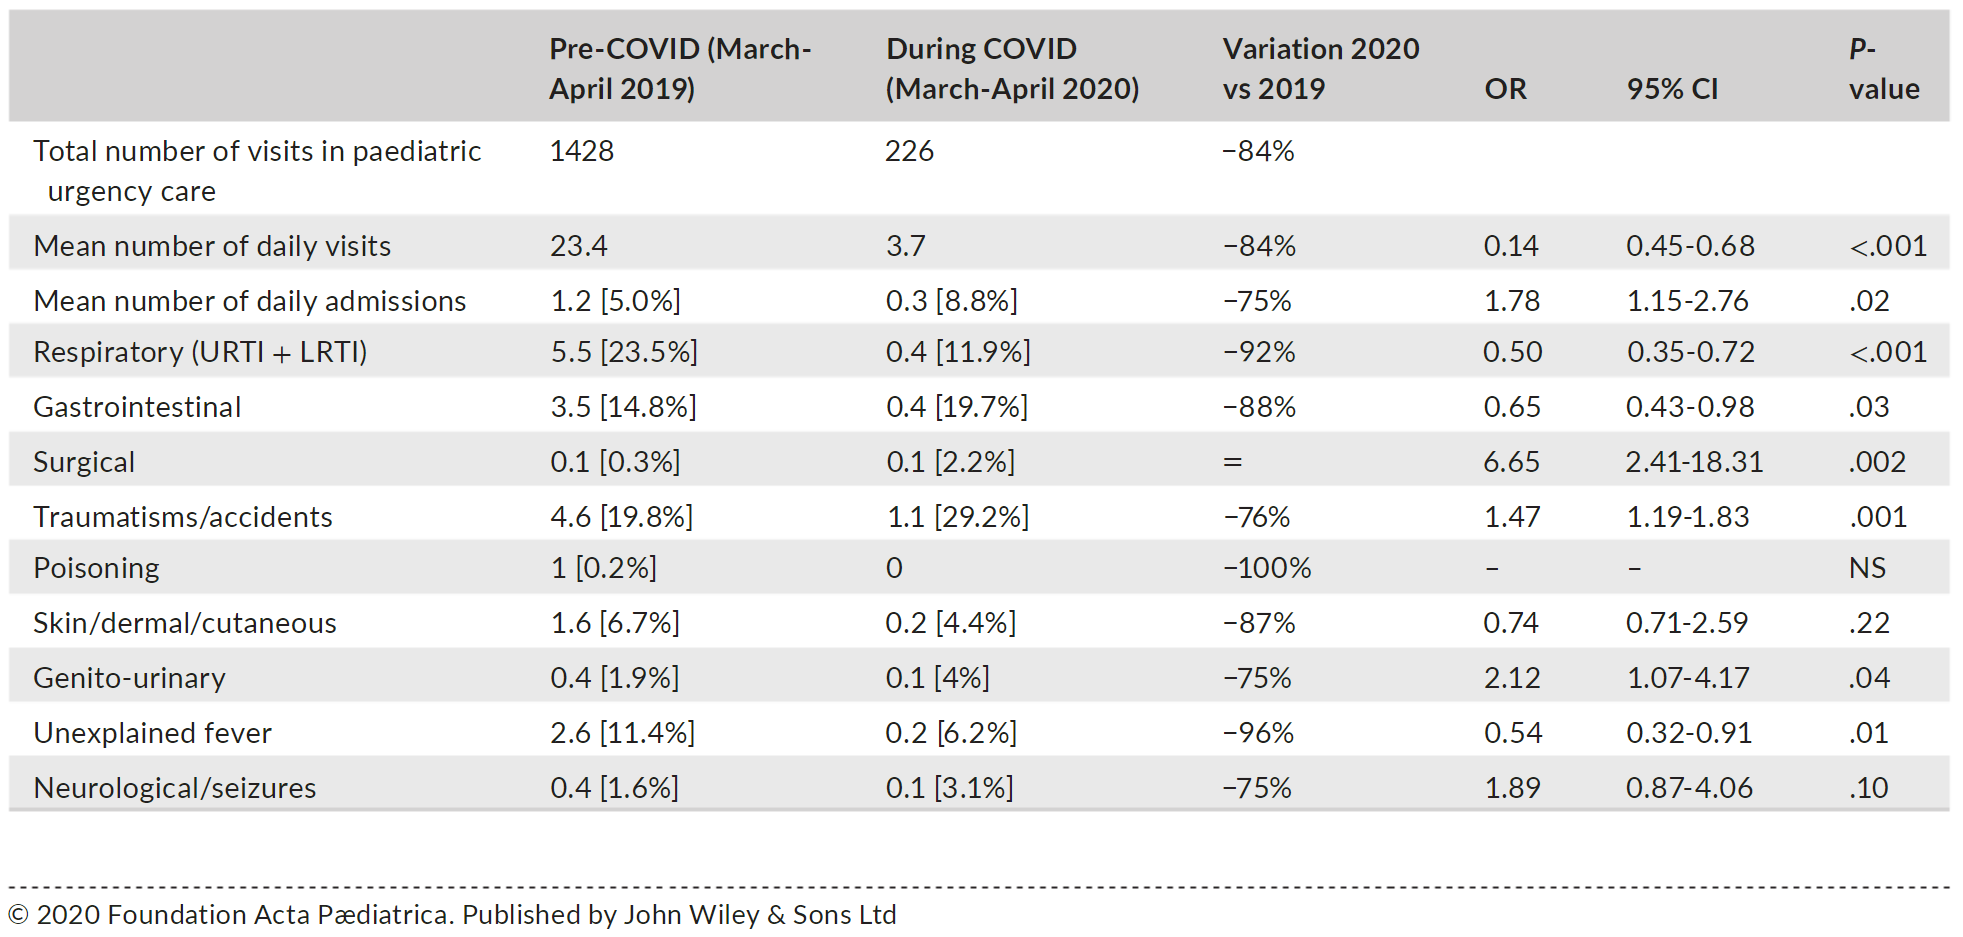
\includegraphics[width=\textwidth]{0_billeder/Covid impact hospitals.PNG}
    \caption{This table shows the visits to paediatric urgency care in 2019 compared to during COVID-19 \citep{manzoni_impact_nodate}}
    \label{fig:Covid-Hospital}
\end{figure}

Similarly, the COVID-19 pandemic has caused a tremendous surge in volatility in the stock market. Volatility is the liability of the stock market to change rapidly. This is the third highest peak since 1900, as seen in figure \ref{fig:Covid-Economy} only outdone by the great crash of Wall Street in 1929 and Black Monday in 1987 \citep{baker_unprecedented_2020}.

\begin{figure}[H]
    \centering
    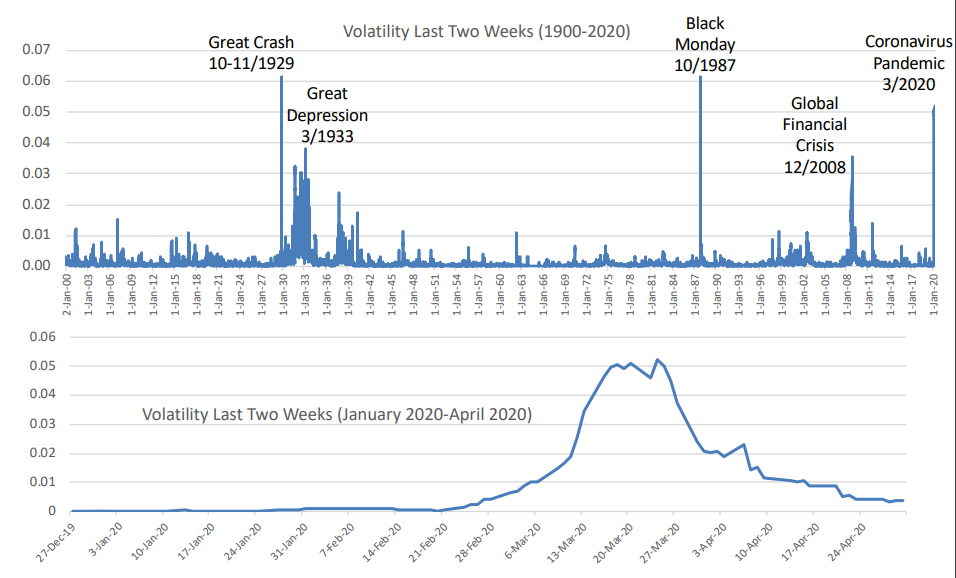
\includegraphics[width=\textwidth]{0_billeder/Covid impact Economy.PNG}
    \caption{This graph shows the spikes of volatility in the stock-market since 1900 \citep{baker_unprecedented_2020}}
    \label{fig:Covid-Economy}
\end{figure}

When dealing with a pandemic like COVID-19, it is important to consider not only the effect on mental health that may be caused by the existence of the virus alone but also the effect that preventative measures can have on mental health.

COVID-19 spreads rapidly with human-to-human contact, which in turn has caused a surge in anxiety, stress, xenophobia and the like. The consequences of these increases in mental strain on the general population has also led to behaviours like hoarding, mistrust in authority and similar that negatively affect the prevention and mitigation of COVID-19 \citep{javed_coronavirus_2020}.
\section{Societal Factors}

Different societal factors plays an important role when looking at the demographics of a pandemic. These factors are seen and described as important variables which directly affects the spreading of a virus. Generally speaking there are countless factors to consider, but these factors can all be categorised to give an overview of how big an impact these societal factors have on the spread of COVID-19. 

In regards to the spreading of COVID-19 and other pandemics, these factors can be summarised into the following:

\begin{itemize}
    \item Population density 
    \item Living conditions of an area
    \item Socioeconomic status 
    \item Sanitary facilities 
    \item Cultural aspect
\end{itemize}

Although we recognise the validity of the aforementioned factors, we will primarily argument that the population density is one of the more important factors. \citep{who_listings_nodate} In addition to the population density, the culture of a designated country or area is also to be considered, since the spreading of a virus is highly dependant on how we interact with each other - as an example, these cultural factors include greetings, social gatherings, how we socialise with family and colleagues for examples - countries with seemingly common demographics can vary in total COVID-19 infections depending on the culture of the society.\citep{fanelli_analysis_2020}

\subsubsection{Population Density}
Population density is an important factor to consider when estimating the spread of a virus, such as COVID-19. This is both in terms of the total number of contacts a person has as well as the total duration of the disease. \\
The population density has an effect that is proportional to the contact rate \citep{rocklov_high_2020} in terms of the total number of contacts. This means that it would take less time for the disease to spread in a densely populated area. This in turn ties into the population density's effect on the spread and decay duration.
\begin{figure}[H]
    \centering
    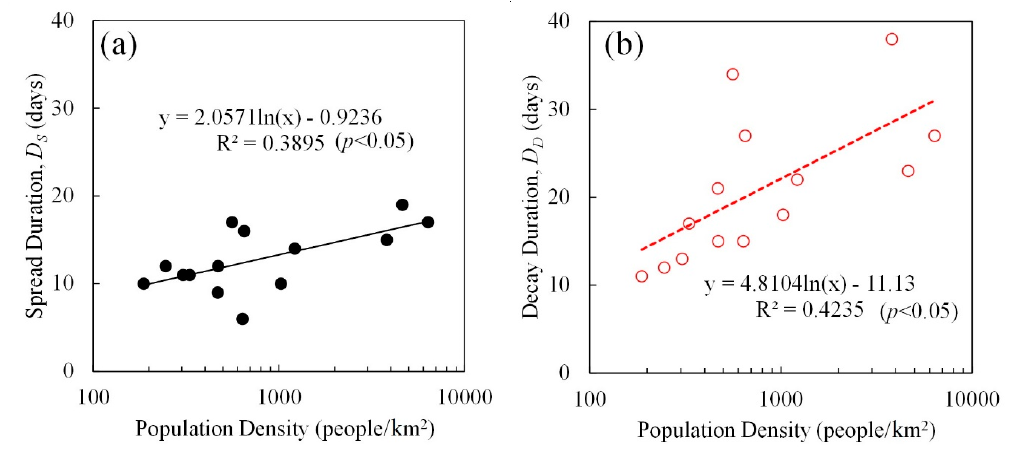
\includegraphics[width=0.8\textwidth]{0_billeder/Spread-Decay.png}
    \caption{``Relationship of the (\textbf{a}) spread and (\textbf{b}) decay duration ($D_S$ and $D_D$) with population density.'' \citep{rashed_influence_2020}}
    \label{fig:Spread-Decay}
\end{figure}
In this study, different districts in Japan with different population densities were chosen and studied, in figure \ref{fig:Spread-Decay}. The data from these districts have been plotted. There is an observable trend in this figure, which shows that population density also has a considerable effect on the spread and decay duration of COVID-19 outbreaks. 

\subsubsection{Culture}
Since it has been established that one of the main dangers of COVID-19 is how many people are gathered in a given location, cultural differences between peoples must be considered a parameter that - if nothing else - needs mentioning.

In this report, we will use the term "culture" as an umbrella term that encompasses both special occasions (Chinese New Year, American Thanksgiving etc.) and the more general way that people intermingle in their society. It should here be mentioned that scholars like Yoosefi Lebni et al. have pointed out that the cultural aspect also includes the will full endangerment of others by some people to ensure their own survival \citep{yoosefi_lebni_how_2020}. In the context of COVID-19, this cultural aspect relates specifically to hoarding and looting to ensure food and water for oneself and one's family.

Bruns et al. have pointed out that COVID-19 also greatly influenced different aspects of culture, such as greetings, major holidays and events, and interactions between family members and friendship groups \citep{bruns_covid-19_2020}. Because culture is such a vague entity, it is hard to quantify within the context of a simulation.
\section{Preventive Measures} \label{sec: preventive measure}

It is impossible to debate the spread of COVID-19 without including the numerous and different preventive measures that have been implemented both internationally and nationally. As COVID-19 can be a potentially catastrophic, global event if no global preventive or mitigative measures are implemented, it is also relevant to outline several types of preventive measures. Some preventive measures can be implemented by an individual or a group of individuals. Others are implemented by an authority like a government.

We aim to use our model to compare and contrast different preventive and mitigative measures when simulating COVID-19. Therefore, a comprehensive outlining of the many preventive measures that have been implemented within Denmark is needed. In this section, we will outline many different factors that aid prevention of COVID-19, with the goal of implementing variables with adjustable parameters into the simulation, which are relevant and plausible. While all the mentioned preventive measures might not be used for the final simulation, this will make it possible to argument, as to why we might leave some of these measures out.

\subsection{The Insecurity of Social Responsibility}

At the core of any preventive measure that spans around an entire society, whether local, regional or even global, is of course individual, social responsibility. In short, it is always up to the individual to adhere to the rules put in place by the relevant authorities, and if no rules are being forced, some form of social responsibility is still expected. A comprehensive overview of mitigative measures that can be implemented by the individual is found in \textit{COVID-19 (SARS-CoV-2) pandemic: fears, facts and preventive measures} \citep{ayenigbara_covid-19_2020}, who have also created figure \ref{fig:Mitigative-Measures}. These mitigative measures all stem from the basic principle of the individual’s own will to comply with them. Therefore, many of the preventive and mitigative measures mentioned in this report will be based - at least in part - on this figure.

\begin{figure}[H]
    \centering
    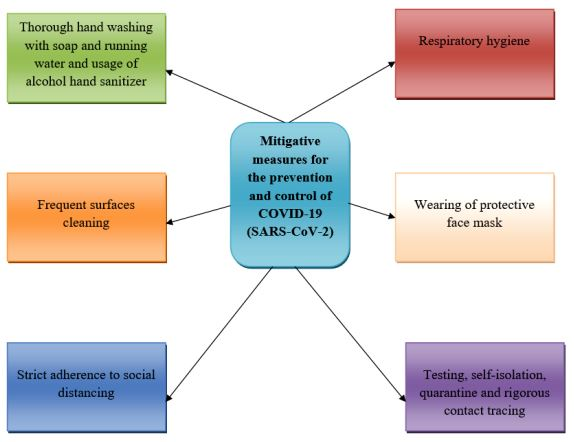
\includegraphics[width=0.75\textwidth]{0_billeder/mitigation of COVID-19.JPG}
    \caption{Mitigative measures that should be implemented across a society to combat COVID-19 \citep{ayenigbara_covid-19_2020}}
    \label{fig:Mitigative-Measures}
\end{figure}

Here, a note of definitions must be made. The word "mitigative" does of course not have the same definition as the word "preventive". Mitigative actions are not, per se, actions that can completely prevent the transmission of COVID-19, but rather to minimize the risk of rampant the spread. When discussing an illness like COVID-19, a realistic and critical view of the situation is important, and unfortunately, it is more realistic to focus on both mitigative and preventive measures, than purely on preventive measures.

As social responsibility relies heavily on every single individual in a given, geographical location, this parameter must be considered relatively insecure in nature. Therefore, social responsibility as a factor has been parted into the following multiple parameters to ensure minimal insecurity for each factor, and to ensure a way to quantify these factors. 

\subsection{Hygiene}
As shown in figure \ref{fig:Mitigative-Measures}, hygienic prevention is key for the individual to prevent spread of COVID-19 and ensure the safety of both themselves and others. Four of the six mentioned mitigative measures relates to personal hygiene or cleanliness of the environment (hand-washing, respiratory hygiene, mask-wearing, and surface-cleaning). For this report, we will consider respiratory hygiene measures as an umbrella term underneath, in which mask-wearing is the main component.

\subsubsection{Mask-wearing}
A popular means of prevention against COVID-19 amongst civilians and medical personnel alike, has been the usage of face masks- and shields. Ayenigbara et al. defines a protective face mask as a mask made of ``protective materials used to cover the nose and mouth in order to prevent the spread of highly infectious respiratory deseases like influenza, MERS and COVID-19.''\citep{ayenigbara_covid-19_2020}. Wearing protective face masks are particularly helpful in minimizing the risk of transmission via droplets, one of two main methods by which the virus spreads (The other being via touching surfaces).

Wearing masks is particularly useful in minimizing the spread, from persons who have tested positive to other persons \citep{ayenigbara_covid-19_2020}. It should be noted that wearing a mask whilst uninfected, will also still reduce the risk of transmission, though it seems rather impossible to quantity this. In short, wearing a mask both mitigates the general spread and the individual's risk of infection.

\textbf{Other Respiratory Hygiene Measures}
Other than mask-wearing, other respiratory hygiene measures can also mitigate spread of COVID-19. One such example of respiratory hygiene is sneezing and coughing into something that can preferably be immediately disposed of, such as tissue paper. 

Generally speaking, minimizing the transmission of droplets or aerosols via sneezing and coughing, helps mitigate the spread of COVID-19. The status of the virus cannot be seen as being airborne, though it cannot be ruled out, that it can spread via aerosols, as an example in ambient air. Therefore it is also of great importance to have efficient ventilation in the room you are present in. For this report we won't consider COVID-19 as being airborne, as it mainly spreads via droplets, and presumably in rare cases it can spread via aerosols in ambient air, if the ventilation is poor.


\subsection{Hand Sanitiser and Other Hygienic Measures}
While COVID-19 mainly spreads through droplets, it can also be transmitted via physical touching of surfaces or substances (and persons) that have been exposed to COVID-19. The risk of infection is highest if the eyes, nose and/or mouth is in contact with a surface, substance or person that is in contact or has been in contact with the virulent pathogen known as Sars-Cov-2 \citep{ayenigbara_covid-19_2020}. As explained in subsection \ref{sub:virology} - Virology of Sars-Cov-2, Sars-Cov-2 is the pathogen that leads to the illness known as COVID-19 or, in layman's terms, coronavirus.

Since Sars-Cov-2 is a highly contagious pathogen, it is important to maintain a high level of personal hygiene as well as hygiene in one's surroundings to minimize the risk of transmitting COVID-19. One obvious instance is through the rigorous usage of hand sanitizer and frequent hand-washing. To be at all effective, a hand sanitizer must be alcohol-based and properly and safely stored \citep{gharpure_knowledge_2020}.

While washing hands is a more thorough (if done correctly) way of preventing transmission of COVID-19, it can also be quite harsh on the skin to frequently use soap and similar cleaners - not to mention improbable in larger, semi-public areas such as supermarkets, schools and corporate workspaces according to \cite{cavanagh_rational_2020}. Therefore, hand sanitizer is the default "on-the-go" method for cleaning hands and thereby minimizing transmission through touching of surfaces. Lastly, each person should aim to touch their face as little as possible throughout their day. This measure will also aid in minimizing risk of infection via one's own mask.

\subsection{Social Distancing and Quarantine}
A parametre that is almost completely up to each individual is social distancing. Social distancing is very simply put the act of keeping a physical distance to other people whilst in public and semi-public scenarios \citep{ayenigbara_covid-19_2020}. Social distancing should be corrected to physical distancing, as social distancing would mean to take distance from all social interactions, and not just try to limit the physical interaction with other people. This would in theory mean to refrain from even meeting and socializing online, which does not make sense in form of stopping or slowing down the transmission rate of COVID-19. Physical distancing in layman's terms is better known as social distancing, so we will be using that term for the remainder of this report. Social distancing can be differentiated from quarantine and lock down, by distinguishing social distancing as preventive on a smaller scale; each person must make an effort to distance themselves from each other. Inversely, quarantine is the act of self-isolating either individually or as a household.

Measures can be taken to ensure minimal distance between two persons who, for instance, need to be closer than 2 metres to interact in relation to the exchange of goods and services. The usage of see-through plastic barriers between cashiers and customers in retail shops is one such example, where minimal distance is ensured without interfering with the experience. However, for most instances, social distancing should be considered the primary, preventive measure.

\textbf{Quarantine or Self-Isolation}

Quarantine is not a preventive measure if we assume what is to be prevented is illness. However, when it comes to a pandemic, society as a whole must aim to prevent further spread of the illness in question. Quarantine is a state of living that a person enters once they have been infected with the illness, or suspects they've become infected - in this case COVID-19. Quarantine can hereby become a preventive measure on a larger scale; when sectioning off persons infected with COVID-19, you prevent further transmission to others. During the international COVID-19 crisis, the word "self-isolation" has also been used to explain this state of living. In this report and context, the two terms are considered synonymous, regardless of etymological differences and historical applications.

As opposed to social distance, once a person has entered quarantine, they are not to interact with anyone – including within their own household. If the layout of the home permits it, they should stay completely separate from the rest of the people living with them, and cleaning should be a higher priority to ensure minimal risk of spreading via surfaces (furniture and the like) \citep{ayenigbara_covid-19_2020}. Regardless of whether a person is self-isolating by themselves or their family, the point is to mitigate contact with other people.

\subsection{Assembly Ban and Lockdown}

Although both assembly bans and lock downs can be considered part of social distance, there are some defining, differing factors. Firstly, an assembly ban or lock down is simply the governmentally implemented ban on assemblies (meaning social groups) that exceed a certain number. For instance, in March 2020, assemblies exceeding 100 people were banned by the government in Denmark \citep{ronnstad_tidslinje_2020}. This came hand in hand with the first national lock down of Denmark, in the early stages of the transmission of COVID-19 in northern Europe. 

\textbf{Assembly Ban}

Banning larger gatherings and social assemblies does not target specific social groups, religious groups or political groups when it is done as a preventive measure against pandemics. As such, while assembly bans can normally be quite polarising and controversial, they have been largely accepted by the general public across the world \citep{gostin_governmental_2020}. 

Assembly bans can, as mentioned, be given a quantifier in the form of an upper limit of individuals in a given group. This quantifier is chosen by the relevant authorities, which are Statens Serum Institut\citep{ssi_statens_nodate}, the Danish Government and the Danish Health Authority in Denmark's case. 

In March 2020, an assembly ban was introduced to Denmark. In the following five months, the assembly ban fluctuated between a maximum of 1,000 people to a maximum of just 10 people. As of the 23rd of October 2020, following a second wave of COVID-19 infections in the country, Denmark has a temporary assembly ban of 10 people or more \citep{ronnstad_tidslinje_2020}.

\textbf{Nationwide Lockdown}

Several nations have found it necessary to implement nationwide lock downs to combat the spread of COVID-19. China, Italy and the state of New York in the United States of America have all used some kind of lock down to mitigate the virus spreading. The effects of these lock downs can be seen in figure \ref{fig:Confirmed-infections-international} of confirmed infections \citep{zhang_identifying_2020}.

\begin{figure}[H]
    \centering
    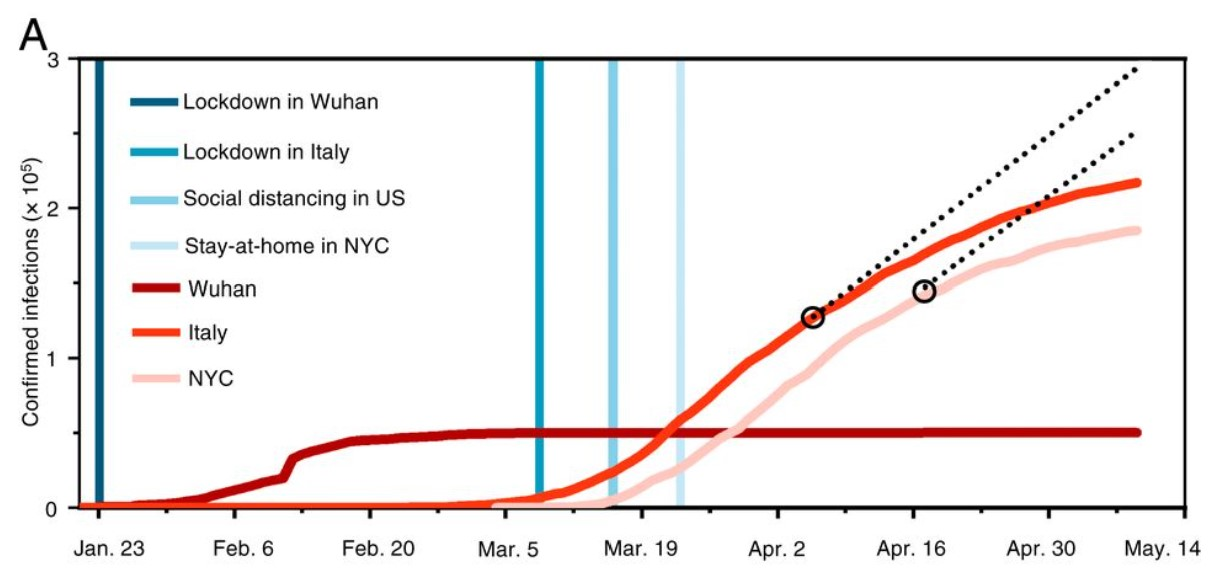
\includegraphics[width=\textwidth]{0_billeder/confirmed-infections-international.jpg}   
    \caption{Comparison of infection trends between Wuhan province, New York State and Italy including when lock down and similar preventive measures were implemented.
    \citep{zhang_identifying_2020}}
    \label{fig:Confirmed-infections-international}
\end{figure}

As shown in figure \ref{fig:Confirmed-infections-international}, the steady increase in confirmed infections was curbed after implementing either a temporary lock down, stay-at-home orders or social distancing. Lock downs can be considered the most serious implementation of what is, at its core, a form of social distancing. 

When a lock down is implemented, schools and non-essential businesses are typically closed and assembly bans are implemented. Depending on severity of the infection rate, stay-at-home orders and curfews can also be implemented. Lastly, quarantines for inbound travelers or actual bans on inbound travelling can also be implemented as part of nationwide lock down \citep{gostin_governmental_2020}.

\subsection{Information and Misinformation}

General information given to both the general public and lesser authorities within a society regarding COVID-19 is one of the most effective ways to minimize further spread of the illness. Although misinformation is of course not a preventive measure, it is a large enough factor within prevention of COVID-19 to warrant a few words on the topic. In the modern day, a lot of information can be given to the general public digitally, such as through apps and websites. This will be further outlined in subchapter \ref{Contact Tracing}.

Bierwiaczonek, Kunst and Pich have already concluded that conspiracy theories surrounding COVID-19 reduces social distancing \citep{bierwiaczonek_belief_nodate}, and Tasnim et.al have similarly concluded that the general spread of misinformation hinder the mitigation of COVID-19 on both a local and global scale \citep{tasnim_impact_2020}. Lastly, Pennycook et.al. have paid special attention to how this misinformation especially spreads on social media (Facebook, Reddit, YouTube and the like) \citep{pennycook_fighting_2020}. It can therefore confidently be stated that misinformation can be detrimental to the general prevention of COVID-19 and similar, respiratory infections.

\textbf{Trust in Authority}

The World Health Organisation (WHO) is a major authority on COVID-19 and similar health topics that span the globe \citep{who_home_nodate}. WHO collects data about transmission, recovery rates, morbidity, and the like. They also inform the general, international public about precautionary measures each individual can make use of to minimize risk of infection for both themselves and their family. 

For Denmark specifically, Statens Serum Institut (SSI) is another authority. SSI is an institute that operates under the Danish Ministry of Health. SSI is one of the main sources this paper have used to collect raw data from, such as transmission and day-by-day development of the virus’ spread within the country \citep{ssi_statens_nodate}.

\section{Contact Tracing}\label{Contact Tracing}

Contact tracing is the simple act of tracking the spread of an illness through a given population. Contact tracing is typically only used in scenarios where the illness has turned into an epidemic or pandemic - such as the case with COVID-19. In its most basic form, contact tracing can be done through word-of-mouth. In the modern world, contact tracing is typically handled by an authority with medical expertise. With new technology, contact tracing can be optimized even further.

With COVID-19 being easily spread from one person to another, it is important to identify who a person (who have tested positive) have been in contact with, within the time period that they could have spread the virus to other people. These people are called contacts, and will be observed for two weeks, to see if they develop any symptoms, and if so, if they have contracted the virus. The goal of course is to minimise the spread of COVID-19 pandemic\citep{who_headquarters_coronavirus_2020}.

The World Health Organisation have written about the several steps of contact tracing. First of all, contacts need to be defined. In short, who is considered a contact? In the case of COVID-19, the definition of a contact is ``a person who has been exposed to someone else infected with the virus that causes COVID-19, from 2 days before to 14 days after the person started to show symptoms.'' \citep{who_headquarters_coronavirus_2020}

Secondly, the defined contacts need to be identified. Here, the infected person will be interviewed,
to find out who they have had contact with \citep{who_headquarters_coronavirus_2020}. Typically, there is a special focus on contacts in the 48 hours leading up to the testing.

Thirdly, the identified contacts should be contacted to inform them. This can be done either through an app, over the phone or via e-mail to let them know that they have been contact traced and what the purpose of contact tracing is. In this context, they must also be told how their personal data is used and what it is being used for. The contact will also be informed on the symptoms to be aware of as well as how, when and where to quarantine \citep{who_headquarters_coronavirus_2020}.

Fourthly, the contact will be encouraged to stay in isolation to prevent further spreading of the disease. During quarantine, the contact should be monitored for 14 days after exposure, to see if the person develops any symptoms or gets ill. If the contact receives a positive test, they will likewise need to trace their own contacts. Lastly, the information of each contact person is stored in a database daily, updating the person's health status \citep{who_headquarters_coronavirus_2020}.

WHO adds that contact tracing does not necessarily need technological tools. The aid of digital contact tracing has optimised the process. Via digital contact tracing through usage of apps and Bluetooth, it can certainly help streamline the process of contact tracing. COVID-19 was not the first illness that modern, digital contact tracing was used for. Many solutions used for COVID-19 were originally developed to combat the spread of Ebola virus \citep{who_headquarters_coronavirus_2020}.

\subsection{Contact Tracing in Denmark} \label{Contact Tracing in Denmark}

In Denmark, citizens have the option to use the newly developed app smitte|stop for contact tracing. The app was specifically developed for contact tracing of COVID-19. With this type of digital contact tracing, a significant advantage is given each person in regards to efficiency. The app simply notifies the user if they have been in close contact with someone who has tested positive \citep{smittestop_smittestop-app_nodate}. Since a majority of people who test positive for COVID-19 are asymptomatic, this type of contact tracing can arguably minimise spread of COVID-19.

The smitte|stop app works relatively simply. It generates a random ID between users' mobile devices if two or more users have been in close proximity for more than 15 minutes in any given location. The exchange of these randomly generated IDs is done via Bluetooth. The reasoning behind the random generation is to keep each user's information separate from the app. In essence, the only information the app has access to is the device's location as well as the device's Bluetooth connection. To add further security and anonymity to the users of smitte|stop, the randomly generated IDs are updated every 15 minutes. The app itself regularly compares the collected IDs to that of the infected person. If there is a match, the app will notify you and advise you on future actions \citep{smittestopdk_download_nodate}.

Similarly, if you are the person who has tested positive, you can simply add to your app that you are now infected. The app will verify your identity through your NemID (the common, secure login solution in Denmark) to check whether you have a positive test to prevent fake positives. As a last step, smitte|stop asks your permission to share your previously generated IDs within the last 14 days. This enables the app to notify any and all people you have been in close contact with for more than 15 minutes in the last 14 days \citep{smittestopdk_download_nodate}.

To summarize, this type of digital contact tracing essentially automates and optimises the process for the population of Denmark through the app smitte|stop. An improved method for contact tracing (such as this is) is especially vital for the minimisation of spread of illnesses that present themselves asymptomatically. Since COVID-19 has proven to be largely asymptomatic, an app like smitte|stop or similar can arguably aid in prevention of spread.
\section{Scope of Project} \label{sec: Scope project}

The scope of the project encompasses usability of results and reasoning behind making the project in the first place. For this particular project, the reason behind it is to further the study of a topical illness, namely COVID-19. Therefore, the reason for this project's existence is simply to create an effective way of simulating the spread of the COVID-19 pandemic and what effect contact tracing has on it.

Of course, the source code was created with an explicit intent to input situationally specific variables and parameters of \textit{any} pandemic. This intent heightened the usability of the source code itself, although the results and analyses attached to it are only usable within the scope of the simulation (see section \ref{sec: Scope Simulation}).


\section{Problem Statement} \label{sec: Problem Statement}
After laying a proper, theoretical foundation, it is now possible to formulate a problem statement. As established, the finished problem statement must coincide with the project catalogue (Appendix \ref{P1Katalog}). Therefore, the centre of the problem statement must relate to contact tracing of COVID-19. Beyond this, we have wished to focus on how the spread of COVID-19 can be affected by contact tracing. This has led us to the following problem statement:

\begin{center}
    \textit{How to model and simulate the spread of COVID-19 in a given population with or without contract tracing? 
How can this simulation be used to extrapolate relevant conclusions with different parameters?}
\end{center}

The parameters mentioned are things such as the amount of susceptible, infected, recovered etc. This problem statement allows us to both collect and treat data relating to the efficiency of contact tracing. To properly quantify the effect of contact tracing, we will be making use of a "ceiling" - in effect, a maximal capacity. This max capacity will be hospital capacity for the given population. If contact tracing mitigates the spread enough to keep the rate of severely infected under the hospital capacity, we can conclude that contact tracing has enough of a positive effect on the pandemic.

\chapter{Simulation Design} \label{chap:simulation}

The chapter "Simulation" focuses on the design and execution of our simulation, herein the models created to help produce our simulation. These models and all factors surrounding them will be described in this chapter. However, to properly create and treat a simulation, a theoretical outline must first be written regarding simulations. 

Therefore, this chapter begins with basic theory regarding what a simulation is, what type of simulations might be relevant for this specific project, as well as the overall scope of the simulation. 

Afterwards, an explanation of the composition of our simulation follows. This explanation includes limitations within our simulation, and challenges posed by our source code as well as defences for the data used to output the raw data. 

\section{What is a Simulation?}
In this report on simulating COVID-19 we will use \citeauthor{choi_modeling_2013}'s academic definition of a computer simulation. They define these simulations as the following:

\say{A dictionary definition of simulation is the technique of imitating the behaviour of some situation by means of an analogous situation or apparatus to gain information more conveniently or to train personnel, while an academic definition of computer simulation is the discipline of designing a model of a system, simulating the model on a digital computer, and analyzing the execution output.} \citep{choi_modeling_2013}

Simulations make it possible for anyone to gain an overview of how specific events change and develop, typically over a period of time. These events could be related to businesses researching new methods, statistics for population growth or the spread of an illness. Therefore, a simulation is the ideal tool for predicting the spread of COVID-19. 

Simulation modeling solves real-world problems safely and efficiently. It provides an important method of analysis which is easily verified, communicated, and understood. Across industries and disciplines, simulation modeling provides valuable solutions by giving clear insights into complex systems.

Simulation enables experimentation on a valid digital representation of a system. Unlike physical modeling, such as making a scale copy of a building, simulation modeling is computer based and uses algorithms and equations. Simulation software provides a dynamic environment for the analysis of computer models while they are running, including the possibility to view them in 2D or 3D.

The uses of simulation in business are varied and it is often utilized when conducting experiments on a real system is impossible or impractical, often because of cost or time.

The ability to analyze the model as it runs sets simulation modeling apart from other methods, such as those using Excel or linear programming. By being able to inspect processes and interact with a simulation model in action, both understanding and trust are quickly built.
\section{Simulation Types}

Because simulation is quite a popular way to program, a lot of different simulation types exist. In this section, we will focus on describing continuous simulation, discrete event-based simulation and agent-based simulation. These three types of simulation are the ones that most closely fit the needs for our project the most, as will be made clear in their following descriptions. The goal for this section is to choose the ideal simulation type for our needs, as well as properly defend our final choice.

\subsection{Continuous Simulation}
A continuous simulation will continuously, "in real time", output the results that the simulation calculates. The results are more accurately the values and systems the simulation has to work with. This means that the simulation will process the algorithms and display the results simultaneously, and not in intervals like event-based simulation described later \citep{howard_what_2020}.

An example of continuous simulation could be video games. In a game, the program or simulation will continuously look for input from the player, while calculating every other aspect the game's real-time progression. This could be a day and night cycle, what other characters behaviour should be, or as simple as what music to play at a given moment \citep{howard_what_2020}.

In short, a continuous simulation outputs results continuously. However, it is difficult to output data in intervals, which is necessary for documenting daily updates in spread of illness. In a similar vein, the continuous simulation type depends on differential equations, which will not be necessary for this project. 

\subsection{Agent-based Simulation}
Agent-based simulation is a type of simulation which simulates individual agents and how these agents can have an effect on the system the agent is part of. These kinds of simulation can be used to study things like social and economic systems. An example of this kind of simulation would be to analyse floor traffic in a shop \citep{howard_what_2020}. -

Agent based simulation would focus on the individuals in the population and their effect on the system (in connection to the spread of a virus). Therefore, it is not ideal for this project, since we are interested in seeing the effect of the system itself.

\subsection{SIR-based Simulation}\label{sec: SIR-based simulation}
The SIR model is a commonly used mathematical model which can approximate the spread of a virus during a pandemic or epidemic. In the SIR model, population is assumed to be a fixed number \textit{N}, which is divided into three groups, susceptible(\textit{S}), infected(\textit{I}) and Removed/Recovered(\textit{R}), where it does not take in to account the amount of people dying. This is where the name, SIR, comes from. These groups are described by three coupled differential equations. When a person leaves one group, they are joining another one, so there can be kept track of every subject in the population \citep{smith_sir_2016}. The SIR model can be used both in discrete-event simulation and in continuous simulation. 

Again, as described above, the only difference is that the continuous simulation will send results continuously and discrete-event based will output in intervals. For the spread of a disease these intervals would most likely be once every day, week or month, depending on the time-span of the simulation \citep{ozmen_analyzing_2016}. The SIR model is the most basic model for a simulation within the epidemiological field. So the SIR model is ideal when dealing with simulating a disease like COVID-19. This also why a SIR-based simulation is the inspiration for our final mode. Unfortunately, it does not quite cover our needs, which leads us to the last simulation type, the discrete event-based simulation.


%It also helps see faults in our simulation, if there are any individuals missing at the end of the simulation, then we know there is a fault in the code.


\subsection{Discrete Event-based Simulation}
A discrete event simulation is a type of simulation that simulates the whole program continuously, but will output the results at predefined intervals. These can be at specific time stamps or only when changes happen \citep{howard_what_2020}.
\begin{figure}[H]
    \centering
    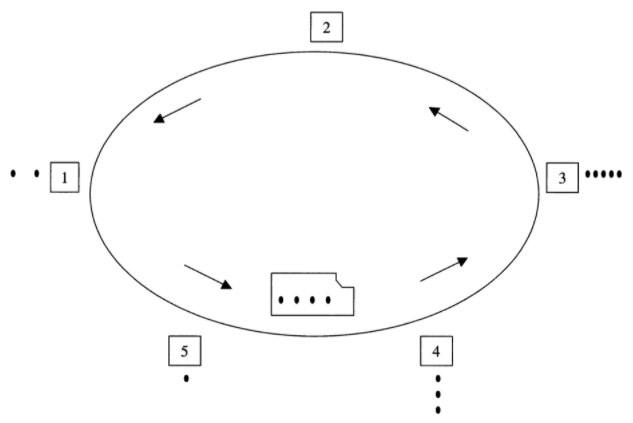
\includegraphics[width=0.75\textwidth]{0_billeder/BusModel.png}
    \caption{Bus Model \citep{fishman_discrete-event_2013}}
    \label{fig:Bus Model}
\end{figure}

Discrete event-based simulation can be looked at like a bus route in figure \ref{fig:Bus Model}. If you were to count the number of passengers on a bus, there would be no need to continuously count them when the bus is driving, as the only time the number of passengers would change is when the bus stops at a bus stop. A simulation of the same bus route would continuously calculate the amount of passengers getting off the bus and the amount of people waiting for the bus. However the simulation would only output the amount of passengers in the bus once every stop \citep{fishman_discrete-event_2013}. 

For simulating the spread of COVID-19 this simulating type is ideal, because our goal is to get a status every day, of how many have been infected, recovered etc. So in our simulation the "bus stop" is every passing day, and here the current status will be output. Therefore, while our simulation is inspired by the SIR-model, the foundation of the code is based on a discrete event-based simulation.


\section{Scope of Simulation} \label{sec: Scope Simulation}
Within the scope of our simulation, we have chosen to focus on a smaller, geographical area. We initially set the population to be the greater Aalborg area, which has a population of 217,094 people \citep{sundhedsstyrelsen_by_2020} as of 2020. Because of the fairly large population size, special attention was paid to computational efficiency (see section \ref{sec: limitations and challenges}).

Since there are limitations to simulating in C, it was decided to have a smaller population size. Therefore, the final scope of the simulation is the centre of Aalborg, which has a population of 12,366 people as of 2020 \citep{sundhedsstyrelsen_by_2020}. By having a scope with a generally homogeneous population density, the simulation itself likewise becomes quite homogeneous.
\section{Models}

This section is dedicated to the two different models that have been used to map out our simulation. Firstly, we have used the MoSCoW method of prioritisation to decide on what must, should, could and will not be in our simulation. Secondly, we have created a flowchart over the simulation to more effectively communicate the structure of the program. The goal of using these two models is to create an overview of and guideline to the program.

\subsection{MoSCoW Method}

The MoSCoW method is used to make decisions on what elements must, should, could and will not be included in a product. The elements that must be included are elements that is absolutely necessary for the product to function at all. These therefore have the highest possible priority. The further right in the diagram the less necessary the element is to the core function of the product, these however might add more details which can make the product more accurate. The elements that will not be included, might be elements taken out due to time constraints in the project. They could also be elements that are unnecessary or not in focus in our project.

\begin{center}

\begin{tabularx}{0.9\textwidth} { 
  | >{\raggedright\arraybackslash}X 
  | >{\raggedright\arraybackslash}X 
  | >{\raggedright\arraybackslash}X
  | >{\raggedright\arraybackslash}X| }

 \hline
 \multicolumn{4}{|c|}{Simulation} \\
 \hline
  Must &  Should & Could & Will not \\
 \hline
   -Contact tracing \newline -Static R-value \newline -Time frame \newline -Medical states \newline -Population 
 
 & -Incubation \newline -Hospital Cap. \newline -Demographics \newline -Severity and death
 
 & -Fluid R-value \newline -Immune response period \newline -Other preventive measures
 
 & -Mutations \newline -Culture \newline -Living conditions \newline -Climate \newline -Misinformation \\
 
\hline
\end{tabularx}

\end{center}

The choices in the must-have column reflect what has been deemed absolutely necessary to make a useful simulation. If these factors are excluded, the simulation simply wouldn't work. The factors in this column are simply put the values from the SIR-model \ref{sec: SIR-based simulation} and contact tracing, which is the focus of our project. The population is included here because there needs to be a population of people to infect so the simulation can progress. The R-value represents the average amount of people an infected person will infect in the period they are sick. It has been set as a static value here to simplify it.

The time frame is necessary since the simulation needs to run for a certain amount of time to output several, different values. The length of this time frame directly affects whether the results will give an accurate representation of reality, since a short time frame might not show when the infection dies out, which can give unusable results. 

In a similar vein, different medical states are important so a person can be determined to be susceptible to, infected by or recovered from COVID-19. Lastly, contact tracing has been deemed as a must-have because it is a requirement in the chosen project.

The different factors in the should-have column have been selected because they are important for the simulation to be more accurate, but not necessary for the simulation to function. Factors like hospital capacity, demographics and severity would create a more lifelike simulation, and therefore, they have been included in this column. Incubation has been included to delay infection chance, as is also the case with real-world data.
 
The factors in the could-have column are elements that might make the simulation even more precise and realistic, but not deemed necessary for the simulation to run well. The R-value, which has been set as static in the must-have column would most likely change as a result of several variables' influence. Therefore, a static R-value is considered a must-have, where an R-value that is interdependent on other variables is considered a could-have.

Occurrences of people getting infected twice or more with COVID-19 suggest that an individual has an immune response period after which they would be able to get infected again. As there are varying opinions on re-infection chance among scholars at the time of writing \citep{malkov_simulation_2020}, this was given a lower priority. Lastly, other preventive measures (as mentioned in subsection \ref{sec: preventive measure}) will make for a more accurate representation of contact tracing's effect on prevention, but is not necessary to gain an insight into contact tracing's effect on its own.

Lastly, the factors placed in the will-not-have column are elements that are either beyond the expertise of the group or deemed irrelevant for the simulation. For instance, mutations of the virus, while intriguing, would influence the very basis of the study, as the study is focused on COVID-19. Likewise, including misinformation (\say{fake news}) as a variable in the program arguably makes for a more precise simulation, but misinformation is not easily implemented into a program. The remaining factors in this column (culture, living conditions and climate) have been left out of the program because of time constraints and minimal relevance for the project.

After getting a better understanding of what elements are essential for our simulation through the use of MoSCoW, we were able to start designing our program through flowcharts.

\subsection{Flowcharts} \label{sub: flowcharts}
We have used flowcharts to get a more thorough understanding of how our program will work before we actually make it. The flowcharts included below are the newest version. Our first draft of a flowchart for the most basic version of our simulation can be seen in appendix \vref{Appendix:FirstFlowchart}. Below is a walk-through of the finished flowchart, which most accurately resembles the source code. The flowchart has been divided into two parts for readability.

\begin{figure}[H]
  \centering
  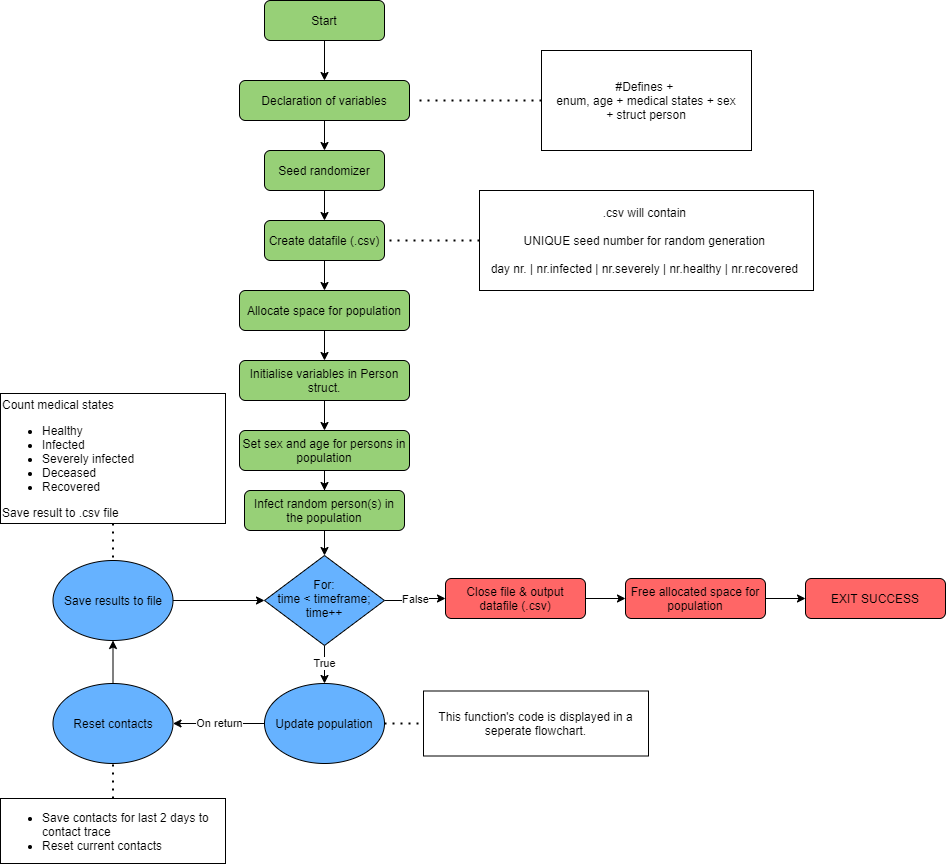
\includegraphics[width=\textwidth]{0_billeder/Part1Flowchart.png}
  \caption{Part 1 of the flowchart, the core program.}
  \label{fig:Part1Flow}
\end{figure}

In the first part seen in figure \ref{fig:Part1Flow} is the core part of our program, with the declaration/initialisation phase(marked in green), the main loop of our program(marked in blue) as well as the end of the program when the main loop is exited(marked in red).

The main loop includes functions that update the population, resets the contacts which the infected has been in contact with and saves relevant data to an output file. The update population function will be described further below in figure \vref{fig:Part2Flow}, since its the most important function. 

\begin{figure}[H]
  \centering
  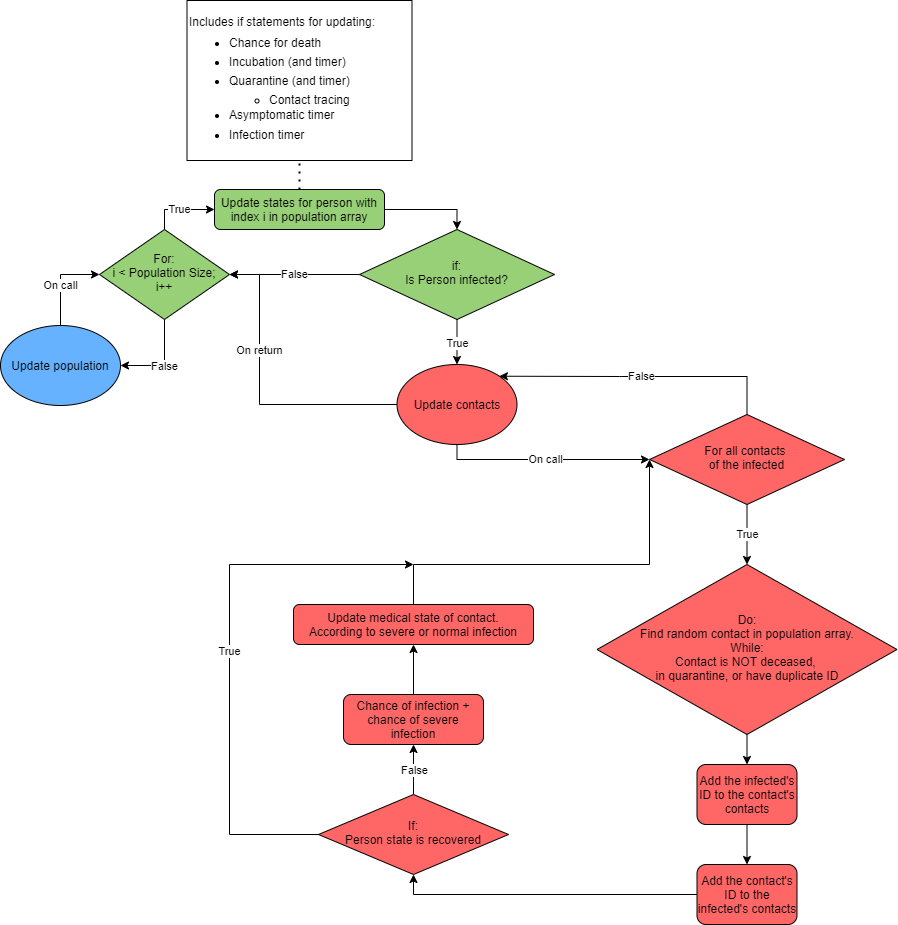
\includegraphics[width=\textwidth]{0_billeder/Part2Flowchart.png}
  \caption{Part 2 of the flowchart, extended program.}
  \label{fig:Part2Flow}
\end{figure}

As seen in figure \vref{fig:Part2Flow}, it continues from the function that updates population (in blue, leading to green). Within this function, the program runs through the entire population to not only check whether the given person is infected, but also to run through their contacts (in red). If the person is not infected, a new person is checked. However, if the person is infected, it continues to the next function call (in red).

The function that updates contacts checks through all contacts of the person. If the contact is not deceased, in quarantine or has already been checked, the contact and person exchange ID's, so they can not be re-selected as a contact until the contacts are reset. 
If the contact is susceptible, there is a chance they can become infected, after which their medical state is updated accordingly. Update contacts runs until the infected has no more contacts, after which the program loops out of the function.
\section{Our Simulation}
%VI SKAL FIXE LINJETAL FOR KODEN

Within this section, we will walk through key features of the simulation to properly explain the structure of the code. Special attention will be paid to central function calls, as it was in section \ref{sub: flowcharts}. 

In a similar vein, key aspects of the simulation will also be outlined and defended in this section. Key aspects include defence of data chosen, debugging tools and the usability and versatility of the code itself for future research.

\subsection{Key Elements in Our Simulation}
While creating our simulation, we took a lot of inspiration from one of most well-known infection simulations which is the SIR-model, that is described in section \ref{sec: SIR-based simulation}. This inspiration was primarily based in how we wanted to separate the population in terms of states. The skeleton of the code is primarily built around the discrete event-based simulation type.

We defined four medical states in our program which the population could switch between. These states are as follows: Susceptible, infected, recovered, and deceased. These were defined in a global enum, making it possible for us to easily change and check the states of the population across different functions.

\begin{lstlisting}[language=c, caption={Enum Medical States}, captionpos=b, label={snippet:EnumStates}]
enum states
{
    susceptible,
    infected,
    recovered,
    deceased
};
\end{lstlisting}

Our simulation primarily revolves around state changes in our population array, which is a struct array of the Person struct. The Person struct is defined in the beginning of the program and can be seen in its full form in snippet \vref{snippet:PersonStruct}. By changing each person's state and logging these changes accordingly, we can trace the spread of infection.

Our simulation starts with defining all the parameters that we use throughout the code, so they are together at the top and easily accessible. This makes it possible to easily configure all the parameters instead of having to change a given number. The accessibility and use of the defines are described thoroughly in section \vref{Usability and versatility of the code}.

\begin{lstlisting}[language=c, caption={Person Struct}, captionpos=b, label={snippet:PersonStruct}]
struct Person
{
    int ID;
    int age;
    int sex;
    int state;
    int asymptomaticTimer; 
    int incubationTimer;
    int infectionTimer;
    int quarantineTimer;
    int infectionPeriod;
    int numOfContacts;
    bool incubation, severelyInfected, quarantine;
    int contactID[avgContacts], tracingID[avgContacts * 2];
};
\end{lstlisting}

In the struct in snippet \ref{snippet:PersonStruct} are all the relevant variables which are used, to activate a state change (i.e. Timers and age), indicate a sub-state (i.e. incubation, etc.) or enable contact tracing (i.e. all of the IDs and the number of contacts).

The simulation runs a number of times to get an average and thereby a more accurate result. We will refer to each of these runs as a drop, as is customary within simulation. These runs happen in the main loop of the program which can be seen from line 110 - 167 in the source code in appendix \vref{Appendix: SourceCode} and it has also been described as pseudocode below. \\

\begin{algorithm}[H]
    \For{each drop}{
        Allocate memory for the population (struct array) \\
        Initialize variables of the population arrays \\
        Call a function to set age and sex of the population \\
        Start infection by infecting some of the population \\
        \For{each day}{
            \emph{UpdatePopulation:} function call to check and update the states in the population \\
            \emph{ResetContacts:} function call to store contacts for tracing and resetting contacts so new ones can be selected for the next day. \\
            \emph{SaveResults:} function call to store all of the relevant data for later output in a .csv file.
        }
        Free the allocated storage for the population array
    }
    \caption{Pseudocode for the main loops of the simulation \label{pseudo: main loop}}
\end{algorithm}
Each time the program runs through the drop for loop described above, a simulation is completed and its data is stored.

\subsubsection{UpdatePopulation function}
Our UpdatePopulation function on line 224-314 in appendix \vref{Appendix: SourceCode} goes through the whole population array and updates their medical state through various if-statements, according to their current state and timers. 

First off, we generate a random number to simulate the chance of someone dying of COVID-19. The chance of dying correlates to what age group a person is in, as is in accordance with real world data. This works through an if-statement that checks if they are severely infected and not already deceased, and if the chance hits, then they are set to deceased.

Afterwards, we have three if-statements that check if the person is infected, is in quarantine or is currently in incubation state. If so, the incubationTimer, quarantineTimer and infectionTimer for the given person ticks down. They also remove the infection state, incubation state and quarantine state if their individual timer reaches zero.

The next if-statement in UpdatePopulation runs contact tracing. It checks if a person is infected and whether their incubation period is over. If both are true, they get put in quarantine with a random amount of the 20 people they have been in contact with the last two days. The way contact tracing works is with the person struct's IDs that gets exchanged with the contacts that are generated for them if they were infected. We have an UpdateContacts function call that is described further below, where the ID exchange and more is described.
The ID's are stored for the last two days of the simulation, a random number between 5 and 20 is then generated when a person is infected and no longer asymptomatic, this then determines how many of their contacts will get traced and put into quarantine. Simulating the random amount of people one is able to remember that they have been in contact with.

Lastly in the UpdatePopulation function we have three if-statements. The first if-statement sets the asymptomatic timer to -1 if the asymptomatic timer is 0. This makes sure that they wont enter a loop, where they continuously get put into quarantine.
The next if-statement is where the UpdateContacts function is called, and it is only called for infected persons.
And the last if-statement takes asymptomaticTimer and infectionTimer down by 1, until they are healthy again.

\textbf{The UpdateContacts function} is called within the update population whenever an infected has been found, it can be seen in the code from line 317 - 370. This function finds suitable contacts for the infected (i.e. not in quarantine, deceased, etc.). After a contact is found, they exchange ID's with the infected, which ensures that the contact can not be selected again and that it can be traced. If the contact is susceptible they have a chance of being infected, if that happens their state is updated to infected and their incubation period as well as their asymptomatic period is set. Lastly they have a chance of becoming severely infected, which we define as an infection requiring hospitalisation.

\subsubsection{ResetContacts function}
The ResetContacts function is an essential function that is part of the main loop in the program. This function ensures that the contacts each person has had throughout that day is reset before the next day starts, it also stores the same contacts in the persons tracingID array, so that they can be traced if necessary. On uneven days, the first half of the tracingID array is overwritten, and on even days, the second half gets overwritten. This is because we contact trace 48 hours(2 days) back in time.

The remaining functions are mostly nonessential for the simulation part of the program, these are functions such as SaveResults, countState, etc. However, they do support the program and save the results for the simulation. Because these are not essentiel they will not be explained in further detail, but they can be seen in the source code in appendix \ref{Appendix: SourceCode}.


\subsection{Usability and Versatility of the Code} \label{Usability and versatility of the code}

As has been stated several times throughout this report, the COVID-19 pandemic has laid the foundation for many different studies - unfortunately leading to much contradictory data regarding mortality rates, risks of infections, efficiency of certain preventive measures, etc. 

The code has specifically been written with this uncertainty of data in mind. Therefore, the code uses several symbolic constants that can easily be changed (E.g. timers, periods, number of contacts) when data regarding spread and mitigation of COVID-19 becomes more certain. This increases the code's usability and versatility, making it possible to run the code with completely different parameters at a moment's notice.

For instance we have our infection period set to 10(days) where there might be published some new data, which sets it to a different number of days. In such situations, it can be easily configured to newly published data. 

Similarly, population size and the like can easily be changed, so the simulation can be applied to an entirely different, geographical location than the one used as an example in this project (Aalborg, Denmark). When more congruent data of COVID-19 has been found, this code can be updated accordingly. 

\subsubsection{Debugging Tools}

It was decided to leave in the debugging tools in the code. This was done to further support the usability of the code for further study. By leaving in debugging tools, the code can more easily be adjusted to other simulations of COVID-19 and, arguably, other pandemics/epidemics. An example of this would be our save drop function which can be seen on line 541 - 564 in appendix \ref{Appendix: SourceCode}, which can save an individual drop of a simulation in the data file. This is useful if a certain drop is giving unexpected results.

\subsection{Data used in Our Simulation}

Since the aim is to simulate a realistic depiction of spread of COVID-19, variables and parameters within the code have been decided upon based on real (or realistic) numbers. In instances where there are no (or contradictory) sources, logical estimates have been made based on similar situations. These estimates will naturally be defended whenever applied.

\subsubsection{Age/sex demographics and mortality rate}
For instance, the age groups in the code are based on demographic data from Globalis, a digital reference work funded by the UN \citep{globalisdk_danmark_2020}. The data is based on the entire population of Denmark, which has simply been laid out as a percentage distribution. This percentage distribution is one of the few instances of non-symbolic constants, since they are specific to Denmark's population. By using up-to-date data, a more realistic simulation of the spread can be achieved. As mentioned above, this is especially important due to mortality rates among elderly patients.

\begin{table}[H]
	\centering
	\begin{tabular}{ccccccc}	% Afstem antal tegn og kolonner! (l for venstre, c for center, r for højre)
		\toprule
		Age group & People hospitalized & People deceased & Cases & \% Hospitalized & \% Deceased \\\midrule
		0-59 & 2202 & 29 & 82770 & 2.66\% & 1,3\%           \\
		60-69 & 919 & 82  & 7322 & 12.55\% & 8.923\%           \\
		70-79 & 1301 & 255 & 4510 & 28.847\% & 19.6\%           \\
		80-89 & 1005 & 347 & 2135 & 47.07\%  & 34,53\%         \\
		90+ & 260 & 191 & 620 & 41.935\% & 73,5\%         \\
		\bottomrule
	\end{tabular}
	\caption{Overview over cases.}
	\label{tab:cases}
\end{table}

%The age groups are also separated by sex, but lack of proper data to correlate mortality rate to the different sexes, meant that this was omitted as factor, but it can be implemented without much trouble, since the simulation was coded with sexes as a factor in mind.

\subsubsection{Reproductive number (R-Value)}
A piece of data that was particularly hard to find was the R-value. The R-value represents a given disease's ability to spread. For instance, an R-value of 1.0 would give a completely linear \say{growth}, meaning the disease would neither increase nor decrease. When the R-value is larger than 1.0, the disease will spread. When the R-value is smaller than 1.0, the disease will die out.

While the concept of the R-value is quite straightforward, the implementation is not. An R-value is dependent on several factors, and it varies depending on country. Similarly, it can also fluctuate when the many different factors change. Therefore, while we have made use of a static R-value, a fluid R-value would have made for a more precise simulation. For this simulation we have used the estimated $R_0$ that oxford's university has come up with, which is 2.63.
\say{SARS-CoV-2, the coronavirus that has caused the covid-19 pandemic, has an estimated $R_0$ of around 2.63, says the University of Oxford’s COVID-19 Evidence Service Team. However, estimates vary between 0.4 and 4.6.} \citep{mahase_covid-19_2020}

\subsubsection{Virology data}
Most of the other numbers which we have used in the simulation are based partly on our assumptions, partly on the research we have read and partly on what we thought would work best in our simulation. This is because at the moment of this report being written there is a lot of studies and information about the virus, which have conflicting estimates of things like the infection period, incubation period, pre- / asymptomatic period. This is also one of the reasons that versatility has been considered, and these factors have been placed at the top of the code, so they easily can be updated to more accurate data.

\subsubsection{Contact tracing}

% Argue for all the numbers we use in the code here

% Deathrate pr age group

% Severity pr age group

% Avg contacts

% Quarantine period - from contact tracing

% avg infection period 

% incubation period

% traceable contacts

% contact tracing start time


\section{Limitations and Challenges} \label{sec: limitations and challenges}

There are several potential limitations and challenges that can occur in a program. For the sake of transparency, some of the limitations of our source code as well as 

\subsection{Randomisation of larger populations}

The C functions "rand" and "srand" are functions that are used to randomise within a program. These rely on the value "RAND MAX", which is 32,767. The function is not able to find a random number which is larger than this. If the simulation were to be scaled up, another method of generating random numbers would have to be found. When choosing contacts with a random value, and then checking if they will get infected with a random number, the number of people who will get checked are only the ones within the 32,767. If the simulation was scaled to anything larger than a population of 32,767 people, the program would simply stop infecting people. This is not a limit to the C language, but rather our program. Given the wide-spread usage of C, we would assume there exists a way to generate larger random number. However the group didn't have time to do further research, especially given how the actual size of the simulated population is 12500.

\subsection{Limited Population Size}

When we constructed the array with our population, we ran into a challenge where the population could not be much larger than 12,500 people. This would maybe have been fine when creating a simulation on this small of a scale. But if the simulation were to be scaled up at all, a solution had to be found.

We found our solution in the function "calloc". When initialising an array normally, the size has to be allocated statically. This can create a problem with the memory allocation, which will make it impossible to run the simulation. However, when using "calloc", the memory is allocated dynamically and then freed when the function "free" is called. This ensures the simulation cannot run into a memory error. Therefore the simulation can run with a much larger population size.

\subsection{Statistical Uncertainty} \label{sub: Statistical Uncertainty}

It has been a challenge to find some consistent values for mortality and severity since the values change from day to day. For example, SSI publishes new data each day at 2.00 PM which sometime change dramatically from the day before. This increases the uncertainty of whether or not our simulation represents a real-life situation and also if the contact tracing functions as intended.

Since COVID-19 officially started in China during December 2019 \citep{gorbalenya_severe_2020}, quickly transforming into a global pandemic, there have been differing and sometimes contradictory statements regarding data for the spread and containment of the illness. 

Included in this challenge are factors such as, which sources are up-to-date and relevant. For the data to be up-to-date for this particular project, it cannot have been published during the early days of COVID-19, which we have loosely estimated to be March 2020. Any sources from this period, while imperative to document the pandemic, are arguably uncertain, since the world knew little to nothing about the nature of the disease at that point in time.

Sources being relevant to the scope of this particular problem is naturally necessary for them to be included in this project. Since the geographical scope is limited to a region of Denmark, sources that focus on other parts of the world are only peripherally relevant to this project. However, during instances where there is no data to be found for our specific, geographical scope, we must extrapolate data from other geographical scopes. This can lead to uncertainty.

Similarly, our primary source for mortality rate is \cite{ssi_statens_nodate}, whose data is of course based on a spread that is already mitigated. Since Denmark has used preventive measures such as

\subsection{Disappearing People in Population}
Due to the natural type specifics of integers and doubles, and the way they behave with each other, we had issues regarding the amount of people in our array of structs. Often at times after we completed a run of the simulation, the data file which results are saved to, indicated that the simulation initialised a population size of ±2 to the defined population size. This was due to an incorrect mixture and deployment of the C functions "ceil" and "floor". These functions round values up and down, respectively.

In the early stages of developing the simulation, we realised it would be necessary to typecast doubles to integers. We had integers calculated and returned from functions, such as an integer of 15 people divided by 100 days, returning a 1.5 double. To use this double value, it first needs to be assigned as an double through typecasting the integer to the double type, which then allows for using the proper value for calculation of percentages.  

The final solution to the disappearing people in the population was simply to calculate using only doubles. While this does give decimal-point numbers for medical states, it keeps the population stable and, in the end, leads to more precise calculations within the simulation.

\chapter{Results and Analyses} \label{chap:result}

This chapter is dedicated not only to give an overview of the results of the simulation, but also to analyse the given results within certain parameters. This chapter is, in essence, where the problem statement in section \vref{sec: Problem Statement} can finally be answered.

The results shown and analysed are all based on the same seed (the seed being 808420), making it possible to reproduce the results both with and without contact tracing. 

We have created our results by simulating 1,000 drops with and without contact tracing enabled. In the following sections the two simulations will be compared, to each other and also to the real world. This is done by plotting the data found in Appendix \ref{Appendix:Data} onto graphs, these then visualises the differences and can be analysed. 

\section{Results from the Simulation}

To create a baseline for the remainder of the results of the simulation results, we will first outline and analyse results from the simulation, with the standard parameters for the virus and contact tracing, which we have defined and described in the previous chapter in section \ref{subsec:Data in Sim}.

\begin{figure}[H]
    \centering
    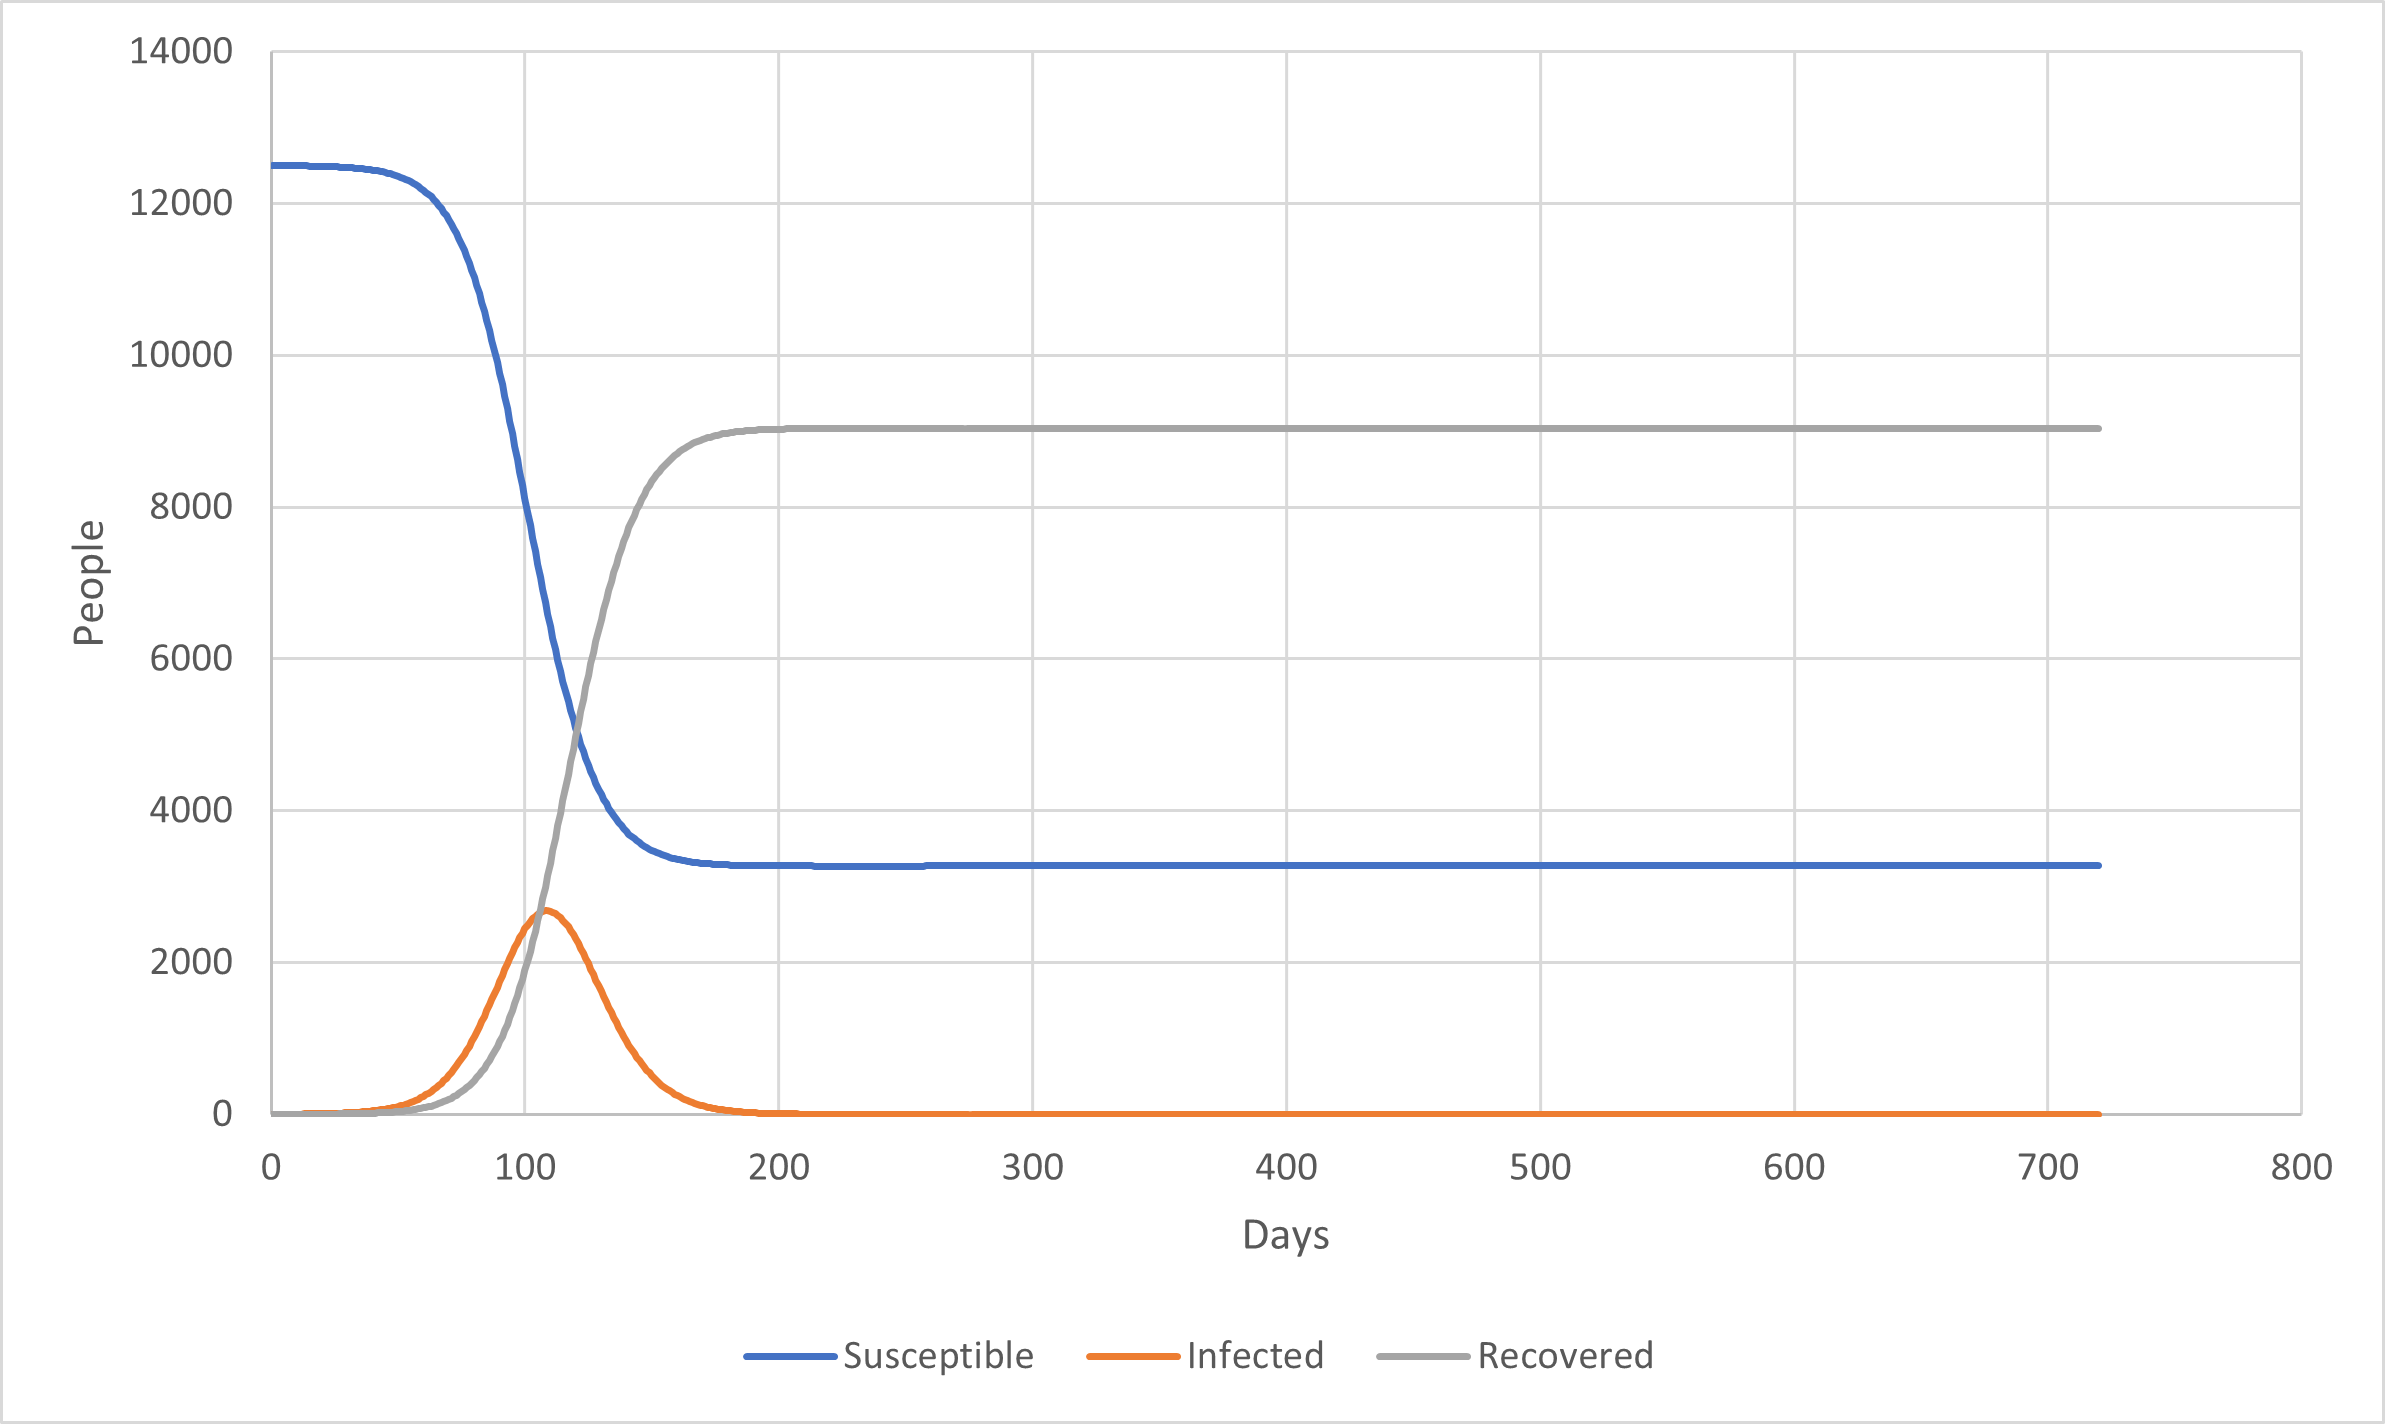
\includegraphics[width=0.75\textwidth]{0_billeder/Sim_CT_OFF.png}
    \caption{Graph of susceptible, infected and recovered plotted against days, from simulation without contact tracing}
    \label{fig:Sim_CT_OFF-1}
\end{figure}

Figure \ref{fig:Sim_CT_OFF-1} is a graph showing how individuals in the population slowly change status throughout the time frame with no contact tracing to mitigate the spread.

As is shown in \ref{fig:Sim_CT_OFF-1}, the infection peaks and dies out rather quickly (within the first 200 days). By the end of the time frame, some people remain uninfected (susceptible), while the majority of the population have recovered. It should be noted that the \say{recovered} state includes those who have survived and succumbed to the infection. This is quite different from figure \ref{fig:Sim_CT_ON-1}, as shown below.

\begin{figure}[H]
    \centering
    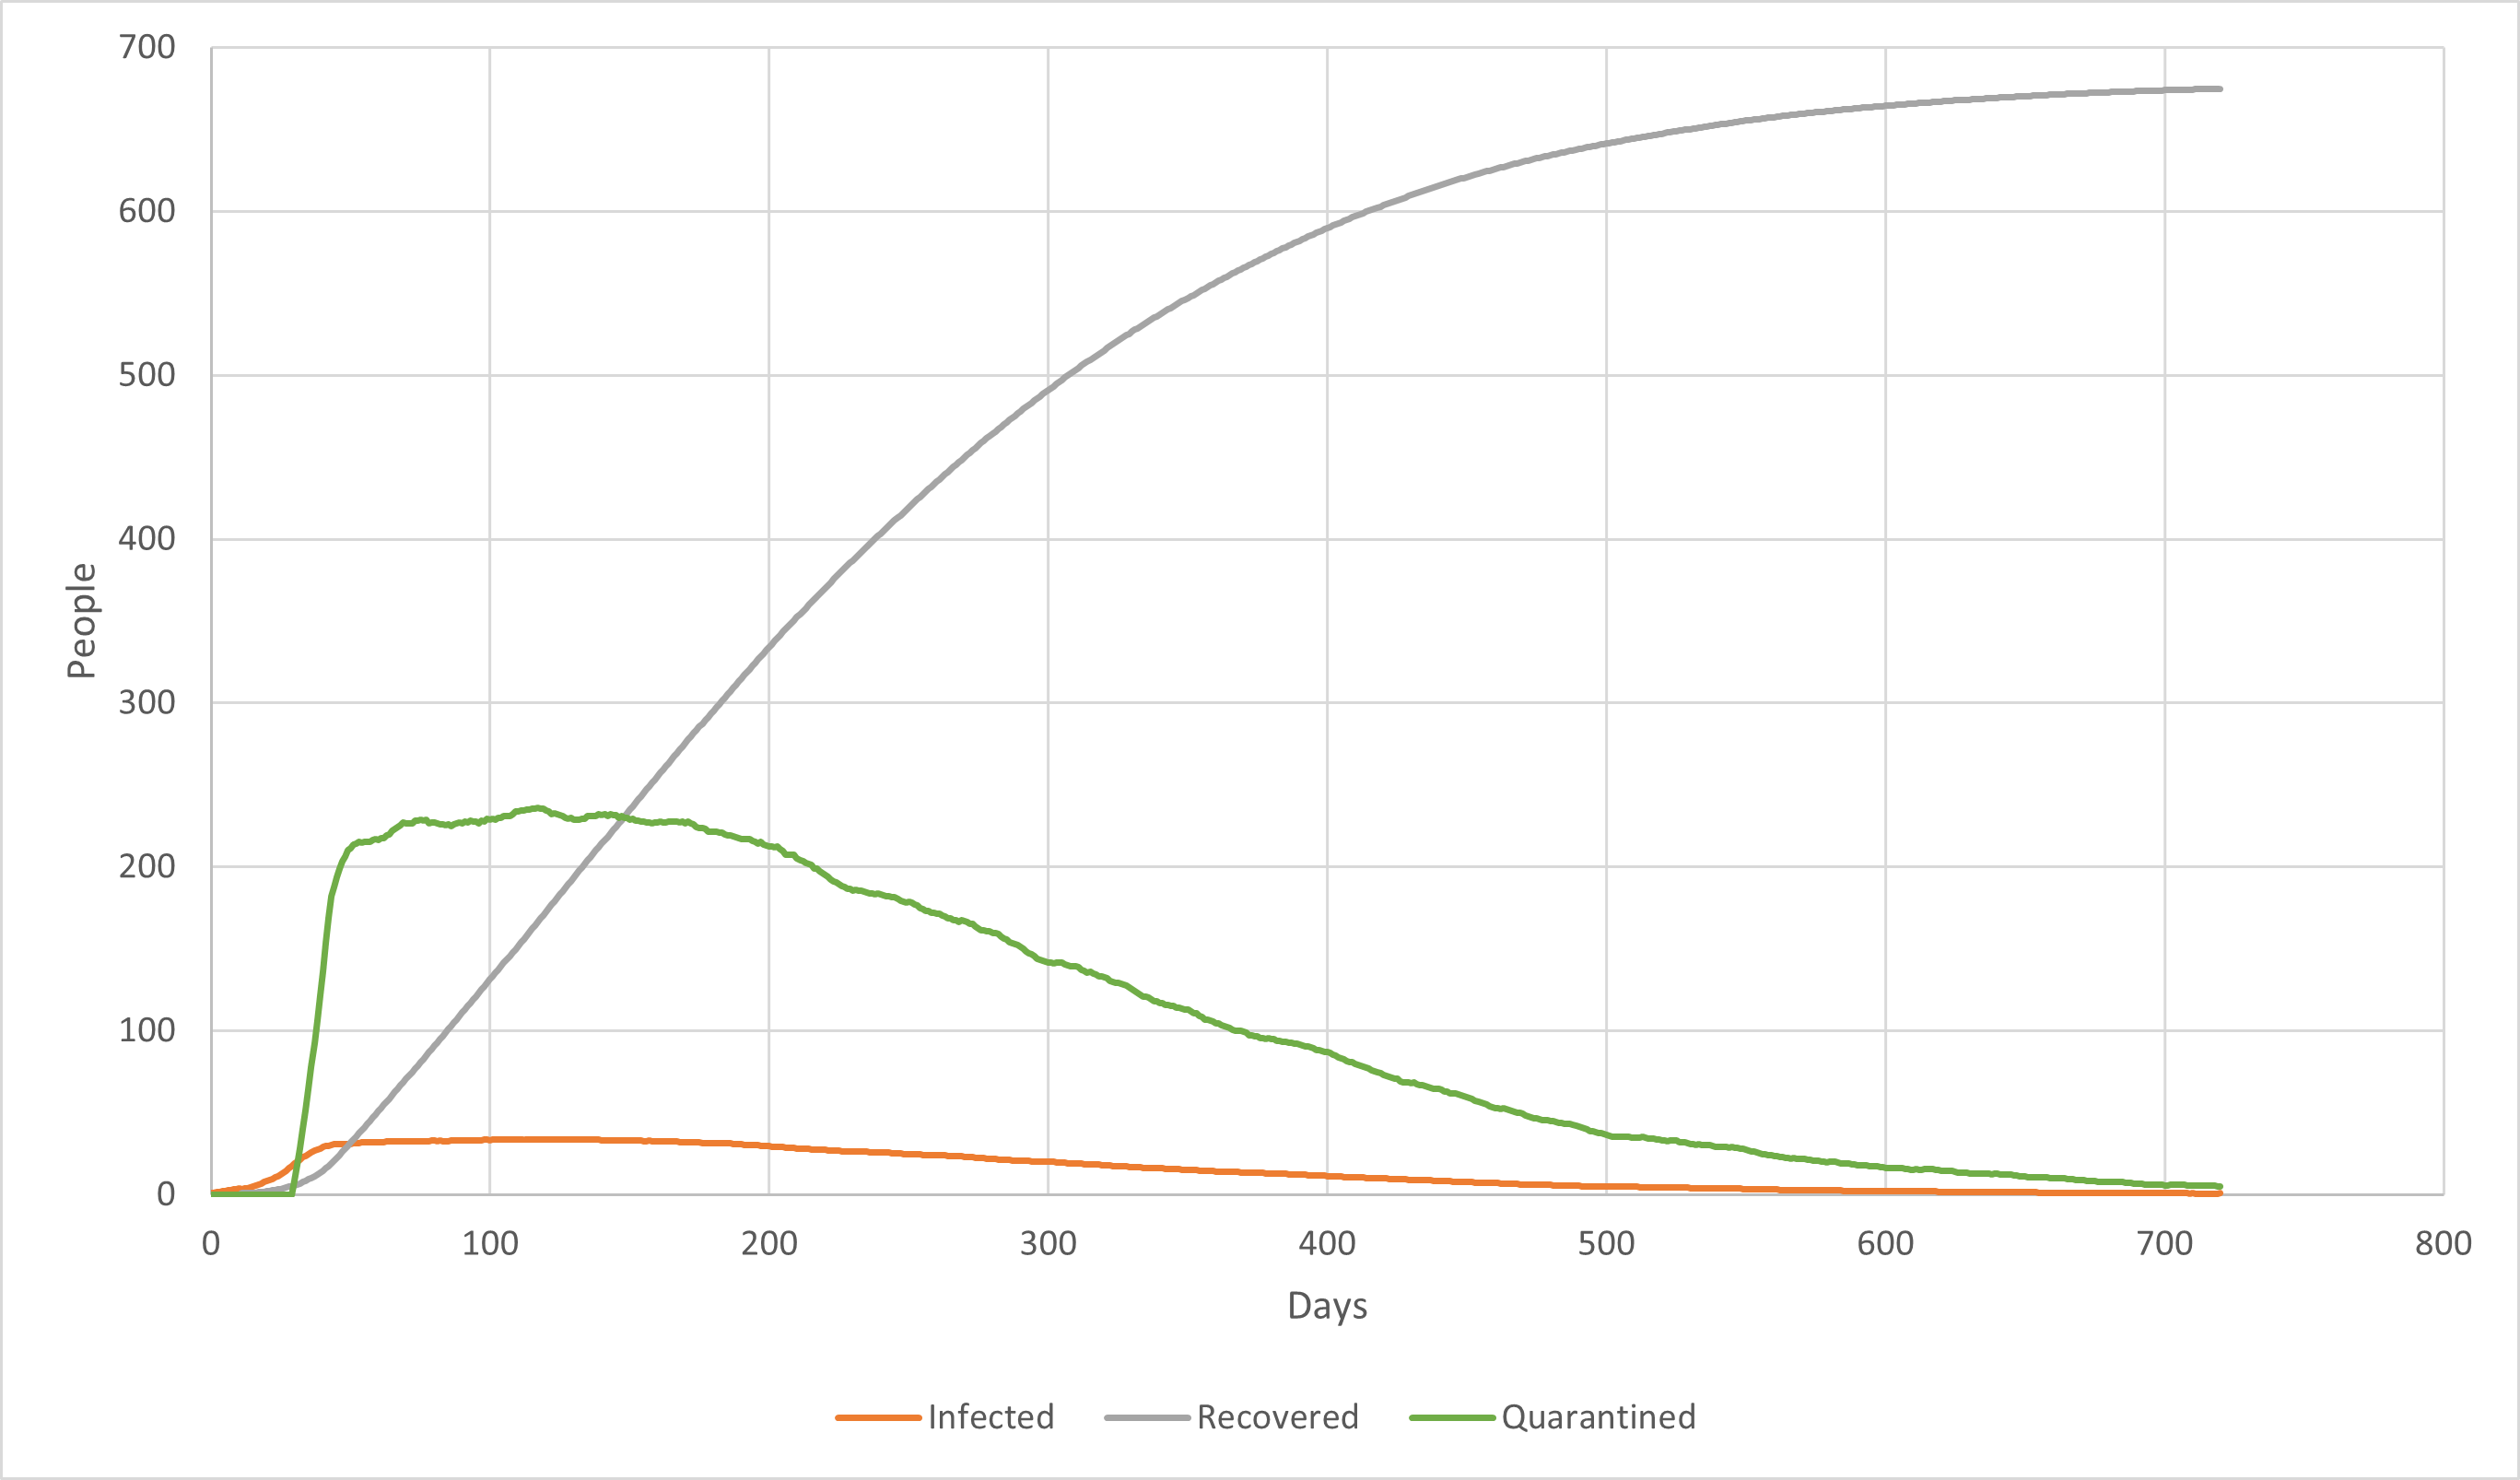
\includegraphics[width=0.75\textwidth]{0_billeder/Sim_CT_ON.png}
    \caption{Graph of quarantined, infected and recovered plotted against days, from simulation with contact tracing}
    \label{fig:Sim_CT_ON-1}
\end{figure}

In figure \ref{fig:Sim_CT_ON-1}, contact tracing has been enabled alongside quarantine. As is shown, this lengthens the infection period for the population as a whole, but greatly diminishes the number of infections across the population. 

Whereas there are about 900 recovered in the simulation run with no contact tracing (figure \ref{fig:Sim_CT_OFF-1}), there are under 700 recovered in the simulation run with contact tracing (figure \ref{fig:Sim_CT_ON-1}). This shows that contact tracing not only lowers the risk of infection to the individual person but also indicates a decrease in deaths (as these are grouped with recovered in the basic simulation).
\subsection{Comparative analyses of simulation results}

At the start of our different comparative analyses, we will first make a general rough analysis, creating a more simplified and easy-to-understand version of our results. As an example, in figure \ref{Fig:covidInfGraphs}, two histograms are visible, showcasing the only difference in the  simulation, namely the switching of contact tracing (CT). 

In the first histogram(a), the columns clearly show the effect of contact tracing. The maximum number of total infected within thousand drops of our simulation shows no higher than 210 infected of a total 12,500 population size, which equals to 1.68\% being infected of a total population. In other words, contact tracing seems to prove effective, since this is a very low total infection for the population. 

In the second histogram(b), the columns here shows a different reality. If COVID-19 were to run "invisibly", i.e. without society's knowledge and without the preventive measure of contact tracing, the simulation of a thousand drops estimates a maximum of 3857 infected. In comparison to histogram(a), in this simulation of thousand drops without contact tracing, the total infected population can reach as high as 30.8\% of the total population. 

\begin{figure}[H]
 \centering
  \begin{subfigure}{.45\textwidth}
    \centering
    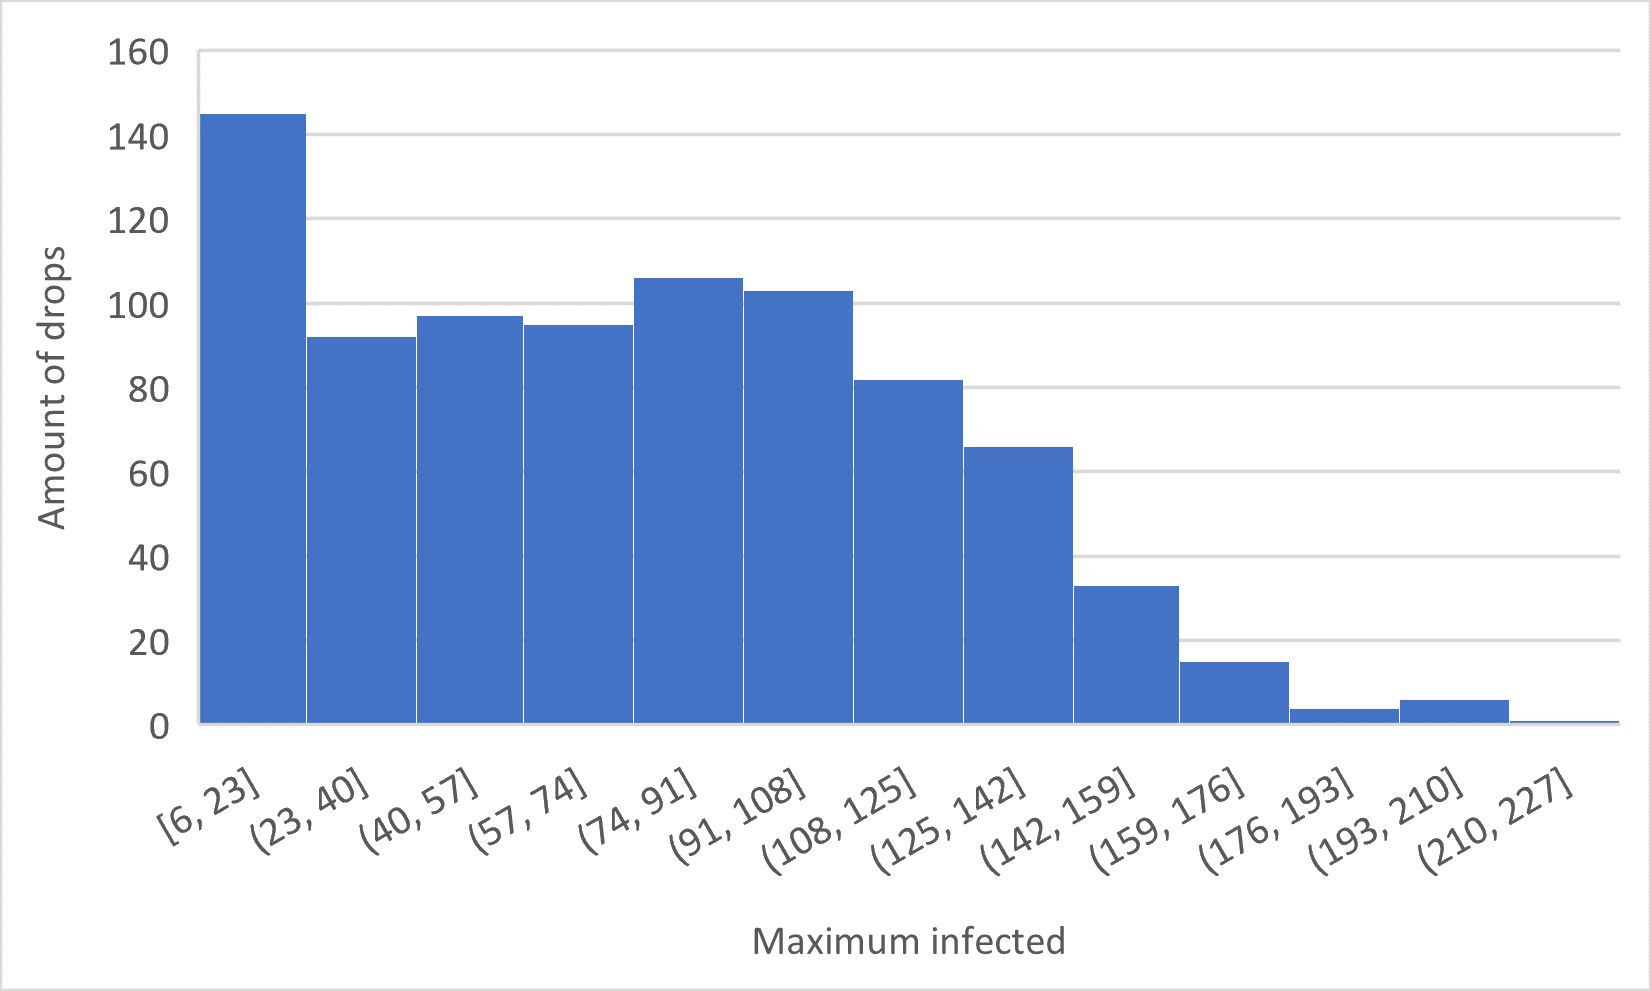
\includegraphics[width=.95\linewidth]{0_billeder/1k_ct_on_graph.png}
    \caption{With contact tracing}
    \label{Subfig:covidInfGraphA}
  \end{subfigure}
  \begin{subfigure}{.45\textwidth}
    \centering
    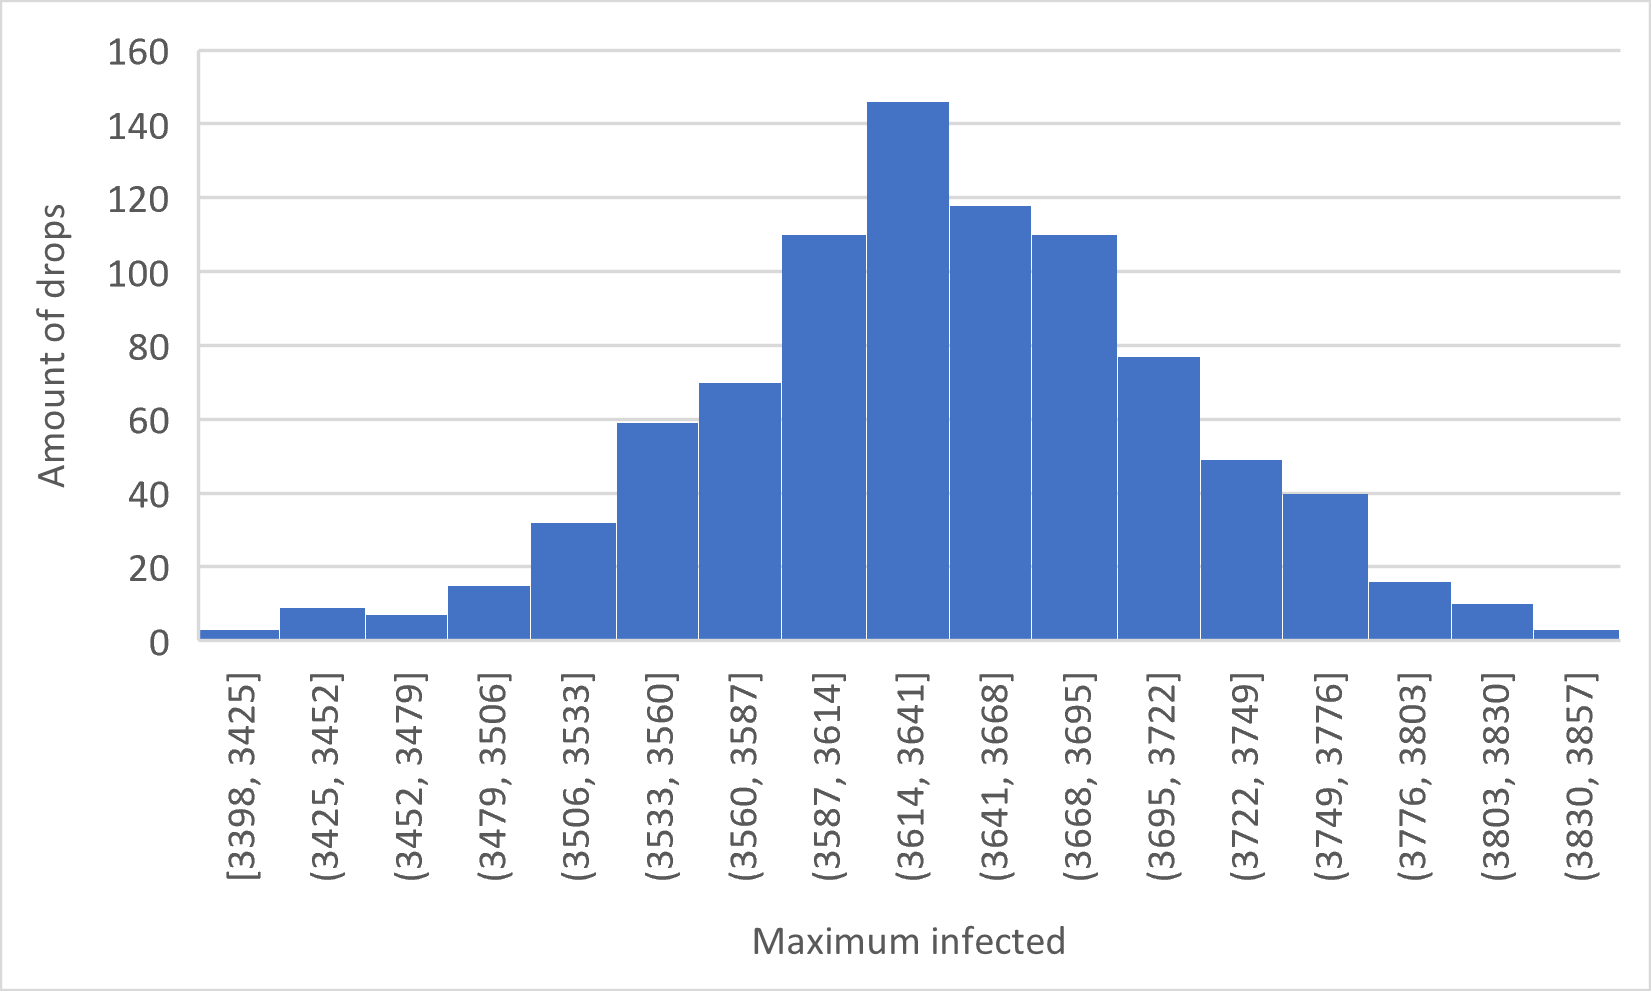
\includegraphics[width=.95\linewidth]{0_billeder/1k_ct_off_graph.png}
    \caption{Without contact tracing}
    \label{Subfig:covidInfGraphB}
  \end{subfigure}
 \caption{Infection histograms with/without contact tracing.}
 \label{Fig:covidInfGraphs}
\end{figure}

Figure \ref{Fig:covidInfGraphs} is a graph of infection, as a function of days, both with- and without contact tracing enabled. Before going into explaining the graphs, it is important to note, that the data used is an average of a thousand drops.

In the first graph with contact tracing disabled, we see that the number of infected people is raising rapidly to its peak which is around 2750 people infected - at day 112. Then the number of infected people quickly drops to 0 again around day 190 and do not change further.

In the second graph, which is with contact tracing enabled, the number of infected also raises rapidly, but it does not reach the same levels as in the first graph. The maximum number of infected in the second graph is around 33 at day 140. After it has peaked, it slowly decrease towards 0, which is reached around day 720.

Comparing the two, it is clear that contact tracing and quarantine is a very effective tool in fighting COVID-19. With contact tracing disabled, the number of infections peak at 2750 people, whereas with contact tracing enabled, it peaks at only 33 people. That corresponds to only 1.2\% of the first graph's peak.

\begin{figure}[H]
 \centering
  \begin{subfigure}{.45\textwidth}
    \centering
    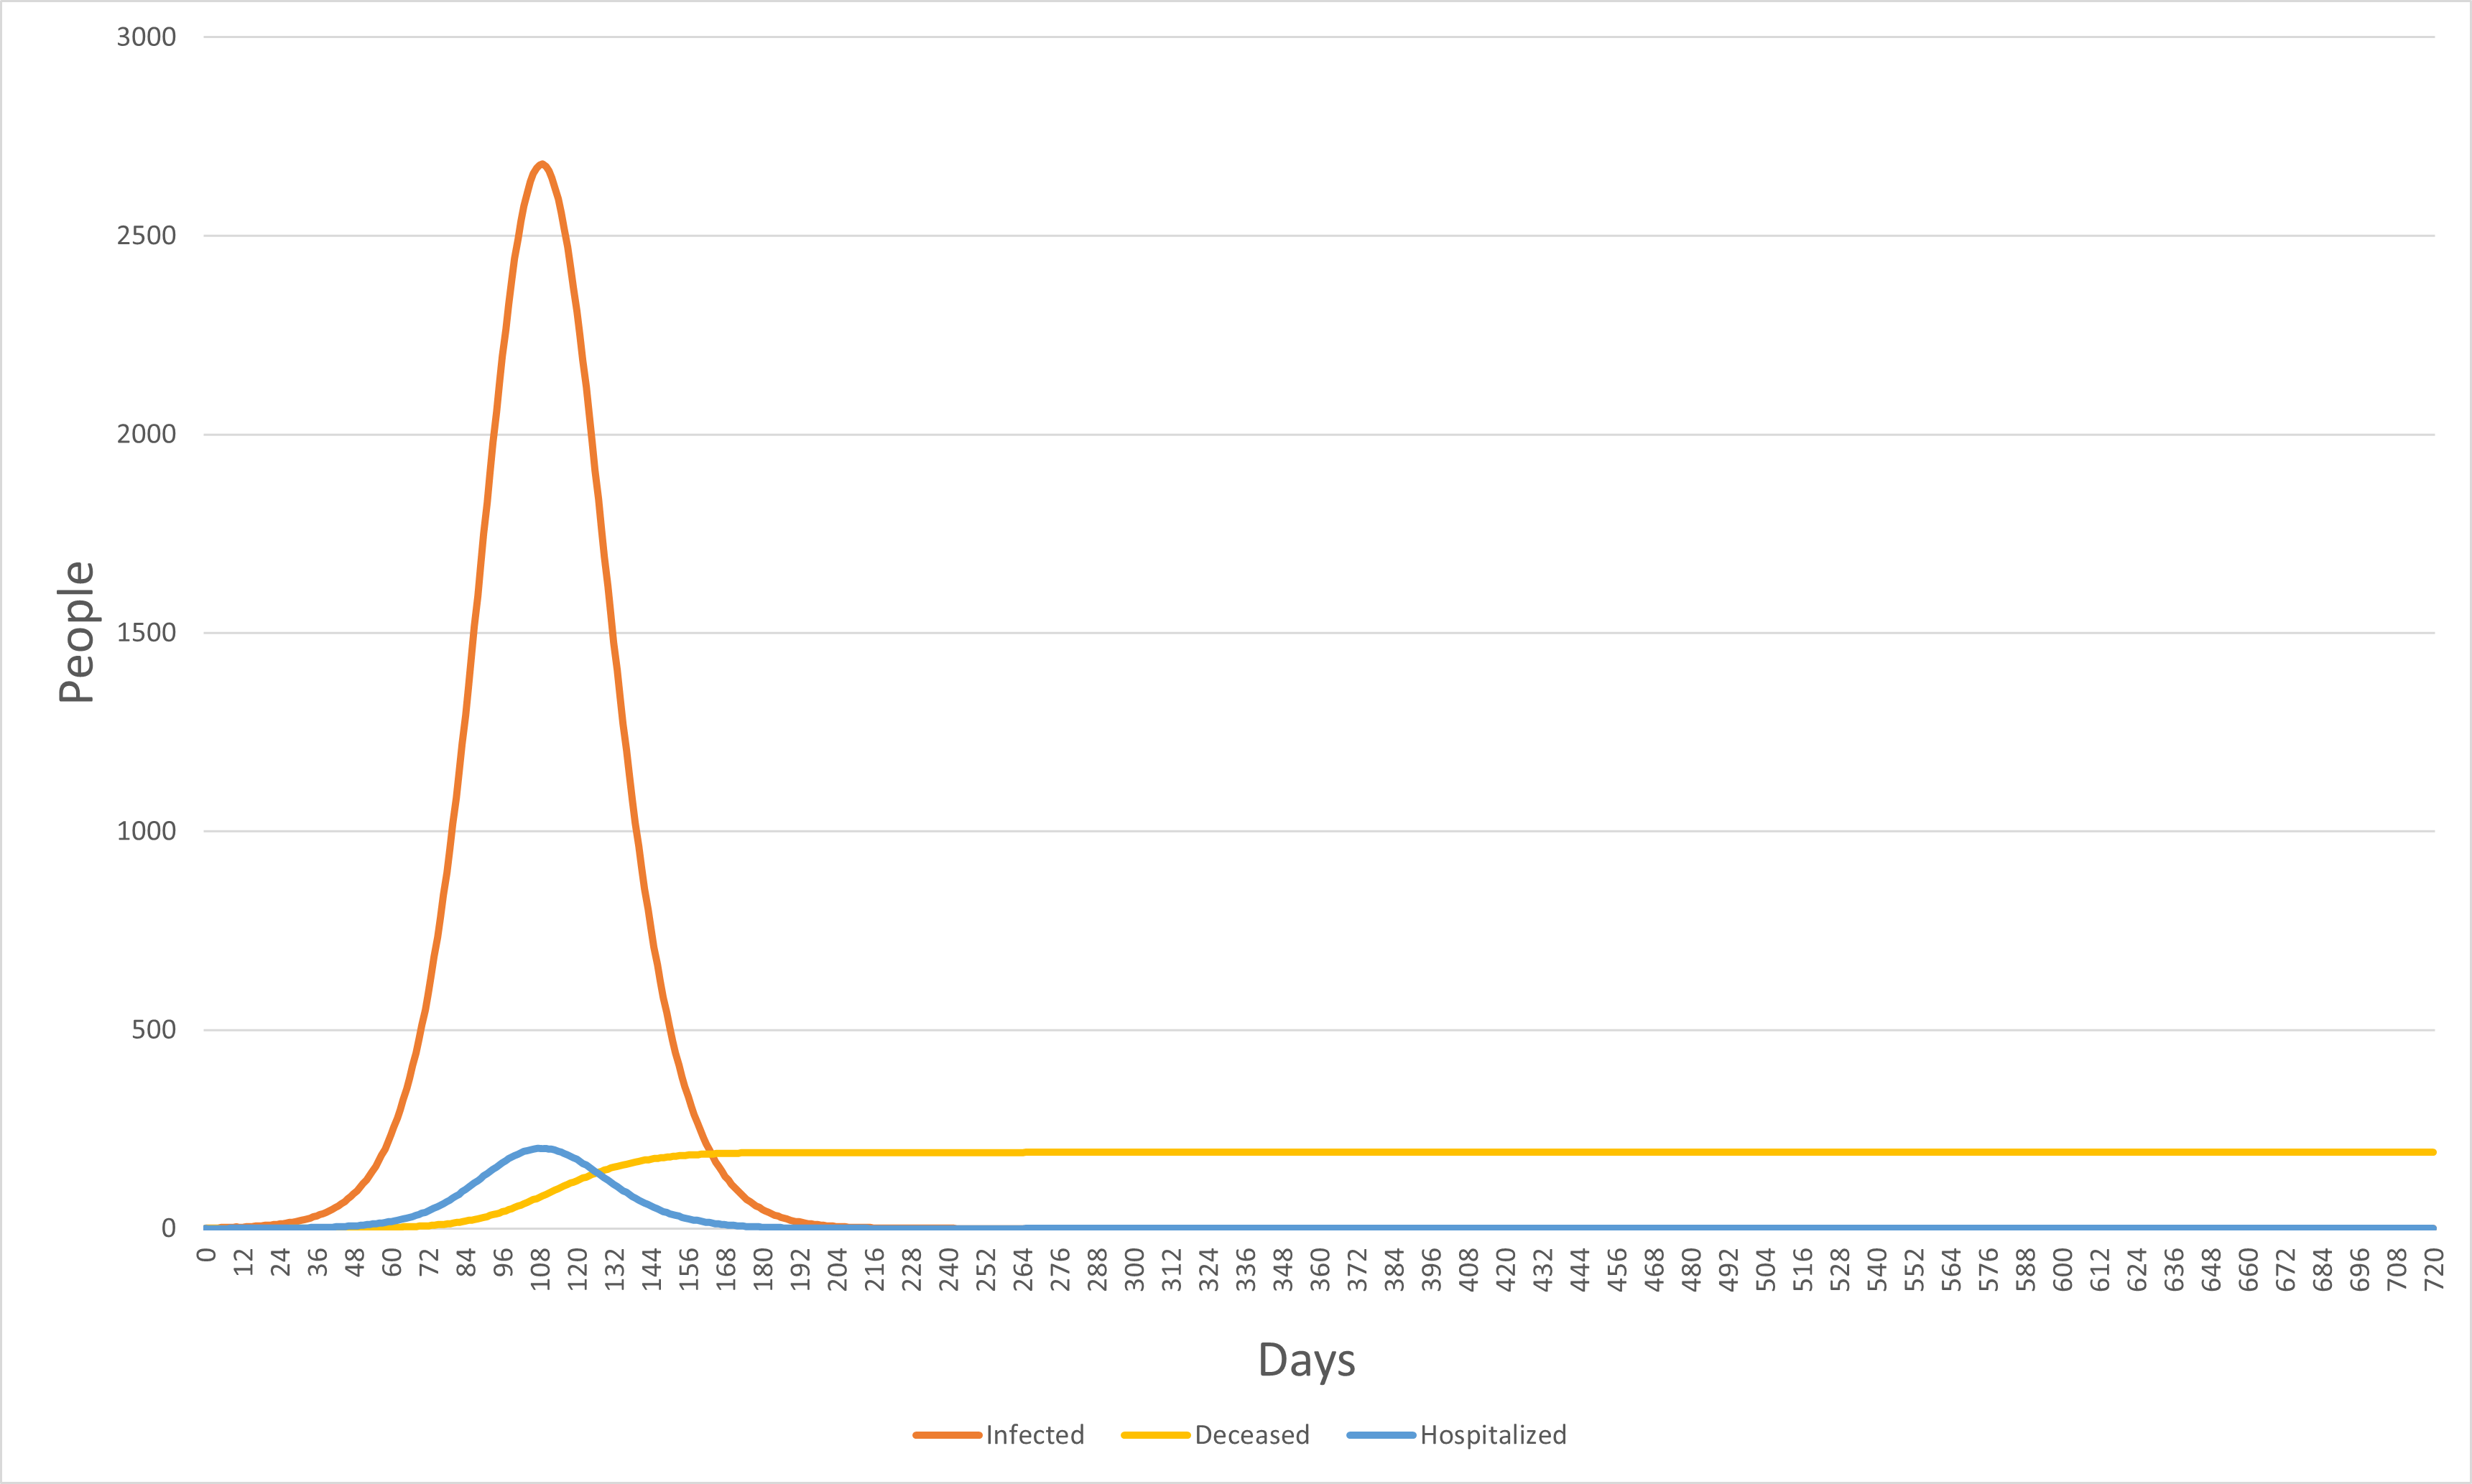
\includegraphics[width=.95\linewidth]{0_billeder/covidInfectionGraphA.png}
    \caption{With contact tracing}
    \label{Subfig:covidInfGraphA}
  \end{subfigure}
  \begin{subfigure}{.45\textwidth}
    \centering
    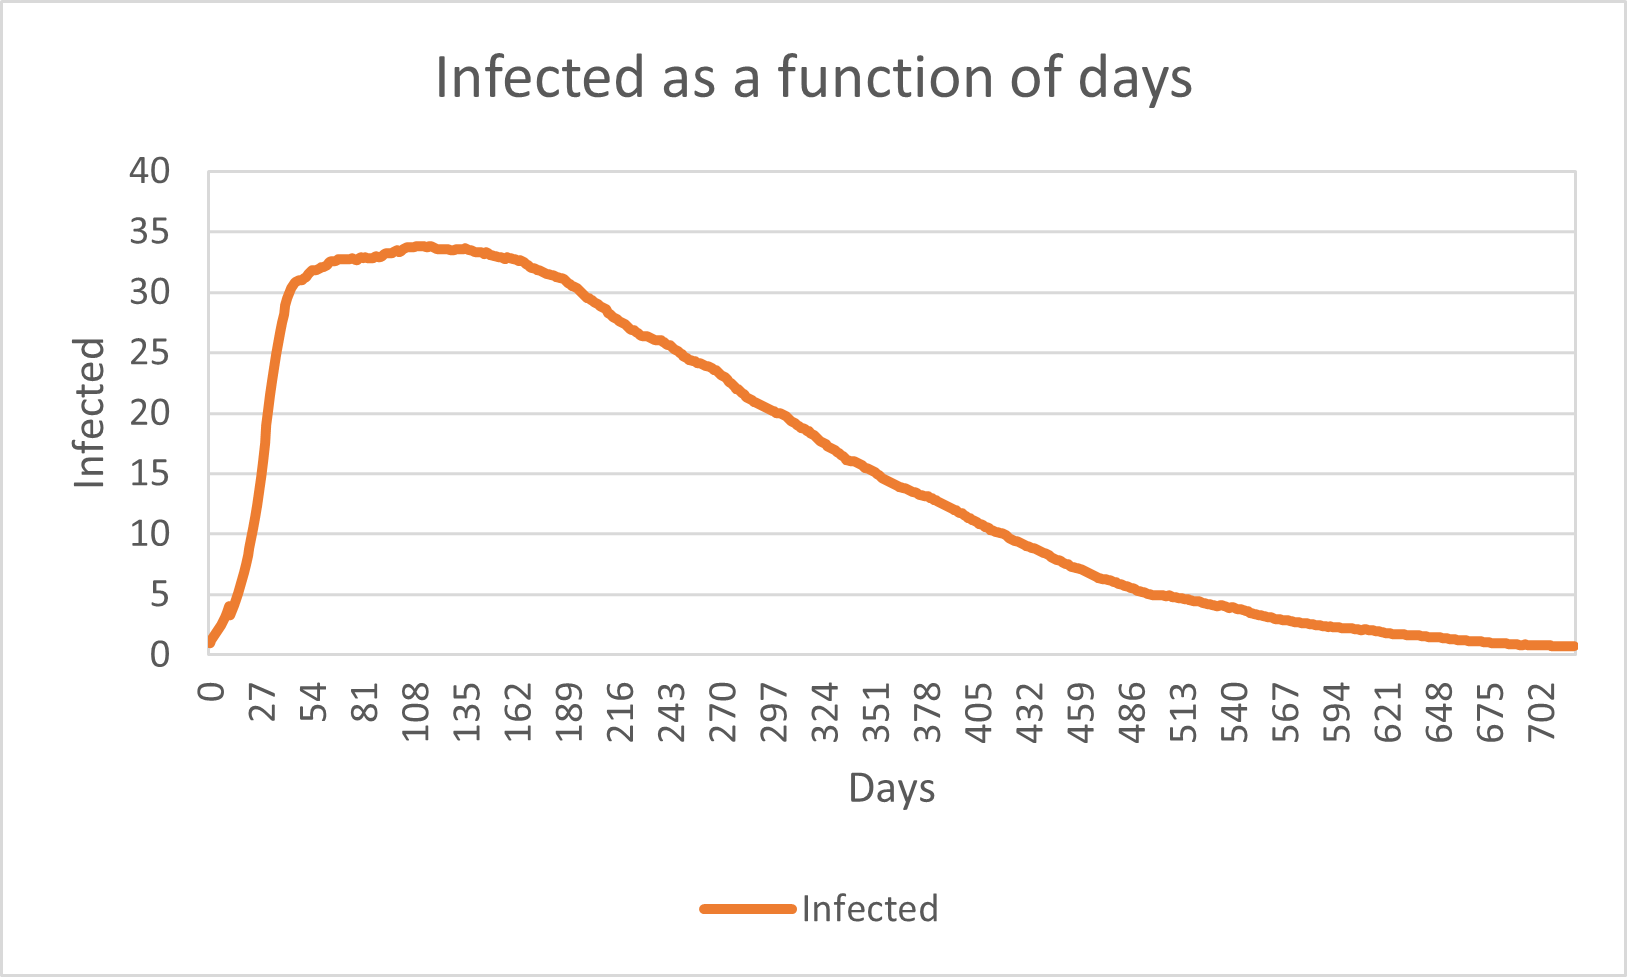
\includegraphics[width=.95\linewidth]{0_billeder/covidInfectionGraphB.png}
    \caption{Without contact tracing}
    \label{Subfig:covidInfGraphB}
  \end{subfigure}
 \caption{Infection graphs with and without contact tracing.}
 \label{Fig:covidInfGraphs}
\end{figure}

\section{Sensitivity Study}
A sensitivity study is done to get a better understanding of how different parameters of our contact tracing implementation affects the simulation. We have chosen to change the day we start the tracing, the quarantine period and the amount of traceable contacts. To see how these affect the effectiveness of contact tracing in the simulation. Only one variable will be changed at a time to ensure that we know exactly how a specific variable had an effect.

The base settings for our simulation is that the starting time for CT is set to 30 days, the number of contacts a person has each day is 10, the tracing of contacts goes 2 days back, the quarantine period for traced contacts is 14 days and the number of contacts that can be traced is a random number between 5 and 20. 

\subsection{Tracing start time}
Our standard start time for contact tracing we have set in our simulation is 30 days, in this section we will look at the effects it would have if it started earlier and later, for this we have tried to run the simulation with a start time of 15 and 60 days respectively. In the next couple of graphs we will see how this has an effect on the number of infected as well as the number of people put in quarantine.

\begin{figure}[H]
\centering
\begin{subfigure}{.5\textwidth}
  \centering
  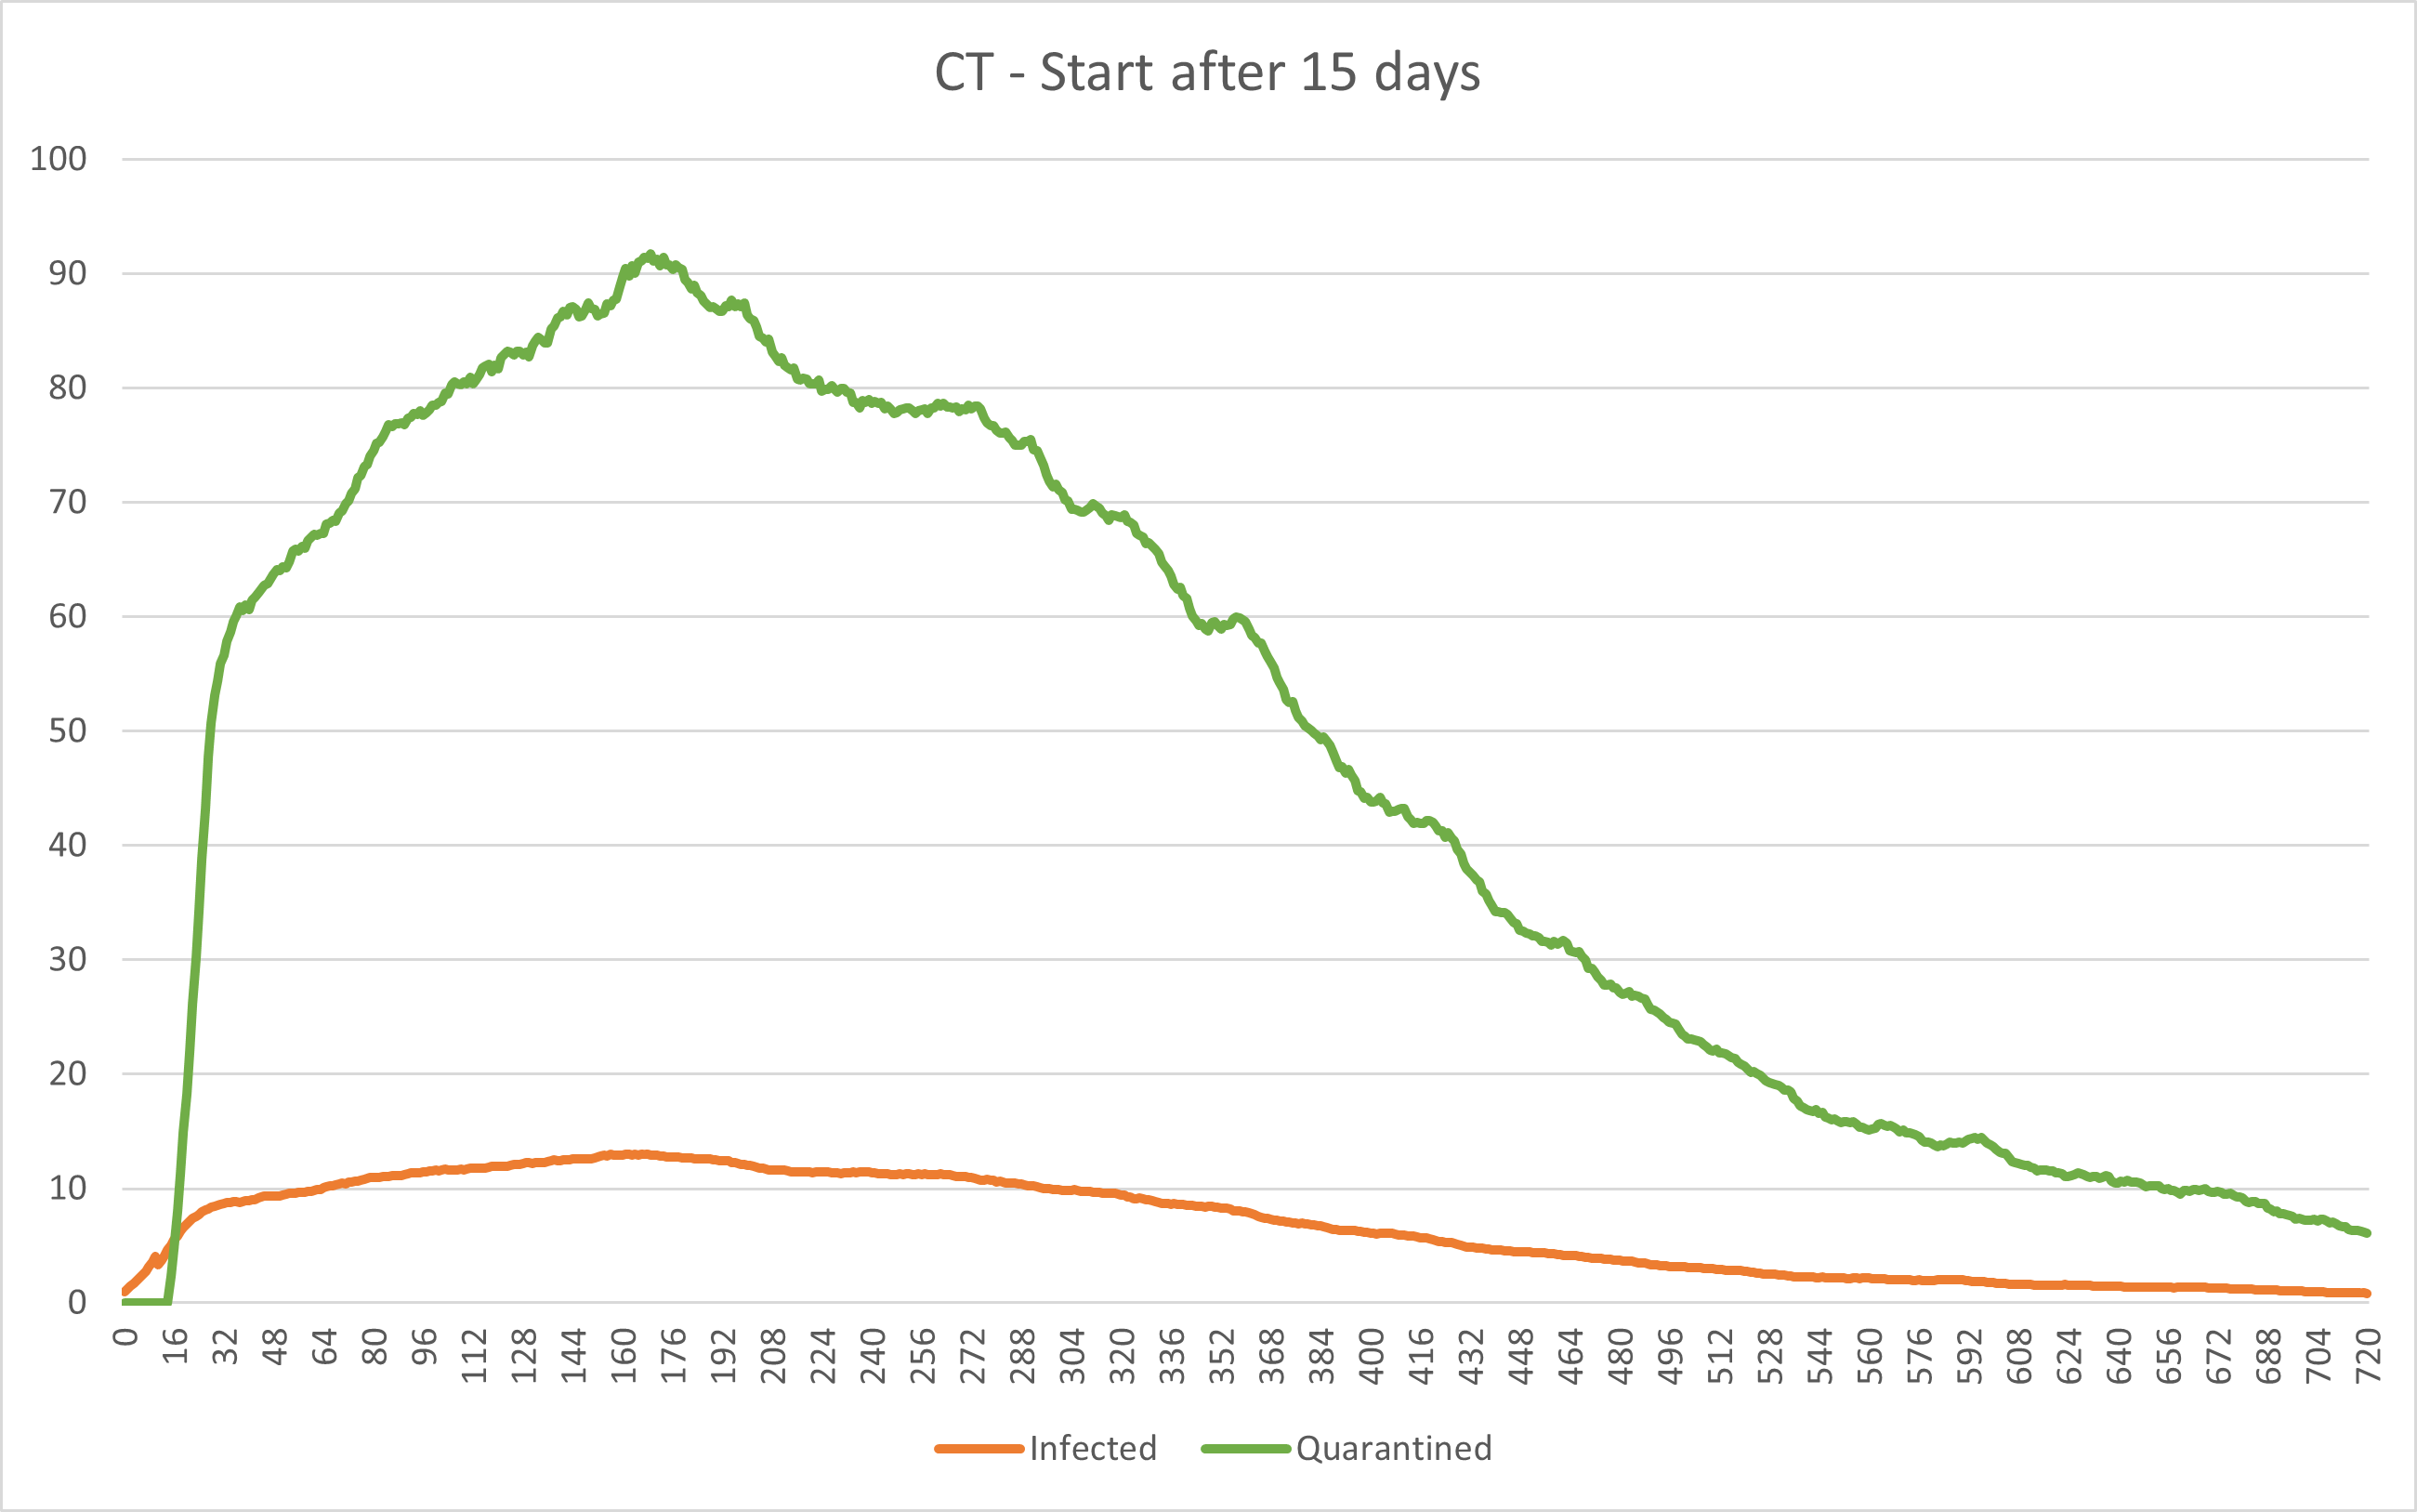
\includegraphics[width=.95\linewidth]{0_billeder/CT15Days.png}
  \caption{Contact tracing starting after 15 days}
  \label{Subfig:CT15}
\end{subfigure}%
\begin{subfigure}{.5\textwidth}
  \centering
  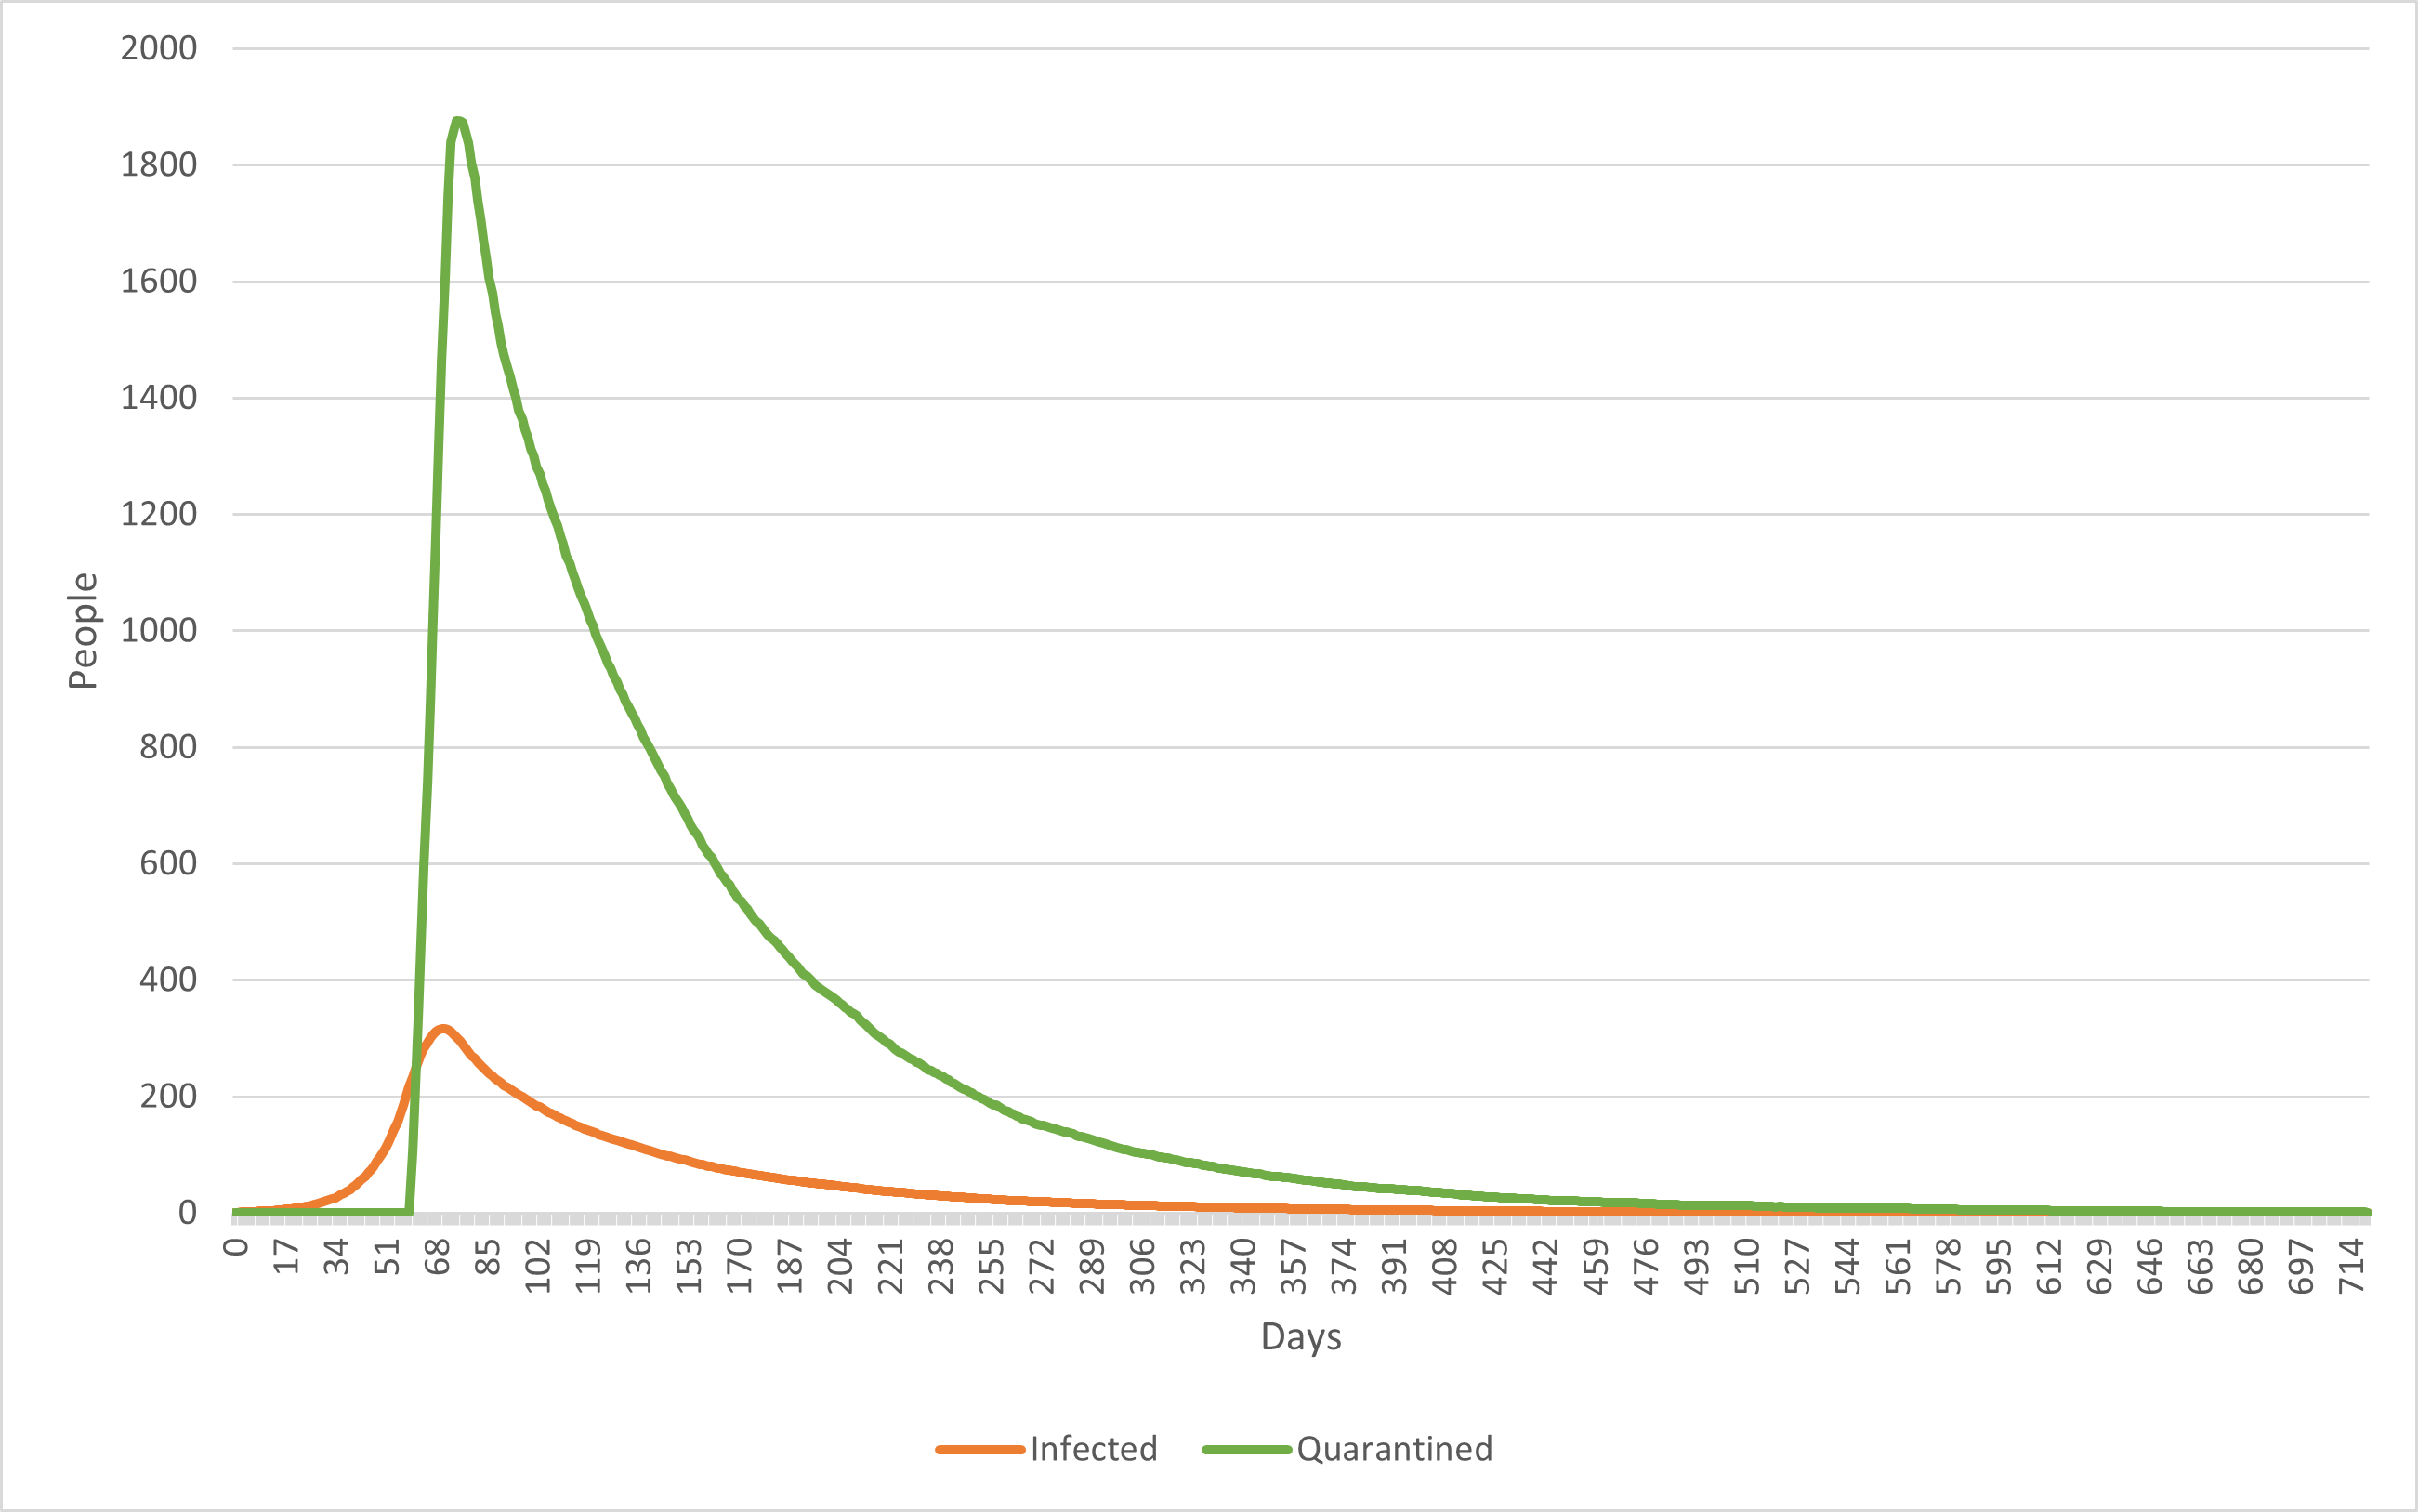
\includegraphics[width=.95\linewidth]{0_billeder/CT60Days.png}
  \caption{Contact tracing starting after 60 days}
  \label{Subfig:CT60}
\end{subfigure}
\caption{Graphs for number of people quarantined and infected plottet against days (Be aware of different proportions on the y-axis)}
\label{fig:CTstart1}
\end{figure}
From these graphs on figure \ref{fig:CTstart1} it can be seen that when we start tracing contacts in the population has a huge impact on both how many contacts that needs to be traced in total, as well as how many people become infected. It should also be noted that our simulation uses a much more \say{perfect} form of contact tracing, where everybody is at least able to trace 5 of their contacts over the previous 2 days. This is also the reason we see such a huge spike in the number of people quarantined when we reach the start time, since somewhere between 5-20 times the number of infected who are not asymptomatic and not in incubation will be quarantined.

It is also interesting to see that the early start in figure \ref{Subfig:CT15} results in a much more steady number of infected and a slow decline when its compared to the much later start on CT in figure \ref{Subfig:CT60}. This indicates that the earlier we start contact tracing the lower the amount of people who get infected and a substantial lower amount of the population needs to be traced.

\begin{figure}[H]
\centering
\begin{subfigure}{.5\textwidth}
  \centering
  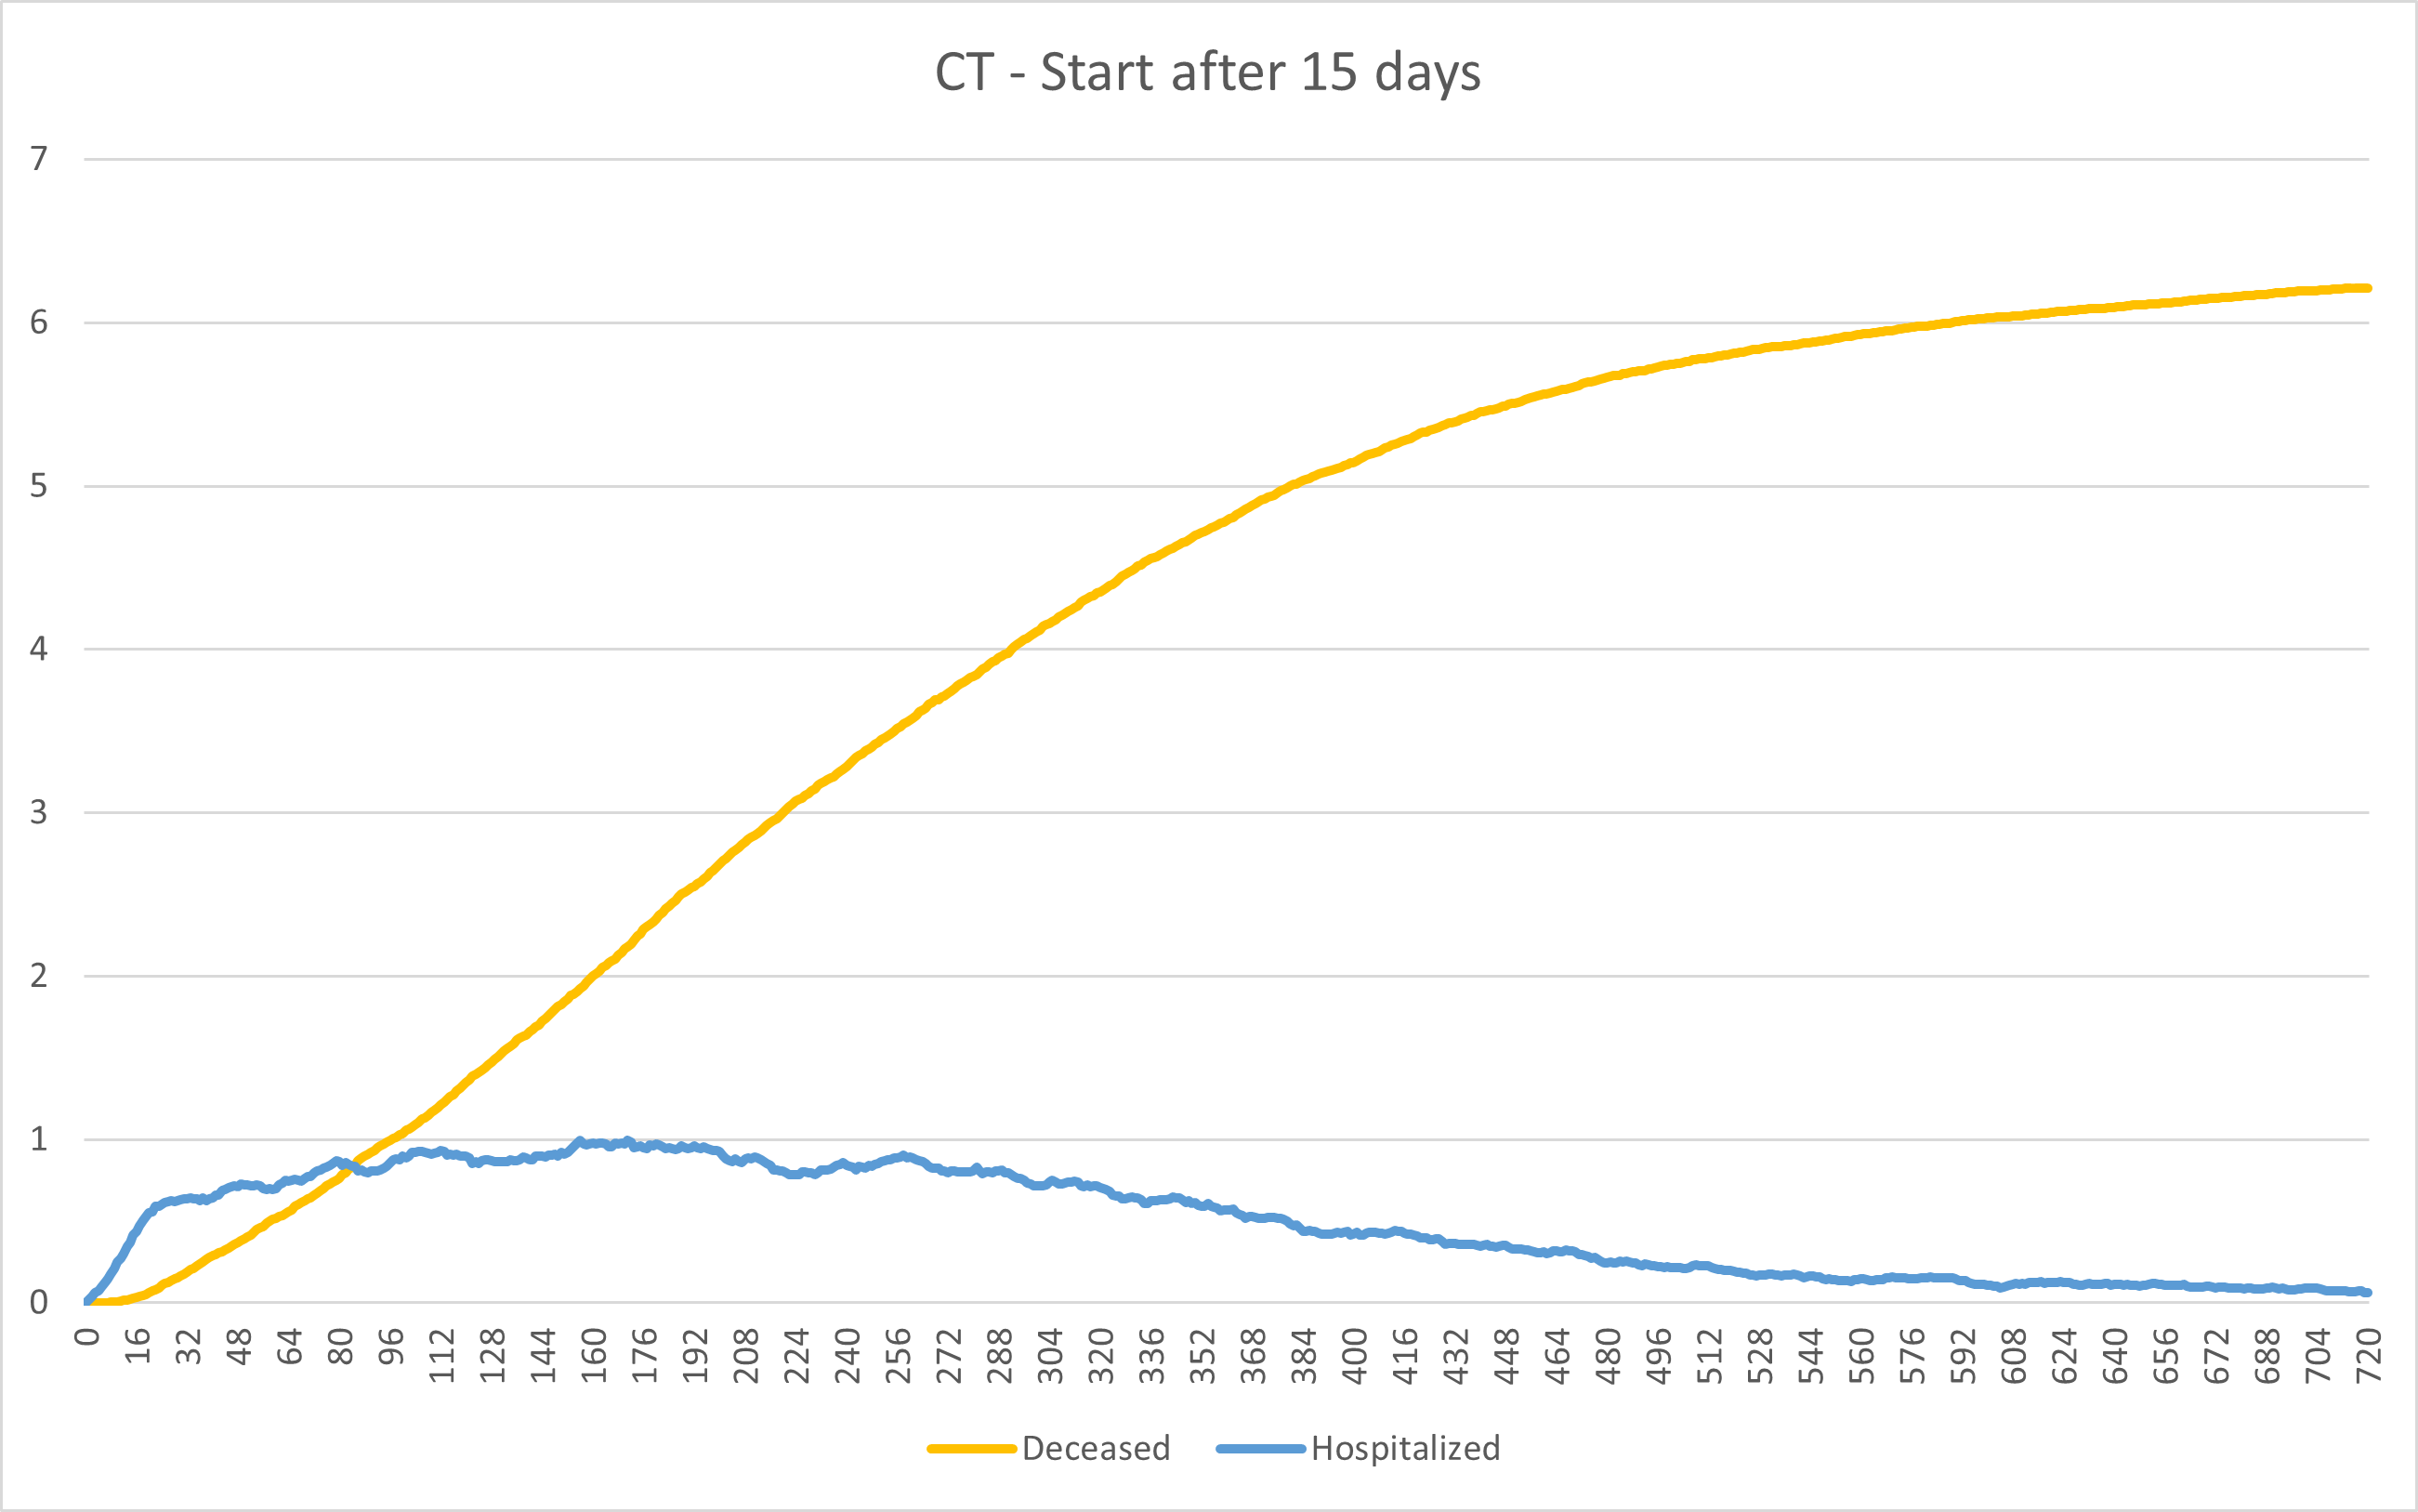
\includegraphics[width=.95\linewidth]{0_billeder/CT15DaysDH.png}
  \caption{Contact tracing starting after 15 days}
  \label{Subfig:CT15DH}
\end{subfigure}%
\begin{subfigure}{.5\textwidth}
  \centering
  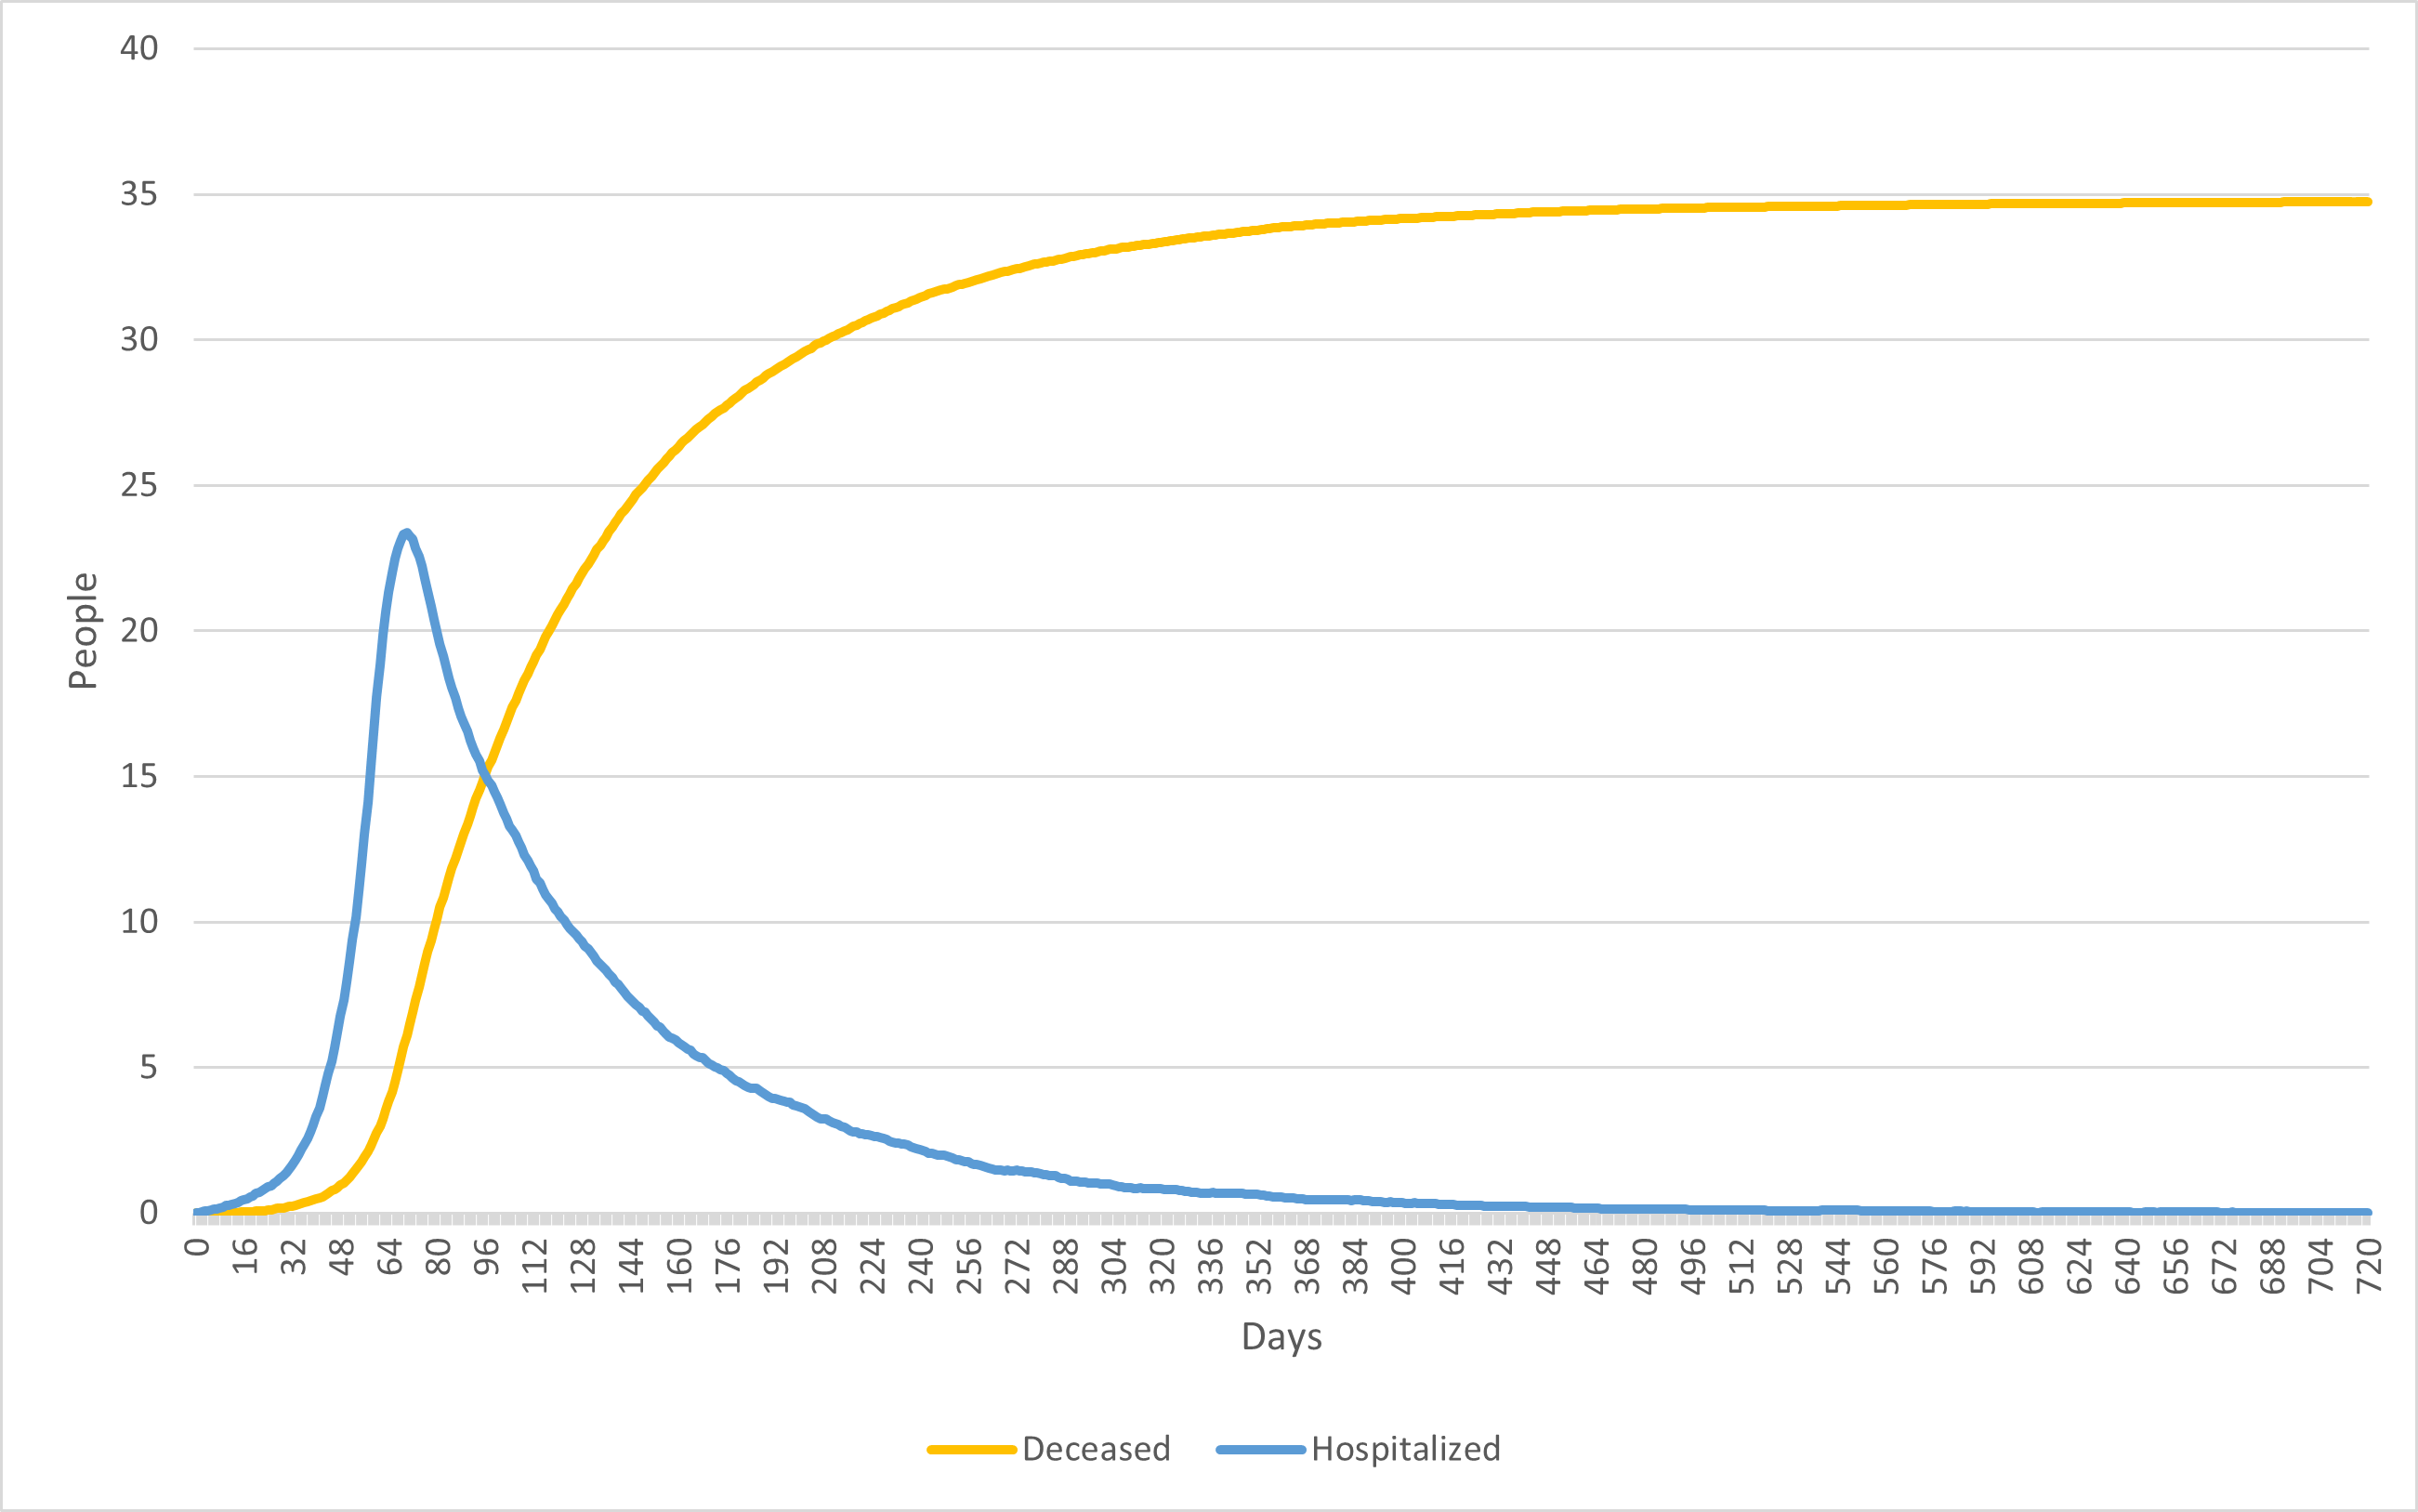
\includegraphics[width=.95\linewidth]{0_billeder/CT60DaysDH.png}
  \caption{Contact tracing starting after 60 days}
  \label{Subfig:CT60DH}
\end{subfigure}
\caption{Graphs for number of people hospitalized and deceased plottet against days (Be aware of different proportions on the y-axis)}
\label{fig:CTstart2}
\end{figure}

Since the starting time had such a notable effect on the number of people who became infected, it also had very big impact on the 


\subsection{Quarantine Period}
In this section we are looking at how the quarantine period will affect the amount of persons getting infected. We have run a simulation with a quarantine period of 7 day and one with 21 days. The two graphs below show how the two quarantine periods affect the amount people getting infected and are put into quarantine.


\begin{figure}[H]
\centering
\begin{subfigure}{.5\textwidth}
  \centering
  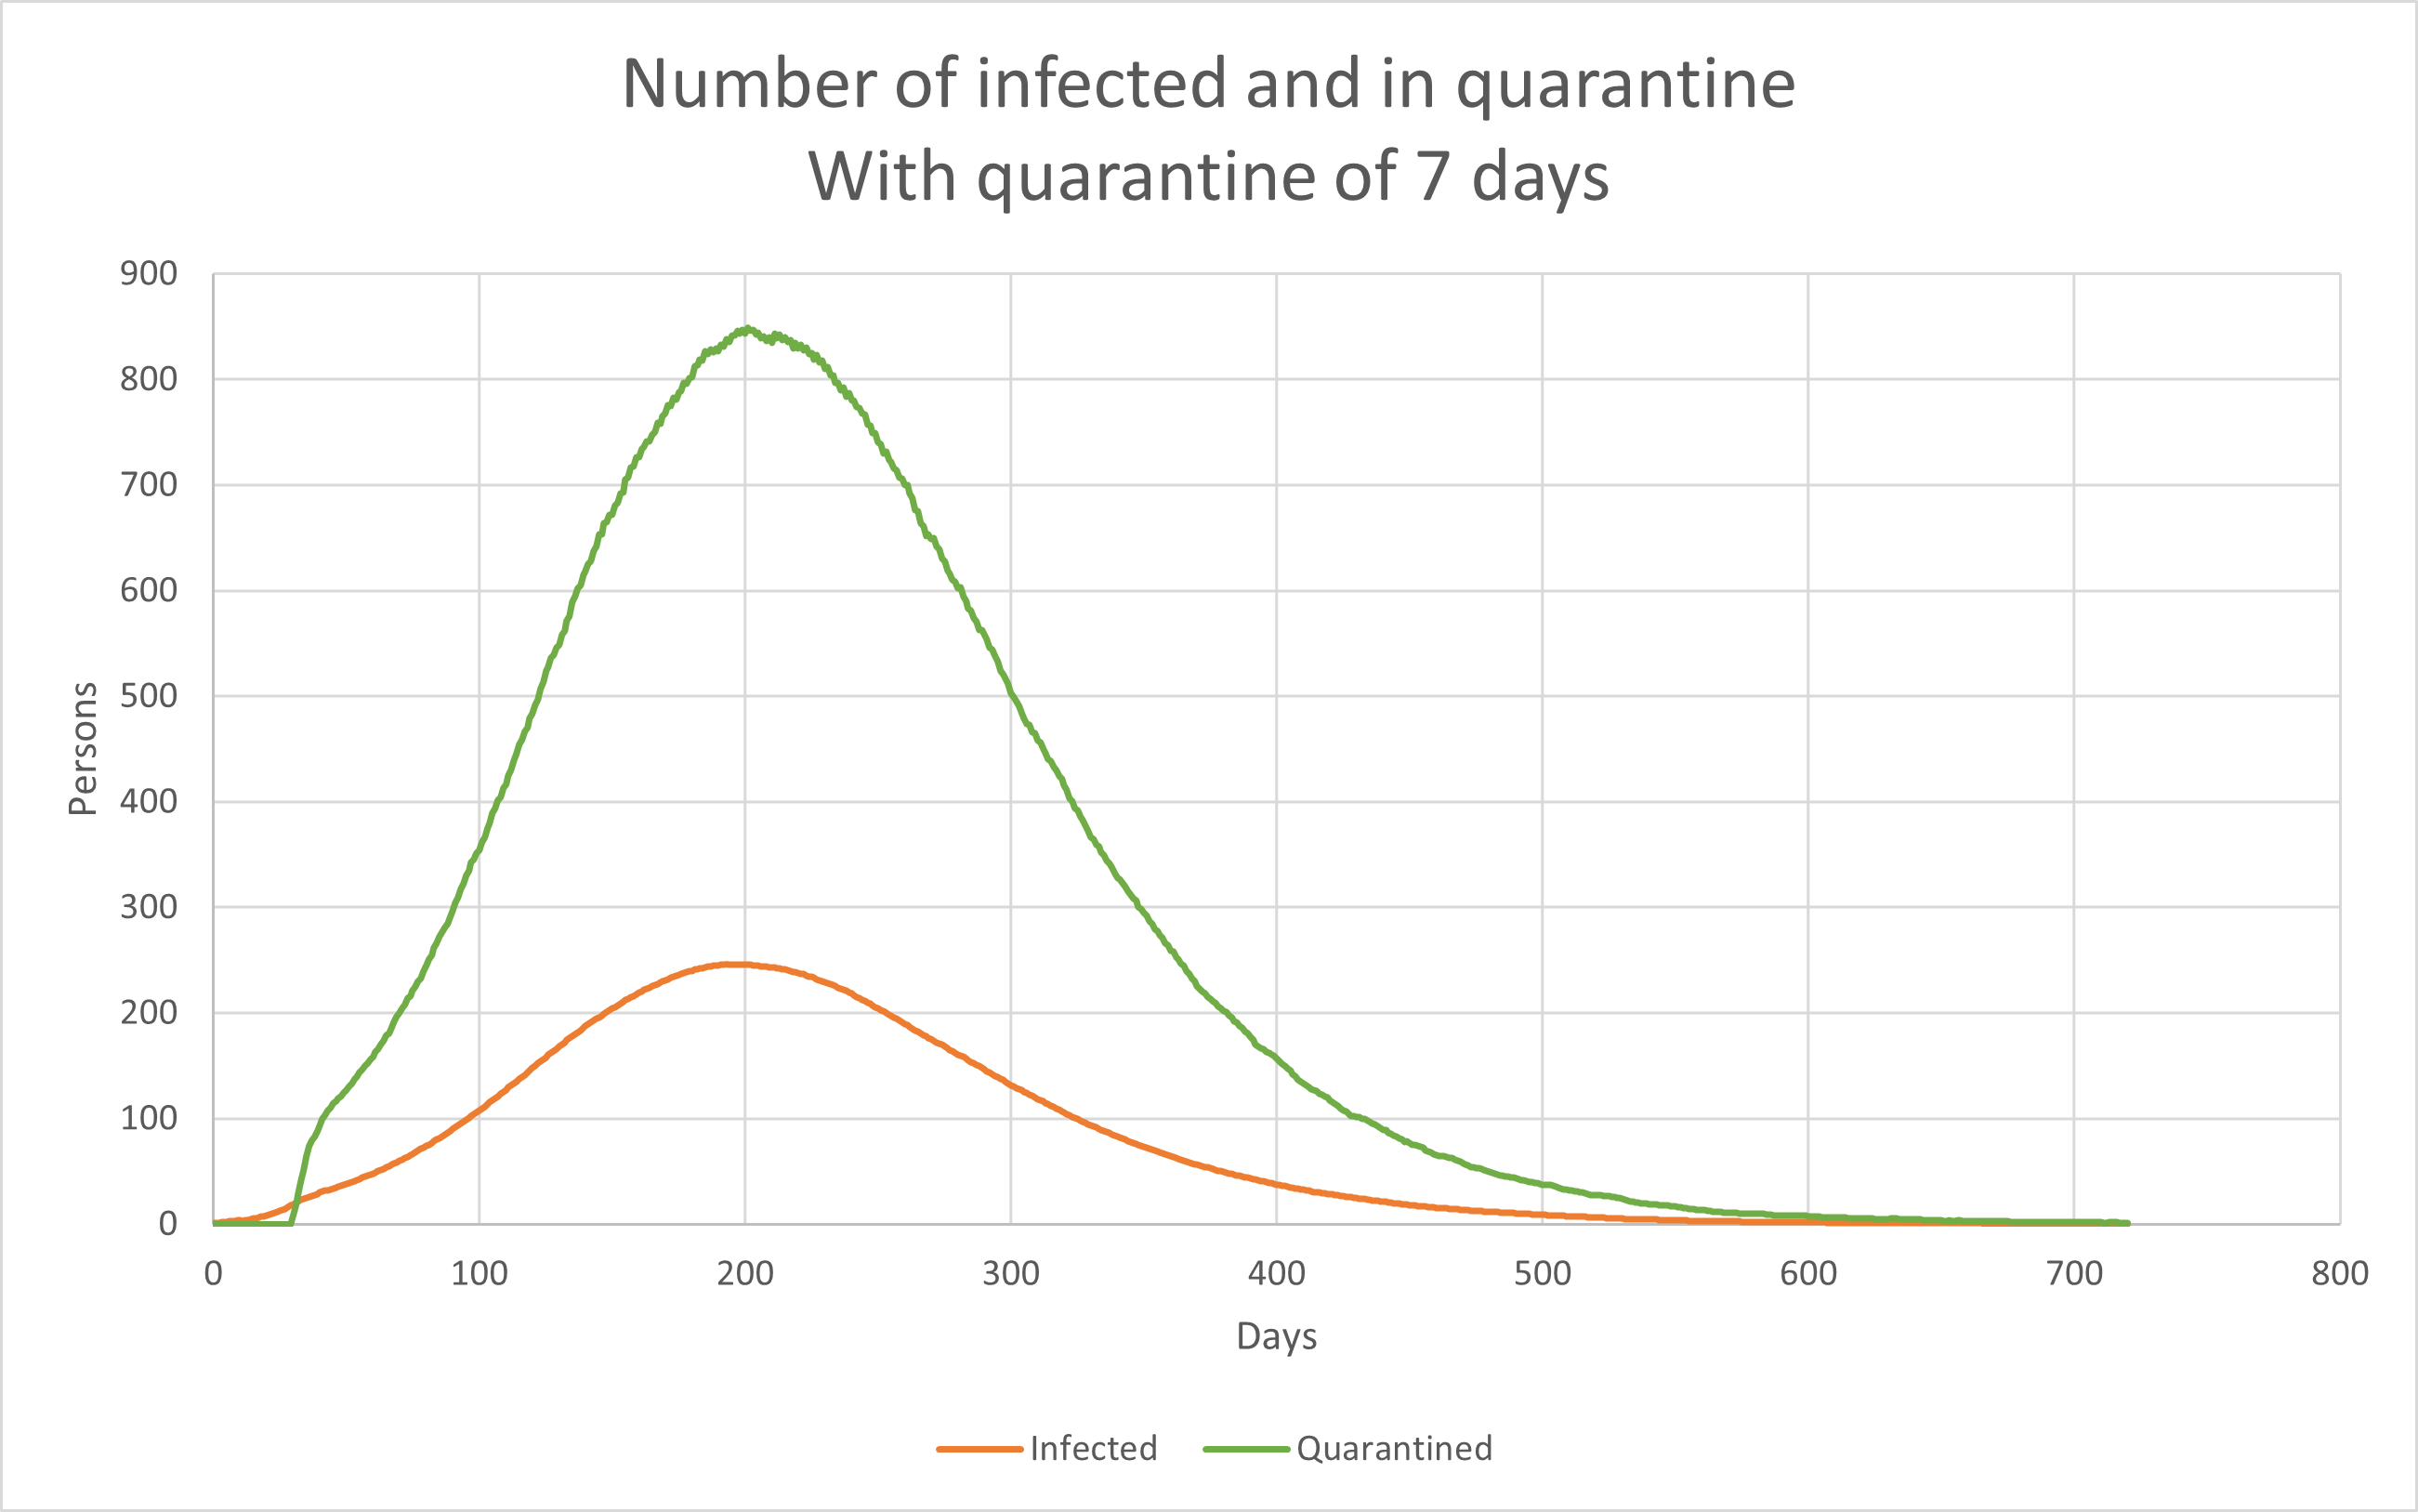
\includegraphics[width=.95\linewidth]{0_billeder/CT_Q_7.png}
  \caption{Quarantine period of 7 days}
  \label{fig:sub1}
\end{subfigure}%
\begin{subfigure}{.5\textwidth}
  \centering
  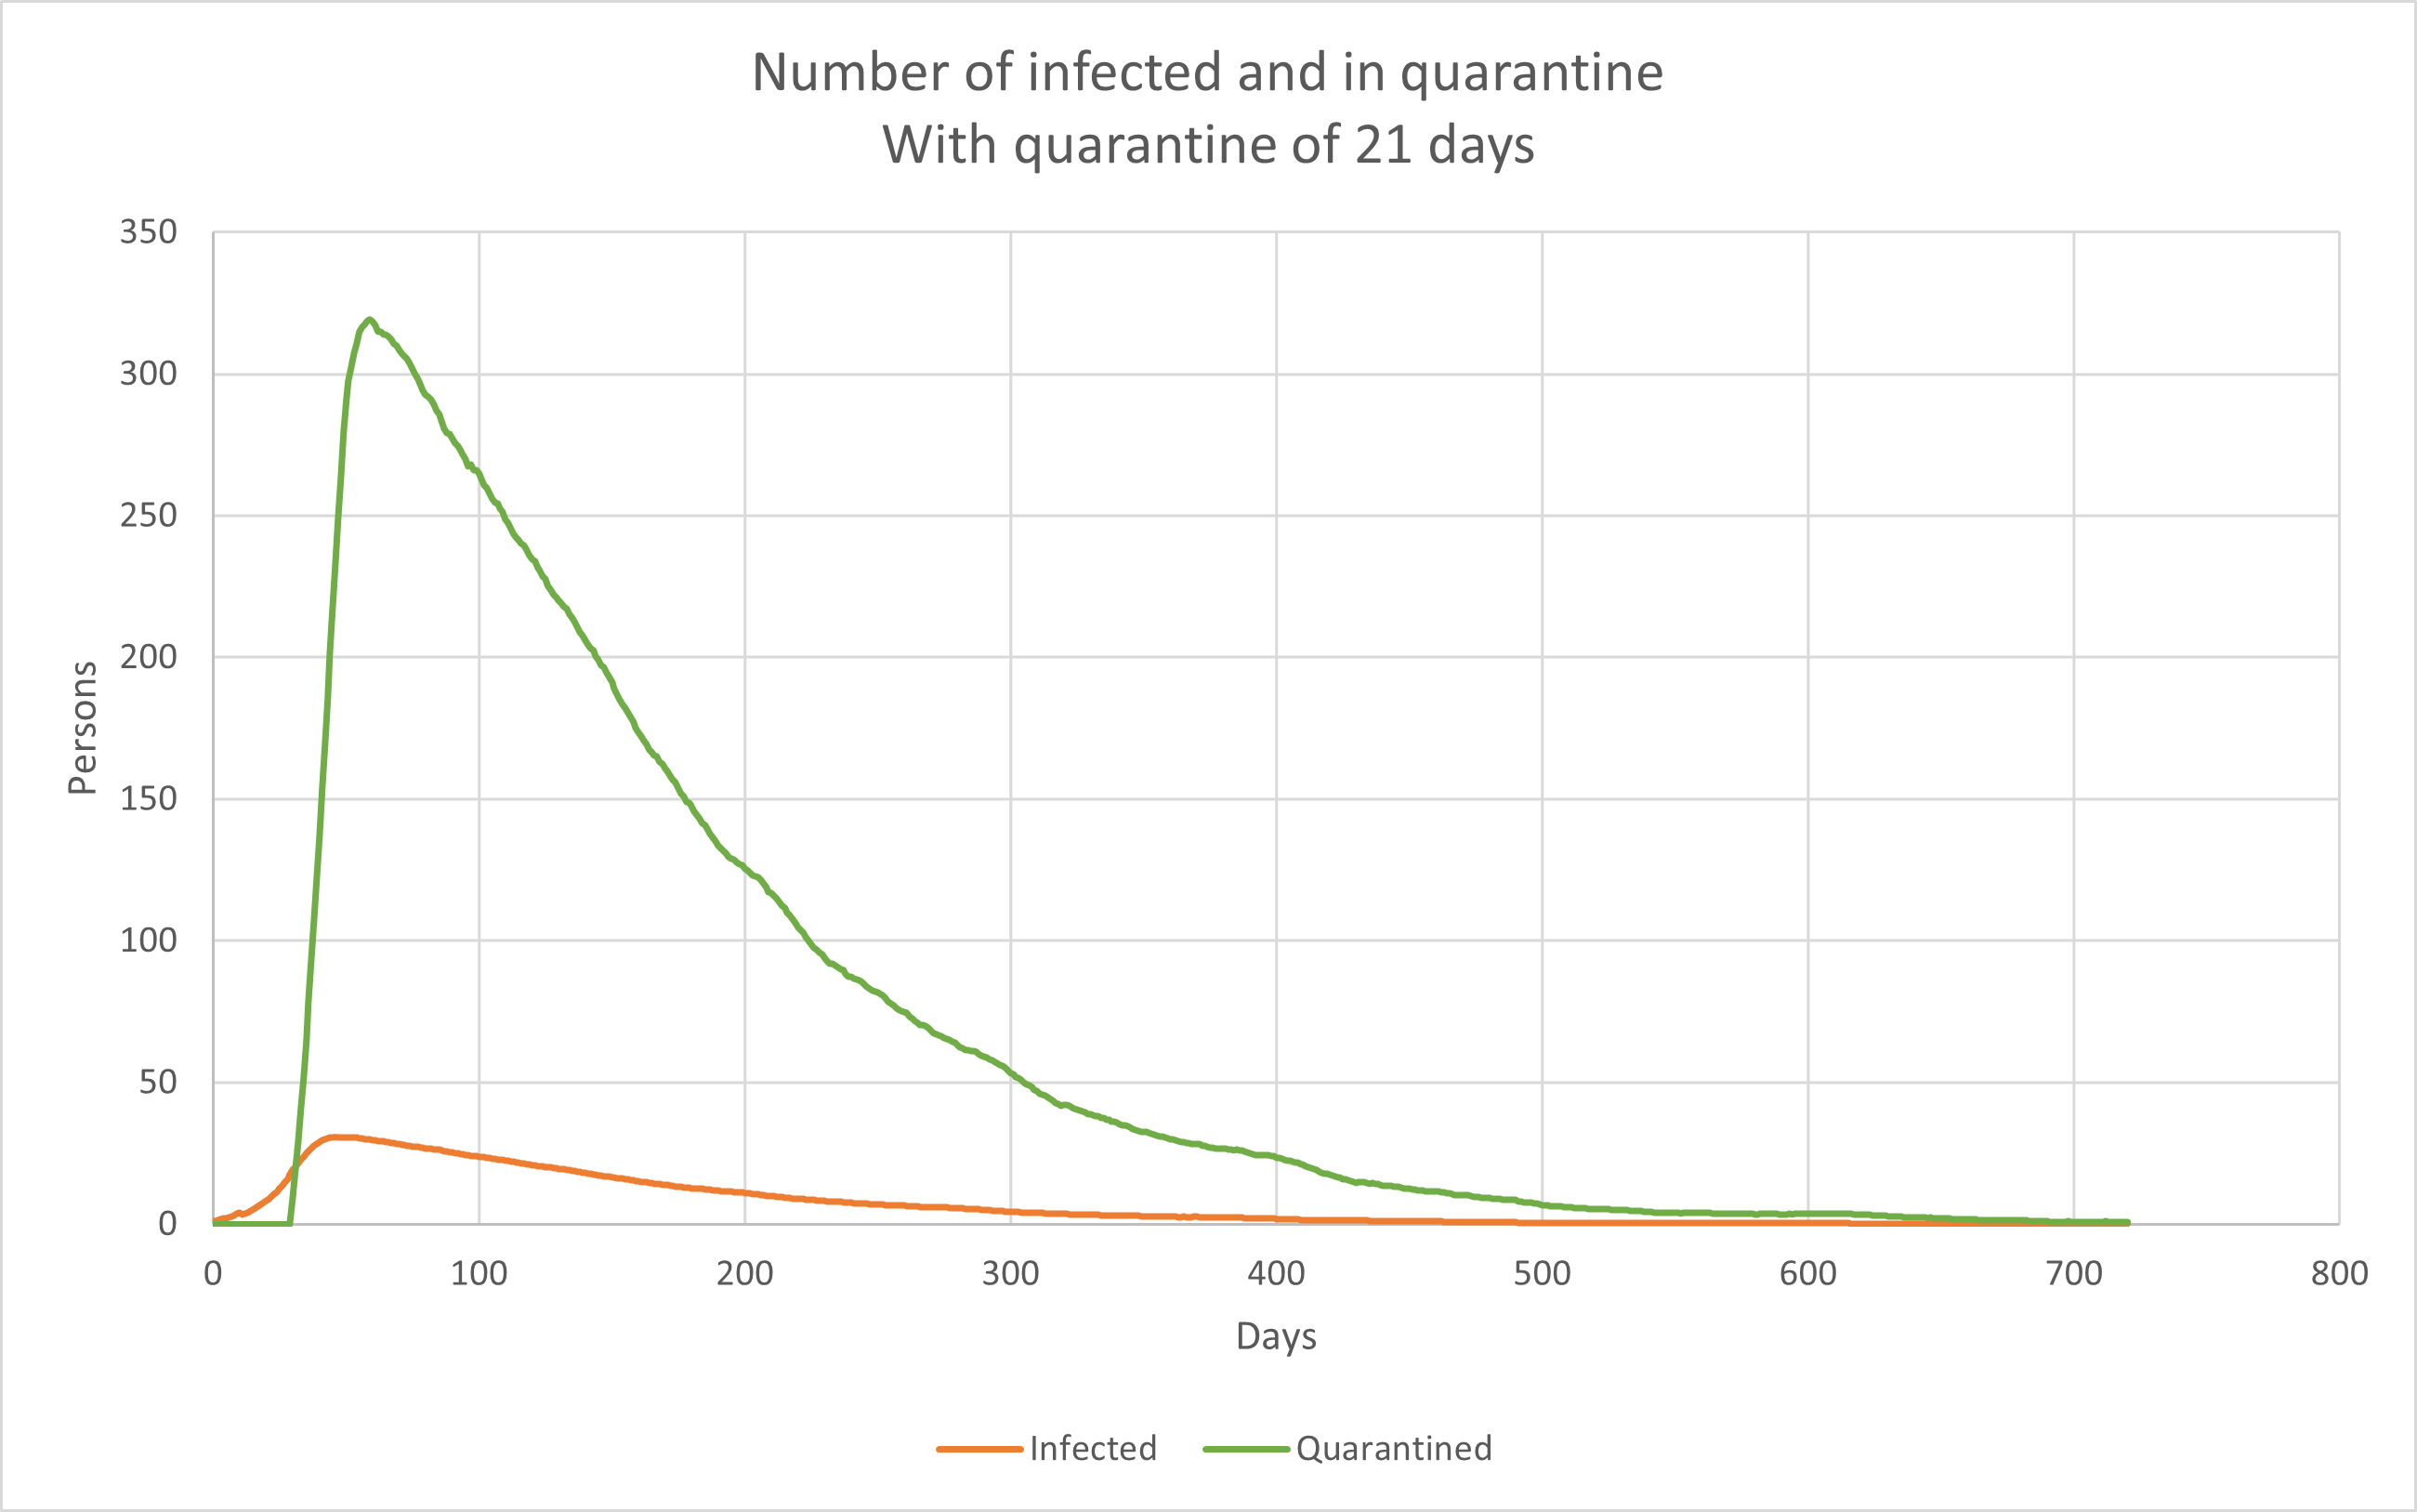
\includegraphics[width=.95\linewidth]{0_billeder/CT_Q_21.png}
  \caption{Quarantine period of 21 days}
  \label{fig:sub2}
\end{subfigure}
\caption{Comparison between 7 day and 21 day quarantine period}
\label{fig:test}
\end{figure}

The graphs show that when the quarantine period is increased, we see that we have a much lower number of infected people pr day




\begin{figure}[H]
\centering
\begin{subfigure}{.5\textwidth}
  \centering
  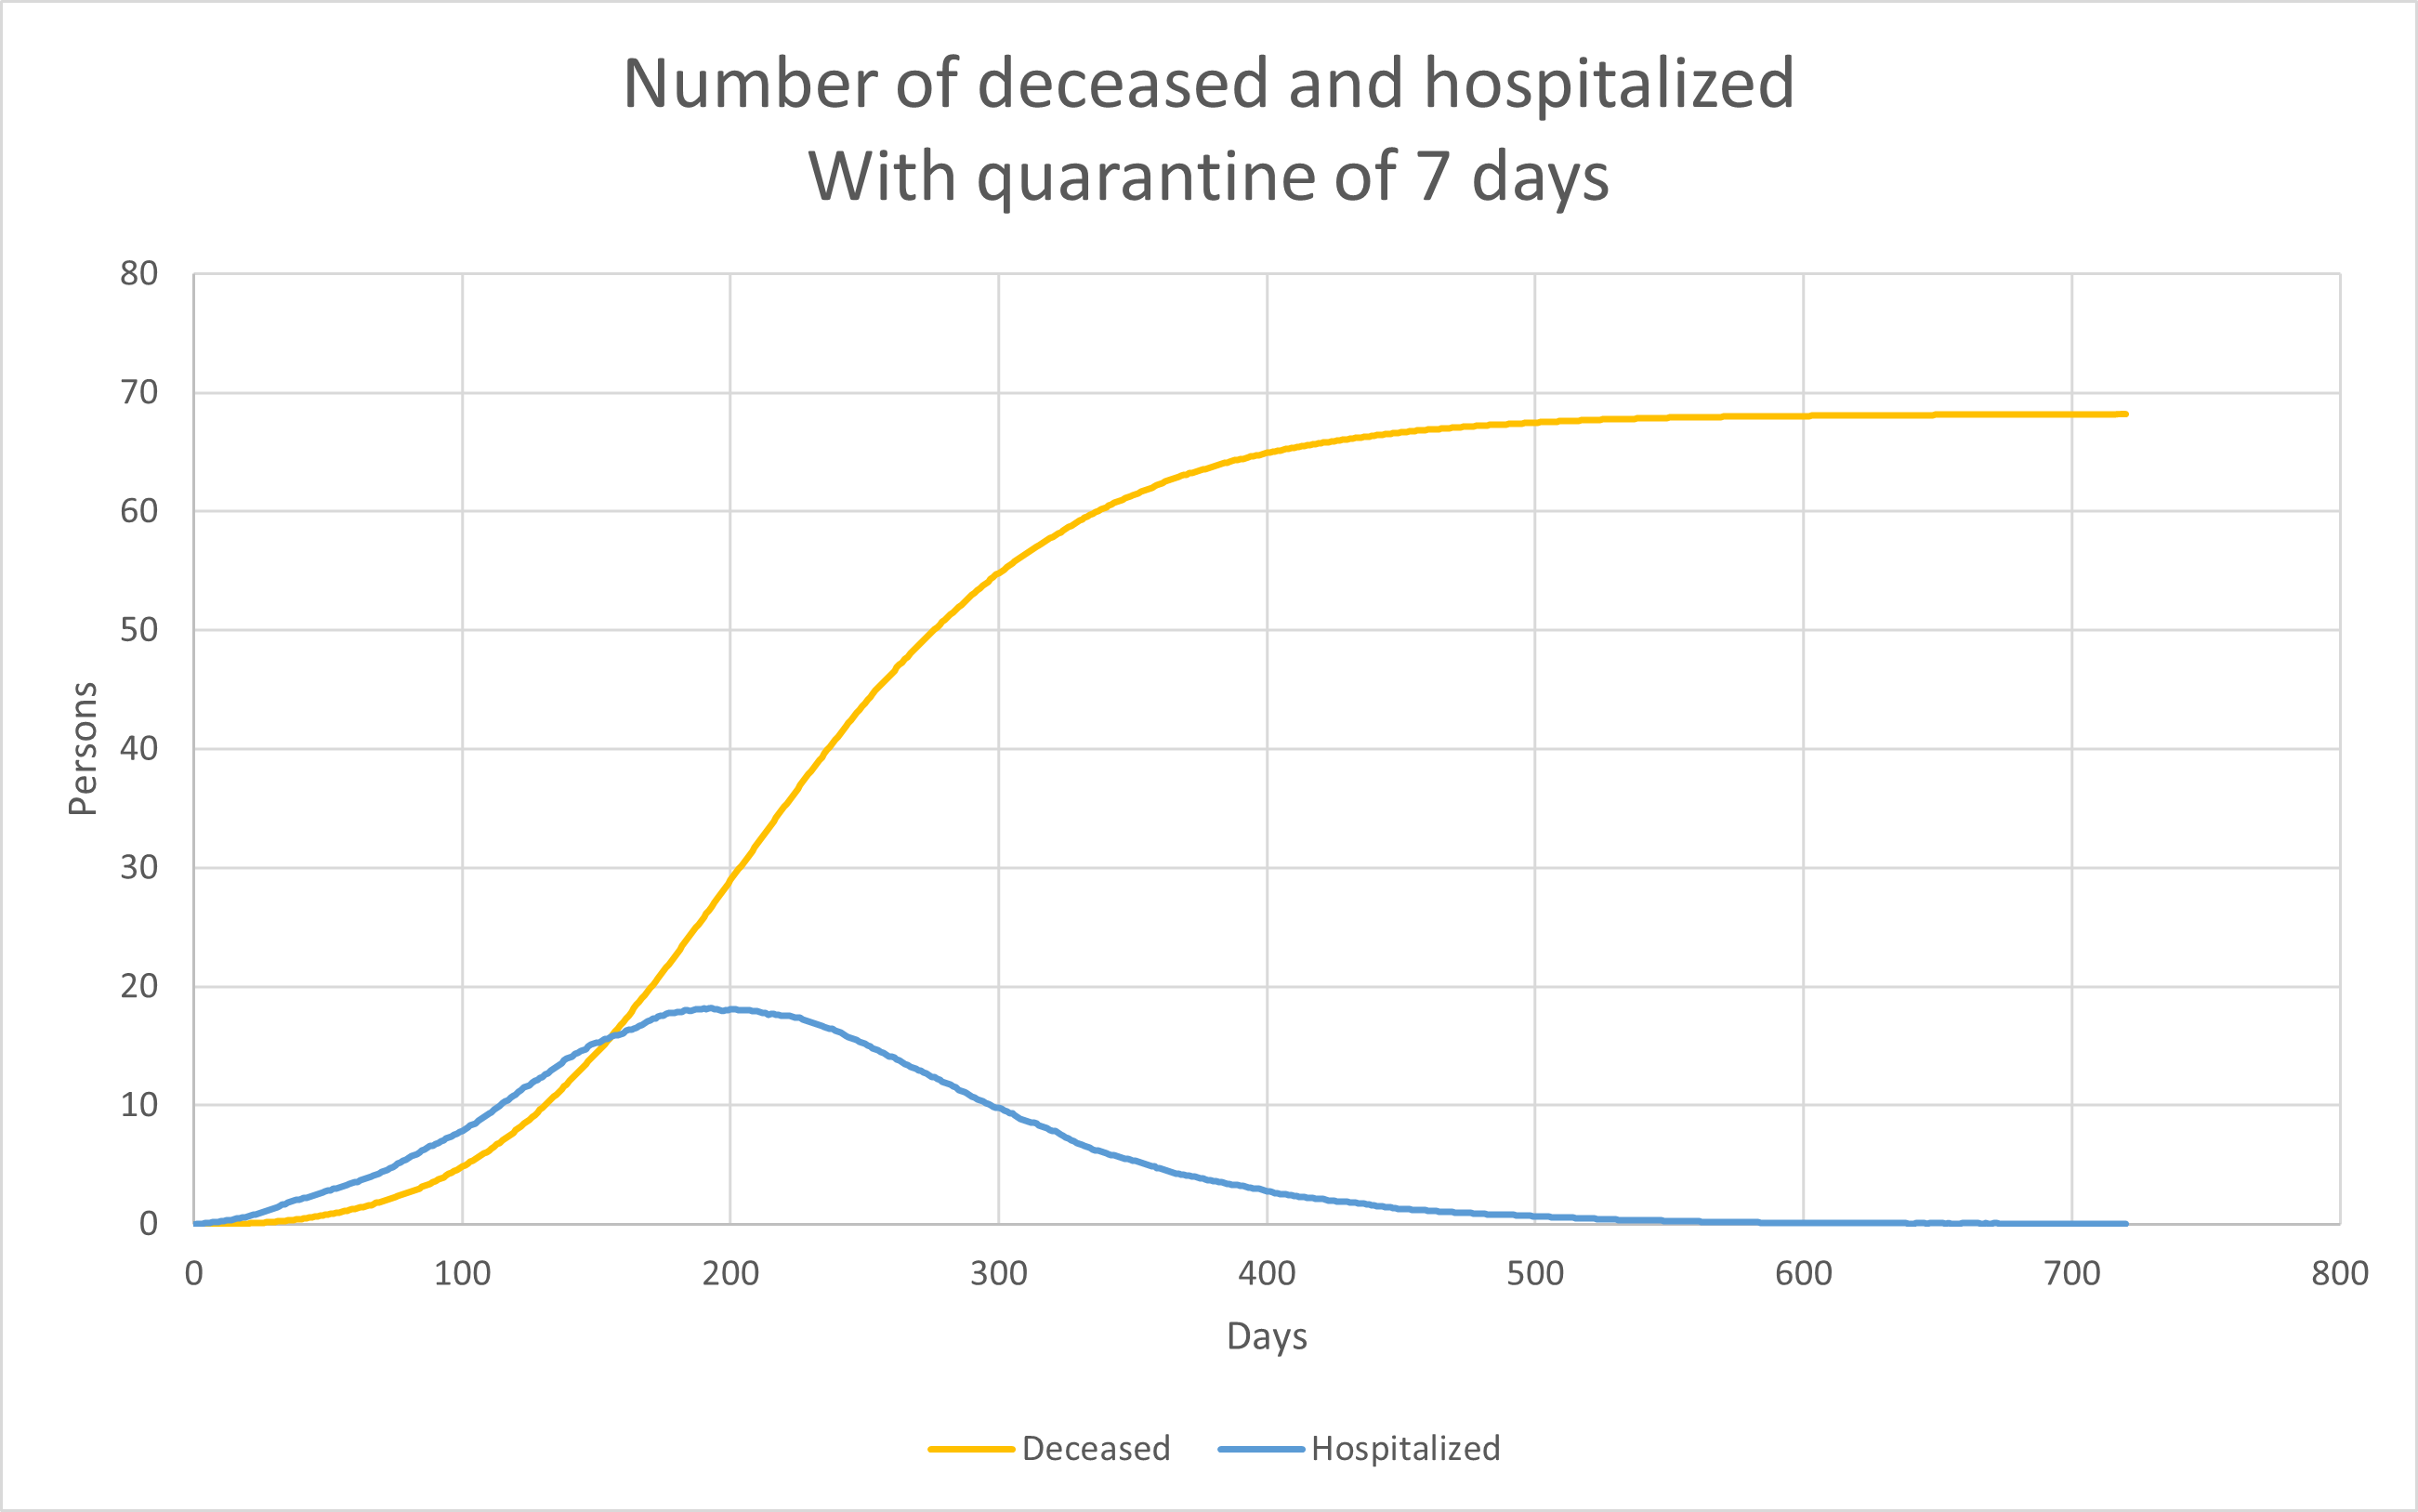
\includegraphics[width=.95\linewidth]{0_billeder/CT_HOS_7.png}
  \caption{Quarantine period of 7 days}
  \label{fig:sub1}
\end{subfigure}%
\begin{subfigure}{.5\textwidth}
  \centering
  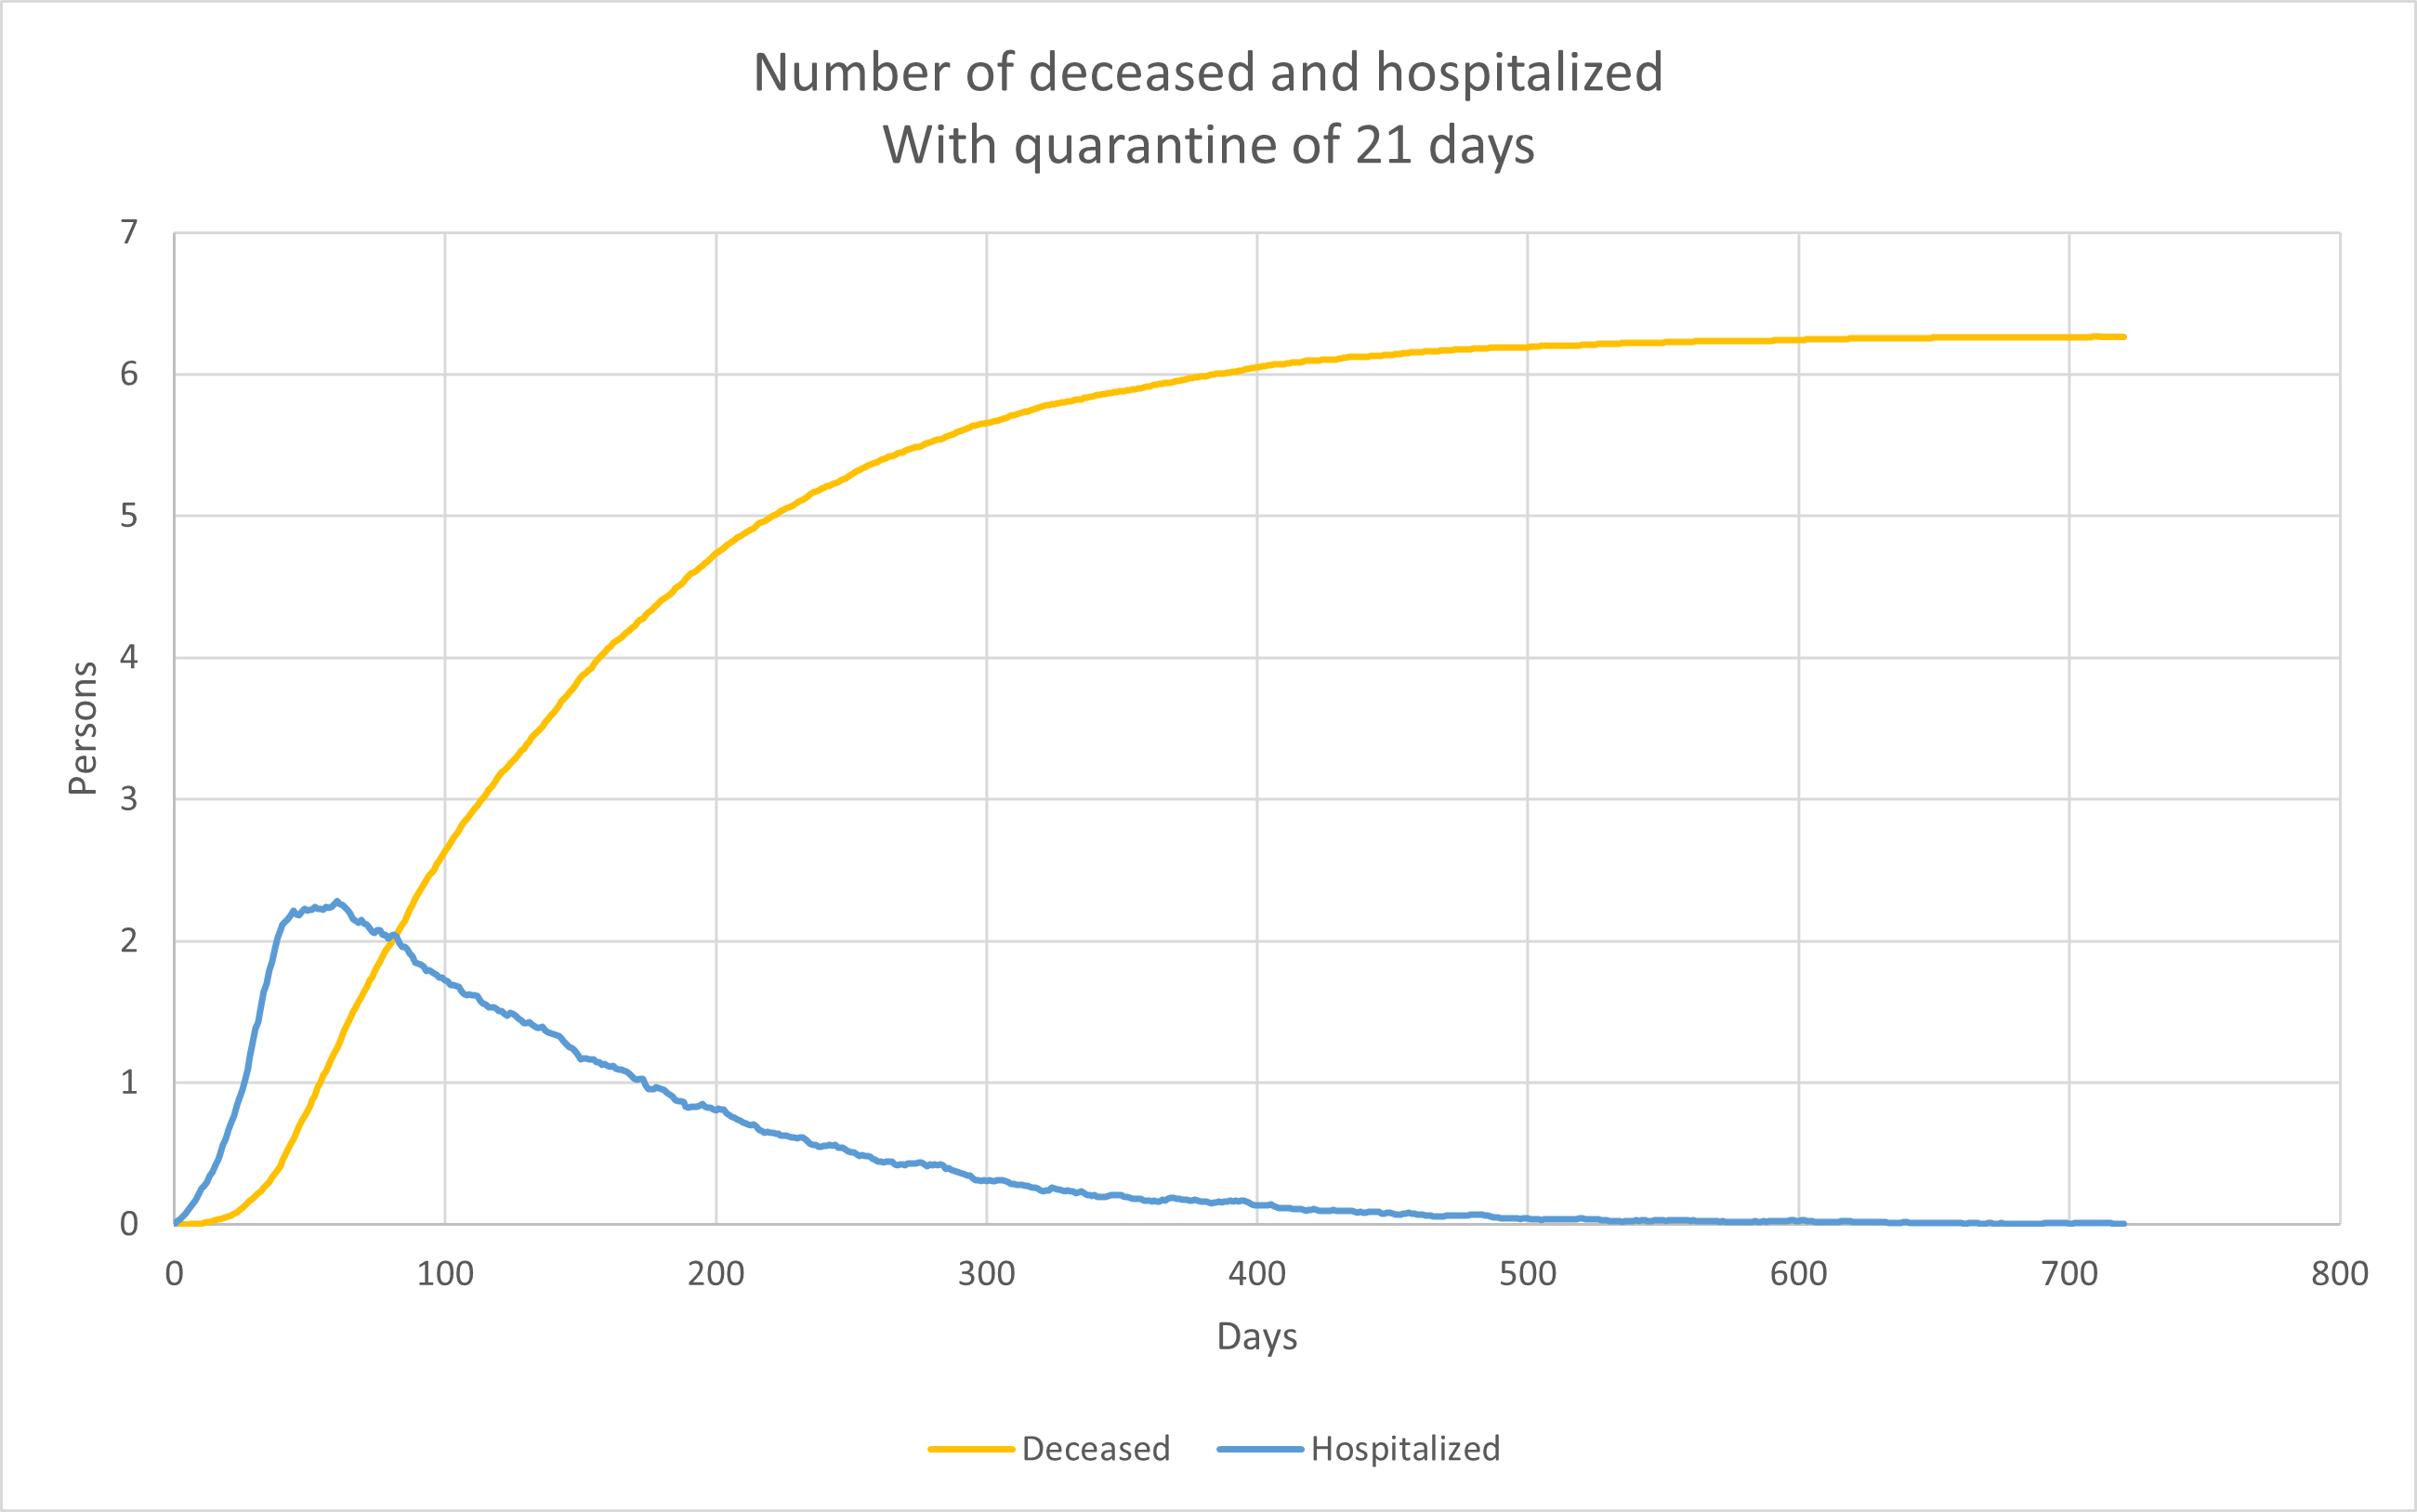
\includegraphics[width=.95\linewidth]{0_billeder/CT_HOS_21.png}
  \caption{Quarantine period of 21 days}
  \label{fig:sub2}
\end{subfigure}
\caption{Comparison between 7 day and 21 day quarantine period}
\label{fig:test}
\end{figure}


\subsection{Traceable contacts}


\subsection{COVID-19 and Its Effect on Hospital Capacity} \label{sub: Hospital Capacity}

A region's hospital capacity is in direct correlation with survival rates for the region's citizens. Therefore, having a hospital capacity that can withstand COVID-19 is vital for a society's ability to likewise withstand the pandemic. 

Since COVID-19 spread across the globe in early spring of 2020, each country's hospital capacity has been tested. Director of the Danish Health Authority, Søren Brostrøm, published a statement in March 2020 regarding nationwide strain on hospital capacity and a plan moving forward \citep{brostrom_notat_2020}. In this statement, he urged patients to minimise hospital visits and also gave examples of which operations can be postponed until Danish hospitals can move safely past COVID-19.

Some scholars have simulated hospital capacity on local scales, such as Weissman et al., whose aim is to predict hospital capacity needs within the greater area of Philadelphia, Pennsylvania, USA \citep{weissman_locally_2020}. Unfortunately, and as mentioned by Weissman et al., parameters for these types of simulations are typically taken from published data from heterogeneous sources. As stated in section \vref{sub: Statistical Uncertainty} in this report, this is also a limitation that we have encountered throughout data collection for our simulation.

Our proposal for analysing COVID-19's effect on hospital capacity is instead to see hospital capacity as a static number and compare this static value to the number of severely infected in our source code (see Appendix \ref{Appendix: SourceCode} Source Code). From the get-go, we have viewed our severely infected medical state as the medical state needing medical care.

\subsubsection{Definition of Hospital Capacity}

What is meant with the phrase \say{hospital capacity}? Each hospital has some influence on what is meant with this phrase, meaning that there is not a universal definition. However, all hospitals within the same country have. Because the scope of this project's simulation is limited to the greater Aalborg area, we will use a Danish definition of hospital capacity. This definition includes the following for each hospital:
\begin{itemize}
\item Available medical personnel
\item Available beds for patients
\item Available beds for patients within the Intensive Care Unit (ICU)
\item Available respirators for patients
\end{itemize}

If a hospital is reaching its capacity, patients can be moved to other hospitals. Therefore, while the individual hospital has its own capacity, the phrase \say{hospital capacity} can also refer to the entire nation's capacity.

For this project and simulation, which is based on a much smaller geographical scale, we will focus on the hospital capacity of Aalborg.

\subsubsection{Hospital Capacity in Denmark}

The hospital capacity within Denmark has steadily risen since the beginning of the COVID-19 pandemic in preparation for an aggravated increase in infected people. Specifically for Aalborg and Northern Jutland, a pandemic unit was established with 47 beds in total; 30 regular beds and 17 beds for intensive care \citep{dansk_sygeplejerad_fra_2020}. The number of respirators for each hospital remains unknown, but this information gives us a number to calculate with.

An important note to add on to this is the fact that hospitals can adapt relatively quickly to an increase in patients. As seen on esundhed.dk, the number of occupied beds in ICUs in Aalborg hospitals increased dramatically during March and April (\cite{esundheddk_sengepladser_2020}). March and April were the months throughout which the pandemic was at its first peak. Precise numbers were 32 beds in February, 78.8 in March, 90.9 in April and 51.3 in May. 

\subsubsection{Our Simulation's Hospital Capacity Results}

As with all other figures in chapter \ref{chap:result}: Results, the graphs on hospitalisation are based on the 808420 seed. As can be seen in figure \vref{fig:hospitalized NO CT}, hospitalisation peaks just about the same time as peak of infection (as seen in figure \vref{fig:peak_infected}). Infection peaks around day 112, whereas hospitalisation peaks around day 108. Since hospitalisation is dependent upon severe infection, the correlation is logical. The peak for hospitalisation is 200 people.

\begin{figure}[H]
  \centering
  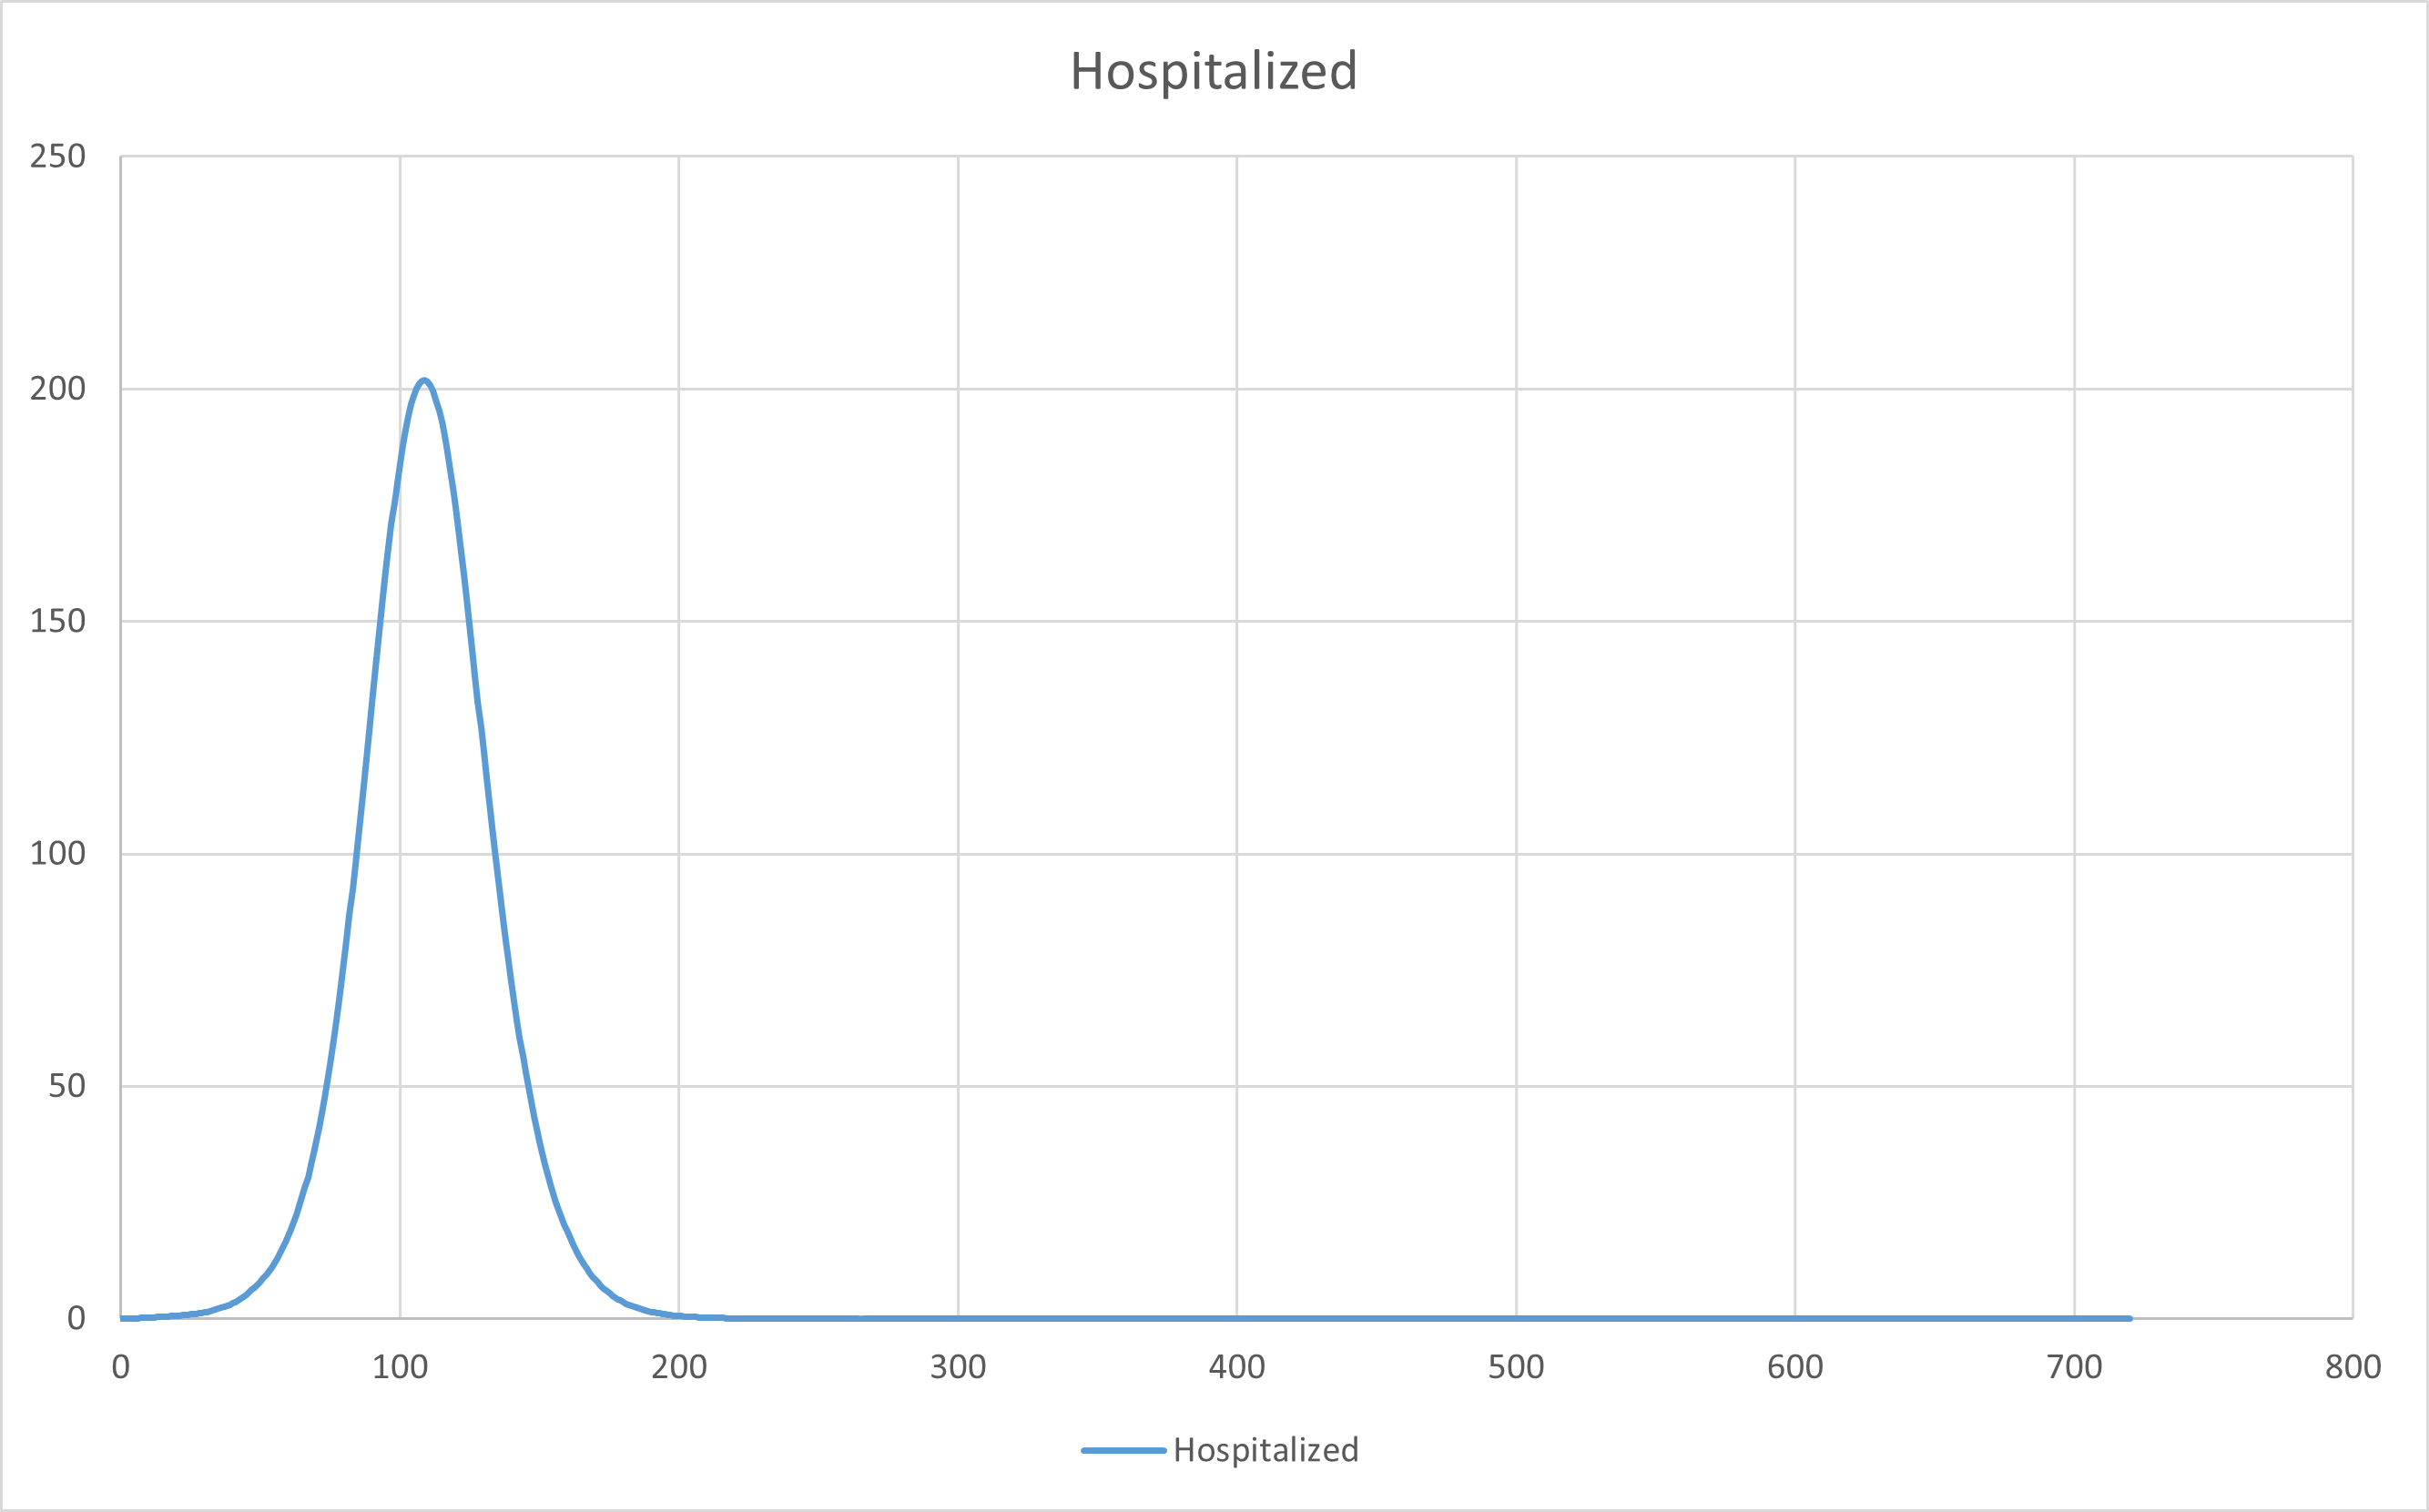
\includegraphics[width=140mm]{0_billeder/Hospitalized_no-CT.png}
  \caption{Hospitalised patients per day throughout the simulation with contact tracing disabled.}
  \label{fig:hospitalized NO CT}
\end{figure}

As previously stated, the hospital capacity for our entire population (Aalborg area) is 47 beds in total. Therefore, the hospital capacity for our simulation is greatly exceeded. Whether our simulation is seen as representative for the entire population of Denmark or comparative to similar simulations for the rest of Denmark, it can be inferred that this excess in hospitalised patients can be disastrous. Even if taking into account that Aalborg Universitetshospital allowed for 90.9 patients during the highest peak of the pandemic's first wave, there is still an excess of more than 100 percent.

While the infection relatively quickly dies off again in this simulation (under the assumption that re-infection and mutation are not possible), the human and economic cost of exceeding hospital capacity by this much would be quite large.

In comparison, the figure for hospitalisations in a simulation where contact tracing is enabled is quite different, as seen below.

\begin{figure}[H]
  \centering
  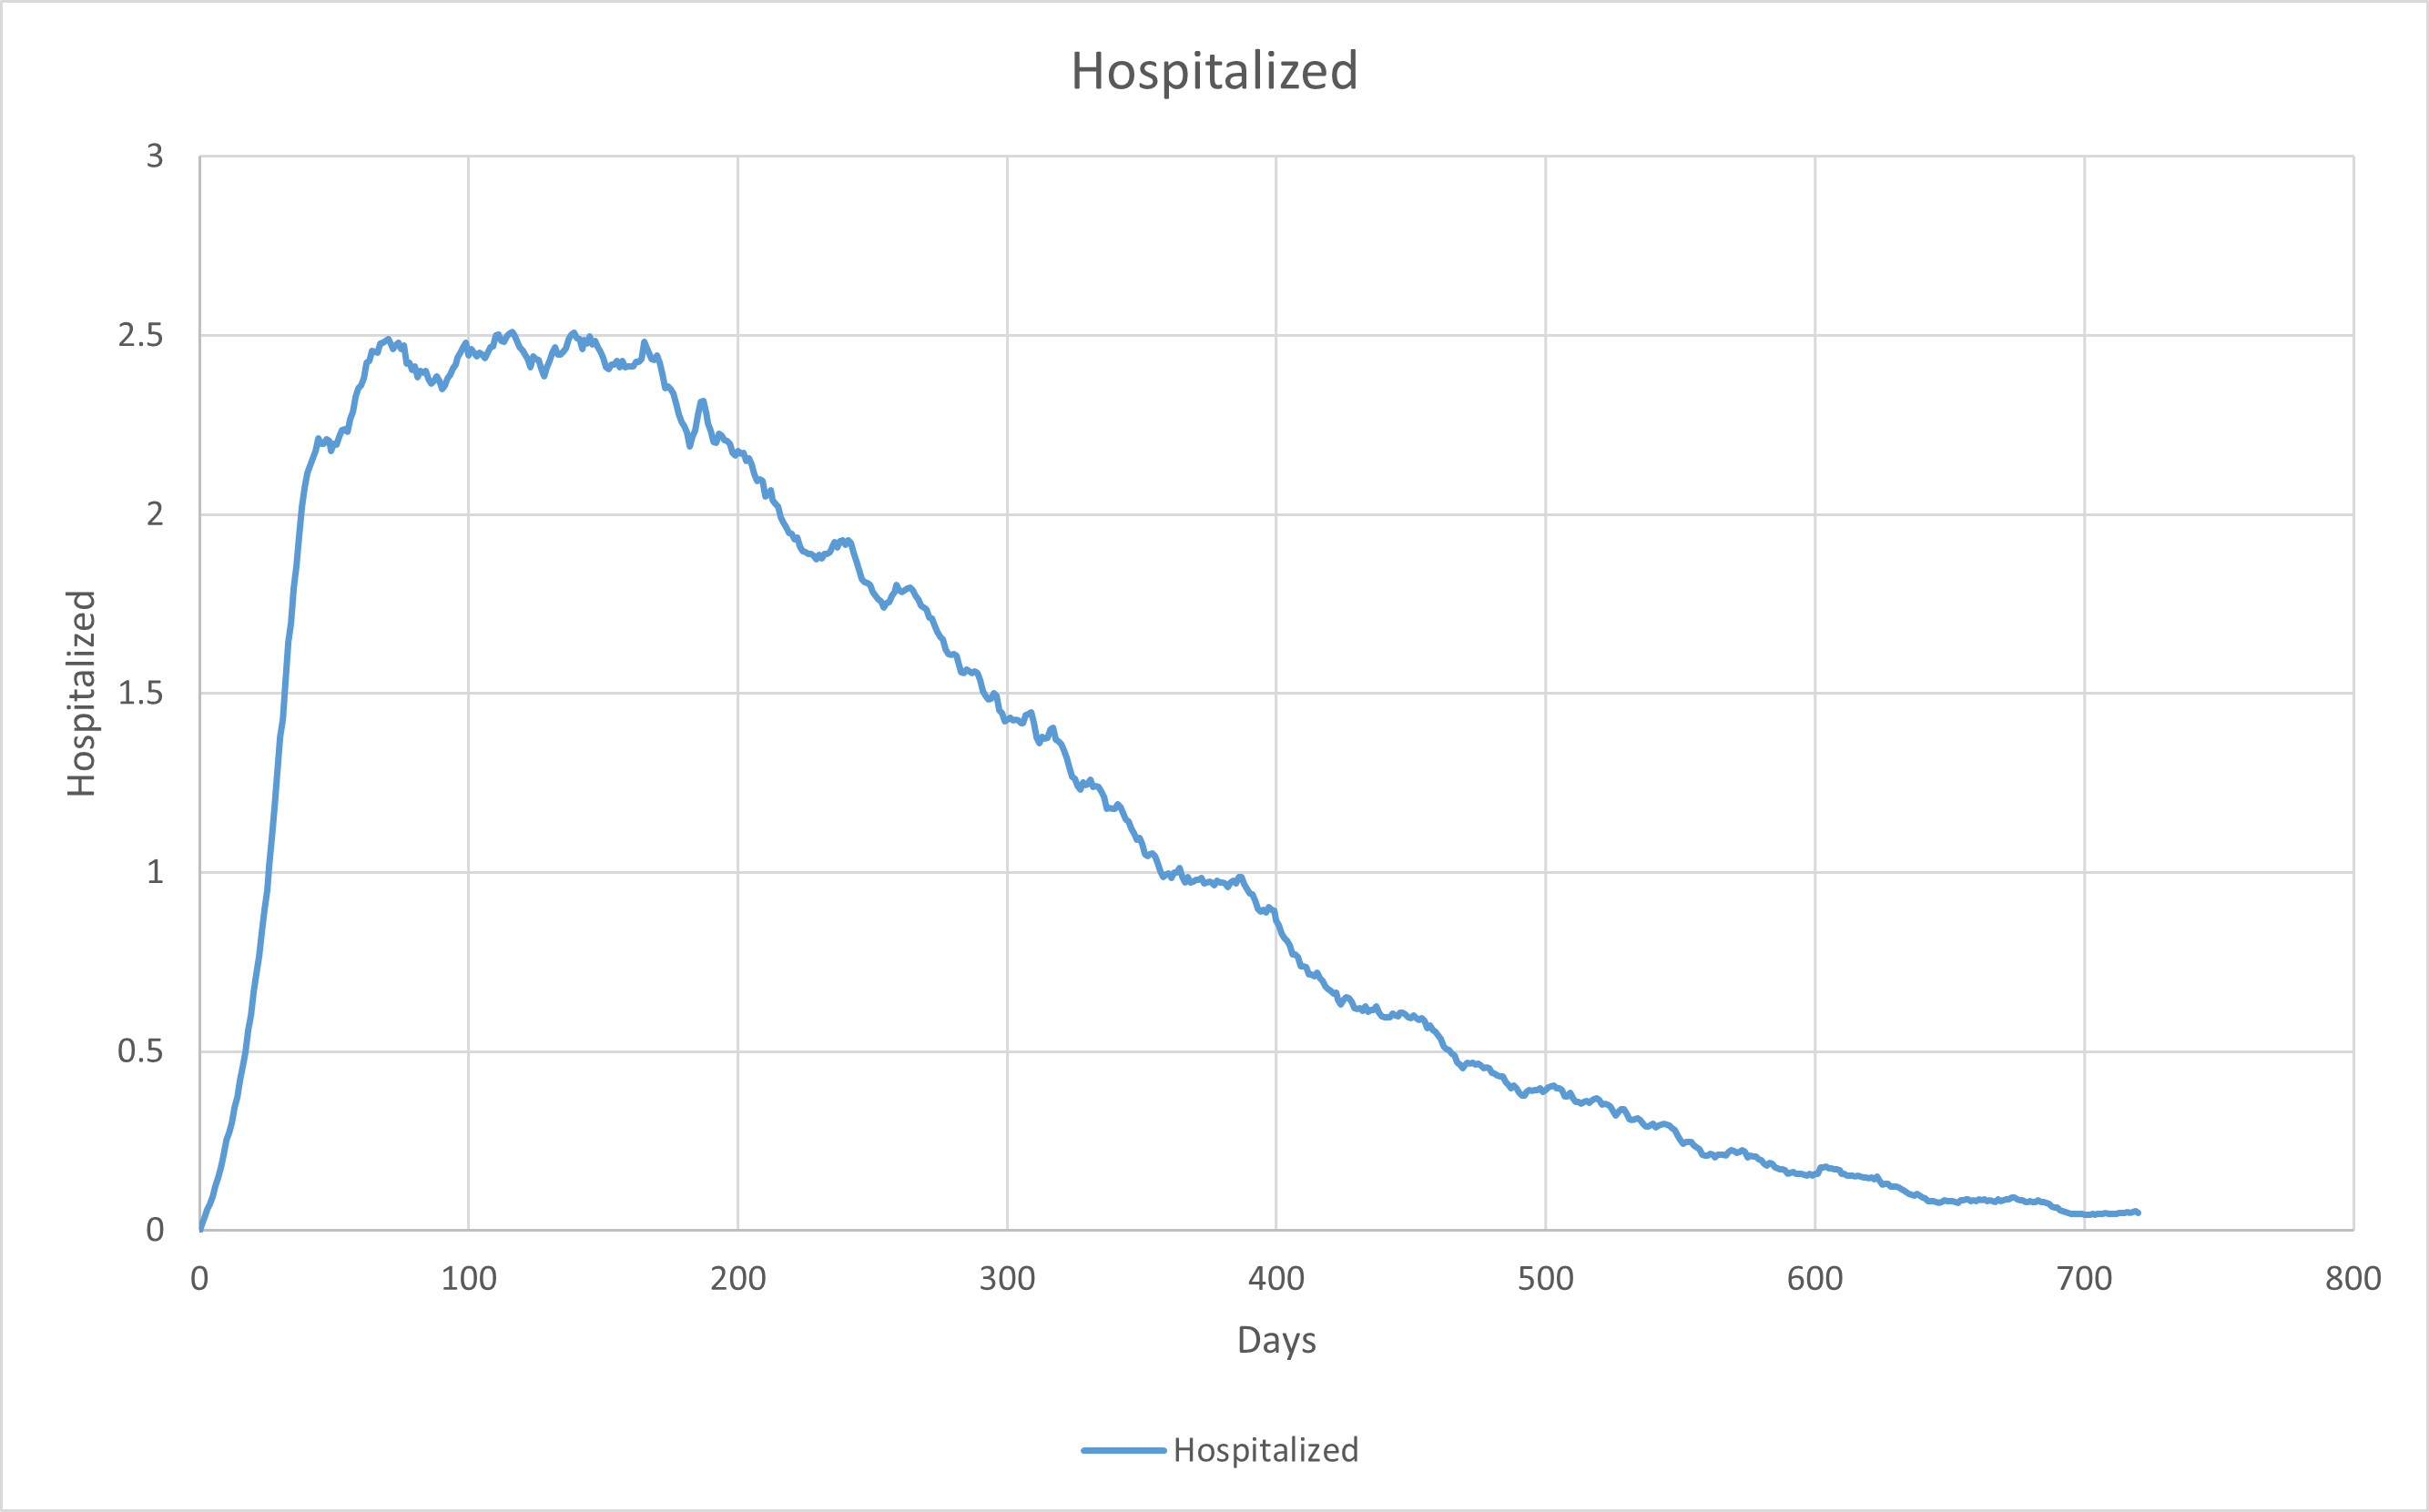
\includegraphics[width=140mm]{0_billeder/Hospitalized_WITH-CT.png}
  \caption{Hospitalised patients per day throughout the simulation with contact tracing enabled.}
  \label{fig:hospitalized WITH CT}
\end{figure}

As seen in figure \vref{fig:hospitalized WITH CT}, it takes considerably longer for the hospitalisations to die out compared to figure \vref{fig:hospitalized NO CT}. However, the number of hospitalisations is a fraction of the hospitalisations for the simulation with no contact tracing. Therefore, while hospitals will have to deal with infected patients for much longer, the human and economic cost of a pandemic where contact tracing is implemented is arguably lessened.

As shown in figure \vref{fig:hospitalized WITH CT}, the number peaks around day 90 and maintains this peak for almost 100 days. However, the peak is at 2.5 hospitalisations. Therefore, the hospital capacity for the population in our simulation is not remotely exceeded.

There are naturally more factors to consider. Since Denmark makes use of pandemic units that are completely closed off from the outside world (\cite{dansk_sygeplejerad_fra_2020}), risk of further infecting other civilians as well as medical personnel is likewise lessened.

\chapter{Conclusion} \label{chap:Konklusion}

%"" This technology has been effective in almost all disease outbreaks, and as a result of our project, once again contact tracing will prove very effective against outbreaks, both national and regional.  "" - SKAL KOMME EFTER RESULTATERNE, FOR AT BEKRÆFTE VORES TEORI, AT CT VIRKER.  


%Noter at de gennem
\chapter{Further Research} \label{chap:Further research}

\section{Updated Analysis}

%If you have updated information on statistics and so on which are not the ones you have based your analysis on, you can always comment on this in the future work section, describing what an updated version of the program should consider.

%In summary, if the more “correct” assumptions does not lead to major extra work, then you should go for it. Otherwise keep the “old” assumptions, and mention the new updated analysis as future work. I recommend to discuss this in the team and make your choice asap.

\section{Sex as a Factor}

%%%% Kilder %%%%
\begingroup
	\raggedright
	\bibliography{0_bibtex/Zotero-Group-refs.bib}							% Litteraturlisten inkluderes
    \label{litlist}                                             % Muliggoer at taelle sidetal
\endgroup

%%%% Fixme-listen %%%%
% \newpage														% Ny side til Fixme-listen
% \listoffixmes													% Fixme-listen - fjernes til sidst i projektet med "%"
% Basic commands: \fxnote, \fxwarning, \fxerror
% Fuld dokumentation af commands: https://www.lrde.epita.fr/~didier/software/fixme.pdf


%%%%%%%% Appendiks %%%%%%%%
\appendix
% Appendiks/bilag start - giver chapter bogstaver i stedet for tal
\clearforchapter												% Sikrer at pagestylen aktiveres paa den rigtige side
\phantomsection													% Kunstigt afsnit, som hyperlinks kan 'holde fast i'
\pdfbookmark[0]{Appendiks}{appendiks}							% Tildeler en klikbar bookmark til den endelige PDF

%% Indstillinger for appendiks (deaktiveret med "%") %%

\pagestyle{empty}												% Sidehoved/-fod for standardsider aendres til tom for appendiks
\aliaspagestyle{chapter}{empty}								    % Sidehoved/-fod for kapitelsider aendres til tom for appendiks
% \settocdepth{chapter}											% Kun kapitel-niveau vises i ToC
\addtocontents{toc}{\protect\cftpagenumbersoff{chapter}}		% Sidetal for kapitler fjernes i ToC

%% Filer til appendiks %%

% \include{appendiks/appendiks1}


%%%%%%%% Bilag %%%%%%%%
\addcontentsline{toc}{chapter}{Appendix}                           % Manuelle indgang til Bilag i indholdsfortegnelsen
\phantomsection												    % Kunstigt afsnit, som hyperlinks kan 'holde fast i'
\chapter{Source Code} \label{Appendix: SourceCode}

\begin{lstlisting}[language=c, caption={Our simulations written in c}, captionpos=b, label={snippet:LABELNAVN}]
#include <stdio.h>
#include <stdlib.h>
#include <string.h>
#include <stdbool.h>
#include <time.h>
#include <math.h>

/*Defines the size of the population, which will be used in the simulation
 - NOTE: population cant exceed RAND_MAX, since we use this for selection when infecting, 
 which means that only the people with index 0 to RAND_MAX in the population array can be selected*/
#define populationSize 12500

/*Seed used to seed the randomizer.
 - NOTE: time(0) can be used to generate a random number on runtime, but any int can be used*/
#define seed time(0)

/*Defines the number of contacts that a person has in a given day. 
- NOTE: It will not affect the infectionrate, but will affect the number of people quarantined if contact tracing is on*/
#define avgContacts 10

#define quarantinePeriod 14 /*Defines the time traced contacts will be quarantined*/
#define timeFrame 720       /*Timeframe is the number of days the simulation will run for*/
#define numOfDrops 100      /*The number of simulations that are run when the program starts*/

#define reproductiveNumber 2.5                               /*The reproductive number is the number of people an infected person infects on average.*/
#define avgInfectionPeriod 10                                /*Defines how long people will be infected for*/
#define incubationPeriod (rand() % 8 + 3)                    /*Defines how long people will be in incubation before they become sick and can infect others*/
#define asymptomaticPeriod (rand() % avgInfectionPeriod + 1) /*Defines how long the person will be asymptomatic -NOTE: This affects contact tracing*/

#define startInfectedAmount 1 /* Defines the amount of people to be infected on day 1 of the simulation*/

#define contactTracing true                                    /*Switch to false to turn off contact tracing*/
#define contactTracingStartTime 30                             /*Defines from what day the contact tracing begins in the simulation*/
#define traceableContacts (rand() % (avgContacts * 2 - 4) + 5) /* Defines how many contacts of an infected person that can be traced */

/*The different sex a person can be*/
enum sex
{
    female,
    male
};

/*The different states that a person can be in*/
enum states
{
    susceptible,
    infected,
    recovered,
    deceased
};

/*The different age-groups a person can be in*/
enum age
{
    underSixty,
    sixties,
    seventies,
    eighties,
    ninetyPlus,
};

/*Struct which contains all variables for each person in population */
struct Person
{
    int ID;
    int age;
    int sex;
    int state;
    int asymptomaticTimer; /*The asymptomatic timer is for asymptomatic patients as well as pre-symptomatic patients*/
    int incubationTimer;
    int infectionTimer;
    int quarantineTimer;
    int infectionPeriod;
    int numOfContacts;
    bool incubation, severelyInfected, quarantine;
    int contactID[avgContacts], tracingID[avgContacts * 2];
};

typedef struct Person Person;

/* Function Prototypes */
void UpdatePopulation(Person *population, int time);
void UpdateContacts(Person *population, int infectedID);
bool CheckContacts(Person infectedPerson, Person contact, int ID);
void SaveResultsToFile(FILE *file, int results[][7], int maxValueInDrop[][4]);
void SaveDrop(Person *population, int time, FILE *file, int drop, int selectedDrop);
void SaveResults(Person *population, int results[][7], int maxValueInDrop[][4], int drop, int time);
void ResetContacts(Person *population, int time);
void setAgeSex(Person *population);
int CountState(Person *population, int status);
int CountAge(Person *population, int ageGroup);

int main()
{
    printf("Simulating...\nResults are being generated: \n");
    int startInfection;
    int localSeed = seed;

    /* file pointer is initialized and a .csv file is generated to store the data from the simulation*/
    FILE *fPointer;
    char strSeed[40];
    sprintf(strSeed, "%i", localSeed);
    char *fileName = strcat(strSeed, "seed.csv");
    fPointer = fopen(fileName, "w");
    fprintf(fPointer, "seed:;%i;Number of drops:;%i\n\n\n", localSeed, numOfDrops);

    int resultArray[timeFrame][7] = {{0}}; /*Array which contains the sum of the results for all of the drops*/
    int maxValues[numOfDrops][4] = {{0}};  /*Array which contain all of the max values we are interested in extracting from each drop*/

    for (int drops = 1; drops <= numOfDrops; drops++)
    {
        /*We seed the randomizer for each drop, so that comparison is posibble, since if its not done, the next drops are affected by the previous drops rands*/
        srand(localSeed + drops);

        /*Dynamically allocate memory according to how big the population is. 
        --- WARNING --- Usage of static allocated arrays will result in not being able to use a population exceeding 12000*/
        Person *population = calloc(populationSize, sizeof(Person));

        /* Initializes all needed variables for the entire population*/
        for (int i = 0; i < populationSize; i++)
        {
            (population + i)->ID = i;
            (population + i)->infectionTimer = avgInfectionPeriod;
            (population + i)->incubationTimer = 7;
            (population + i)->infectionPeriod = avgInfectionPeriod;
            (population + i)->asymptomaticTimer = -1;
            (population + i)->state = susceptible;
            (population + i)->incubation = false;
            (population + i)->quarantine = false;
            (population + i)->quarantineTimer = quarantinePeriod;
            (population + i)->severelyInfected = false;
            (population + i)->numOfContacts = avgContacts - 1;

            /*All of the Contact IDs and Tracing IDs are initialized to -1, to be out of bounds for the population*/
            for (int j = 0; j < avgContacts; j++)
            {
                (population + i)->contactID[j] = -1;
            }
            for (int k = 0; k < avgContacts * 2; k++)
            {
                (population + i)->tracingID[k] = -1;
            }
        }

        /*Function call to set the age and sex distribution of the population*/
        setAgeSex(population);

        printf("%i ", drops);

        /* Infects the first people so the simulation can start*/
        for (int i = 0; i < startInfectedAmount; i++)
        {
            startInfection = rand() % populationSize;
            (population + startInfection)->state = infected;
            (population + startInfection)->asymptomaticTimer = asymptomaticPeriod;
        }

        /* For every day in the timeframe, we check for an update of the state for each person in the population*/
        for (int days = 1; days <= timeFrame; days++)
        {
            UpdatePopulation(population, days);
            ResetContacts(population, days);
            SaveResults(population, resultArray, maxValues, drops, days);
        }

        free(population); /*The allocated memory gets freed up after we're done using it*/
    }

    SaveResultsToFile(fPointer, resultArray, maxValues);
    fclose(fPointer); /*The file is closed and data is saved*/
    printf("\nThe simulation has finished, a data file has been created\n");
    return EXIT_SUCCESS;
}

/*Function which saves the sum of the results of all the drops in the result array, 
it also saves the max value for the number of infected and hospitalized in each drop in the max value array*/
void SaveResults(Person *population, int results[][7], int maxValueInDrop[][4], int drop, int time)
{

    /*Temporary array which stores the time, number of people in different states and som sub-states.
    Its used to load the values in the result array*/
    int tempResult[7] = {0};

    tempResult[0] = time;

    tempResult[1] = CountState(population, susceptible);
    tempResult[2] = CountState(population, infected);
    tempResult[3] = CountState(population, recovered);
    tempResult[4] = CountState(population, deceased);

    for (int index = 0; index < populationSize; index++)
    {
        if ((population + index)->quarantine == true)
        {
            tempResult[6]++;
        }
        if ((population + index)->severelyInfected == true)
        {
            tempResult[5]++;
        }
    }

    if (maxValueInDrop[drop - 1][1] < CountState(population, infected))
    {
        maxValueInDrop[drop - 1][0] = time;
        maxValueInDrop[drop - 1][1] = CountState(population, infected);
    }
    if (maxValueInDrop[drop - 1][3] < tempResult[5])
    {
        maxValueInDrop[drop - 1][2] = time;
        maxValueInDrop[drop - 1][3] = tempResult[5];
    }

    /*the results are added to the resul array*/
    results[time - 1][0] = tempResult[0];

    for (int i = 1; i < 7; i++)
    {
        results[time - 1][i] += tempResult[i];
    }
}

/* Updates the state of each person, this will be done accordingly to where they are in their incubation/infection period */
void UpdatePopulation(Person *population, int time)
{
    int tracingNum;

    /*Motality rate for the different age groups, these numbers were calculated from the official danish COVID-19 statistics on 09-12-2020.
    - NOTE: These numbers were calculated by the number of deceased in age groups devided by the number of hospitalized in the same age groups.
    This is because it is assumed in this simulation that the deceased were hospitalized before they died of the illness*/
    static double mortalityRateByAge[5] = {0.0132, 0.8923, 0.196, 0.3453, 0.7346};

    /* Checks through the entire population to see if the different checks or timers apply for each person*/
    for (int i = 0; i < populationSize; i++)
    {
        /*Checks if the individual fulfills the criteria for dying due to covid*/
        if ((population + i)->state != deceased && (population + i)->severelyInfected == true && (population + i)->incubation == false &&
            ((double)rand() / (double)RAND_MAX) <= mortalityRateByAge[(population + i)->age] / avgInfectionPeriod)
        {
            (population + i)->state = deceased;
            (population + i)->asymptomaticTimer = -1;
            (population + i)->infectionTimer = -1;
            (population + i)->severelyInfected = false;
        }
        /* Makes sure that the incubation timer ticks down if a person is in incubation*/
        if ((population + i)->incubation == true)
        {
            (population + i)->incubationTimer--;

            /* Makes sure that a person is taken out of incubation if incubation timer reaches 0*/
            if ((population + i)->incubationTimer == 0)
            {
                (population + i)->incubation = false;
                (population + i)->incubationTimer = -1;
            }
        }

        /* Makes sure that the quarantine timer ticks down if a person is in quarantine*/
        if ((population + i)->quarantine == true)
        {
            (population + i)->quarantineTimer--;

            /* Makes sure that a person is taken out of quarantine if the quarantine timer reaches 0*/
            if ((population + i)->quarantineTimer == 0)
            {
                (population + i)->quarantine = false;
                (population + i)->quarantineTimer = quarantinePeriod;
            }
        }

        /* Makes sure that a person get the state recovered if their infection timer reaches 0*/
        if ((population + i)->infectionTimer == 0)
        {
            (population + i)->state = recovered;
            (population + i)->severelyInfected = false;
            (population + i)->infectionTimer = -1;
        }
        /* Makes sure that if a person gets covid symptoms they get put in quarantine and their tracable contacts 
           gets traces and put in quarantine aswell*/
        tracingNum = traceableContacts;

        if ((population + i)->asymptomaticTimer == 0 && (population + i)->state == infected &&
            (population + i)->quarantine == false && contactTracing == true && time >= contactTracingStartTime)
        {
            (population + i)->quarantine = true;

            for (int j = 0; j < tracingNum; j++)
            {
                if ((population + i)->tracingID[j] >= 0)
                {
                    (population + (population + i)->tracingID[j])->quarantine = true;
                }
            }
        }

        /* Makes sure that if the asymptomatic timer reaches 0, the person is no longer symptomatic. 
        Setting the timer to -1 ensures that they as well as their contacts dont end up in quarantine multiple times because of contact tracing*/
        if ((population + i)->asymptomaticTimer == 0)
        {
            (population + i)->asymptomaticTimer = -1;
        }
        /* If a person is infected and able to infect others, their contacts are updated*/
        if ((population + i)->state == infected && (population + i)->incubation == false && (population + i)->quarantine == false)
        {
            UpdateContacts(population, i);
        }
        /* If a person is infected at is out of incubation period, their asymptomatic timer and infection timer is ticked down*/
        if ((population + i)->state == infected && (population + i)->incubation == false)
        {
            (population + i)->infectionTimer--;
            (population + i)->asymptomaticTimer--;
        }
    }
}

/* Genereates the contacts for the infected, and chooses whether the contact will be infected or not */
void UpdateContacts(Person *population, int infectedID)
{
    /* The used variables are defined*/
    static double severityAgeFactor[5] = {0.0266, 0.1255, 0.28874, 0.4707, 0.41935};
    double infectionChance;
    int contact;
    int neededContacts = (population + infectedID)->numOfContacts;

    /* Goes through every contact that the infected has*/
    for (int i = 0; i < neededContacts; i++)
    {
        /* Picks a random contact for the person as long as they haven't gotten number of contacts they need already.
        This loop also makes sure the contact is valid(i.e. not in quarantine, deceased, etc.)*/
        do
        {
            contact = (rand() % populationSize);
        } while (CheckContacts(*(population + infectedID), *(population + contact), contact));

        /* Sets the infected person as a contact of the contact and counts down their number of contacts*/
        (population + contact)->contactID[(population + contact)->numOfContacts] = (population + infectedID)->ID;
        (population + contact)->numOfContacts--;

        /* Sets the contact as a contact of the infected person and counts down their number of contacts*/
        (population + infectedID)->contactID[(population + infectedID)->numOfContacts] = (population + contact)->ID;
        (population + infectedID)->numOfContacts--;

        /* Sets a chance of infection*/
        infectionChance = (double)rand() / (double)RAND_MAX;

        /* Checks if the contact will get infected*/
        if (infectionChance < (reproductiveNumber / avgContacts / (population + infectedID)->infectionPeriod))
        {
            /* IF the contact is susceptible they will get infected*/
            if ((population + contact)->state == susceptible)
            {
                (population + contact)->state = infected;
                (population + contact)->incubation = true;
                (population + contact)->incubationTimer = incubationPeriod;
                (population + contact)->asymptomaticTimer = asymptomaticPeriod;

                /* Checks if the contact will get severely infected*/
                if ((double)rand() / (double)RAND_MAX <= severityAgeFactor[(population + contact)->age])
                {
                    (population + contact)->severelyInfected = true;
                    (population + contact)->asymptomaticTimer = 2; /*assumption that severe infections have a short asymptomatic period.*/
                }
            }
            else /* If the contact doesn't get infected, the check shall then continue to the next contact*/
            {
                continue;
            }
        }
    }
}

/* Function that takes in the results of the simulation prints it in the file*/
void SaveResultsToFile(FILE *file, int results[][7], int maxValueInDrop[][4])
{
    fprintf(file, "Drop nr.;Day;Max infected in drop;;Day;Max hospitalized in drop\n");

    for (int j = 0; j < numOfDrops; j++)
    {
        fprintf(file, "%i;", j + 1);
        fprintf(file, "%i;", maxValueInDrop[j][0]);
        fprintf(file, "%i;;", maxValueInDrop[j][1]);
        fprintf(file, "%i;", maxValueInDrop[j][2]);
        fprintf(file, "%i\n", maxValueInDrop[j][3]);
    }

    fprintf(file, "\n\n\n");

    fprintf(file, "Time;Susceptible;Infected;Recovered;Deceased;Hospitalized;Quarantined\n");
    fprintf(file, "0;%i;%i;0;0;0;0\n", populationSize - startInfectedAmount, startInfectedAmount);
    for (int i = 0; i < timeFrame; i++)
    {
        /*The result array is the sum of all the numbers from all of the drops on all days. This prints the average for each result for all of the days*/
        fprintf(file, "%i;%lf;%lf;%lf;%lf;%lf;%lf\n", results[i][0], ((double)(results[i][1] / (double)numOfDrops)), (((double)results[i][2] / (double)numOfDrops)),
                (((double)results[i][3] / (double)numOfDrops)), (((double)results[i][4] / (double)numOfDrops)), (((double)results[i][5] / (double)numOfDrops)),
                (((double)results[i][6] / (double)numOfDrops)));
    }
}

/* Bool function to assure that the infected's selected contact is valid*/
bool CheckContacts(Person infectedPerson, Person contact, int ID)
{
    for (int i = 0; i < avgContacts; i++)
    {
        if (infectedPerson.contactID[i] == ID || infectedPerson.numOfContacts < 0 || contact.numOfContacts < 0 ||
            infectedPerson.ID == ID || contact.quarantine == true || contact.state == deceased)
        {
            return true; /*Returns true, means that a new contact needs to be found*/
        }
    }
    return false; /*Returns false, means that the checked contact meets all of the criteria for being selected*/
}

/* Function that counts the amount of people in each state*/
int CountState(Person *population, int status)
{
    int i = 0;
    for (int j = 0; j < populationSize; j++)
    {
        if ((population + j)->state == status)
        {
            i++;
        }
    }
    return i;
}

/* Function that resets the contact array and puts old contact id's into the tracing array*/
void ResetContacts(Person *population, int time)
{
    for (int i = 0; i < populationSize; i++)
    {
        for (int k = 0; k < avgContacts; k++)
        {
            if (time % 2 == 0)
            {
                (population + i)->tracingID[k] = (population + i)->contactID[k];
            }
            else
            {
                (population + i)->tracingID[k + avgContacts] = (population + i)->contactID[k];
            }
        }

        (population + i)->numOfContacts = avgContacts - 1;
        for (int j = 0; j < avgContacts; j++)
        {
            (population + i)->contactID[j] = -1;
        }
    }
}

/*Age set per person, dependent on sex.*/
void setAgeSex(Person *population)
{
    /*Establishes the percentage of males in different age groups*/
    double underSixtyPercentageMale = 0.3751;
    double sixtiesPercentageMale = 0.0573;
    double seventeesPercentageMale = 0.0457;
    double eigthiesPercentageMale = 0.0157;
    double ninetyPlusPercentageMale = 0.0024;

    double totalMales = underSixtyPercentageMale + sixtiesPercentageMale + seventeesPercentageMale + eigthiesPercentageMale + ninetyPlusPercentageMale;

    /*Defines to establish the percentage of females in different age groups
 - NOTE: that ninetyPlus for females is not needed since they make up the remaining part of population*/
    double underSixtyPercentageFemale = 0.3664;
    double sixtiesPercentageFemale = 0.0584;
    double seventeesPercentageFemale = 0.0505;
    double eigthiesPercentageFemale = 0.0225;

    /*For males*/
    for (int m = 0; m < ceil(populationSize * totalMales); m++)
    {
        (population + m)->sex = male;

        if (m < ceil(populationSize * (underSixtyPercentageMale)))
        {
            (population + m)->age = underSixty;
        }
        else if (m < ceil(populationSize * (underSixtyPercentageMale + sixtiesPercentageMale)))
        {
            (population + m)->age = sixties;
        }
        else if (m < ceil(populationSize * (underSixtyPercentageMale + sixtiesPercentageMale + seventeesPercentageMale)))
        {
            (population + m)->age = seventies;
        }
        else if (m < ceil(populationSize * (underSixtyPercentageMale + sixtiesPercentageMale + seventeesPercentageMale + eigthiesPercentageMale)))
        {
            (population + m)->age = eighties;
        }
        else if (m < ceil(populationSize * (totalMales)))
        {
            (population + m)->age = ninetyPlus;
        }
    }

    /*For females*/
    for (int f = ceil(populationSize * totalMales) + 1; f < populationSize; f++)
    {
        (population + f)->sex = female;

        if (f < ceil(populationSize * totalMales) + floor(populationSize * underSixtyPercentageFemale))
        {
            (population + f)->age = underSixty;
        }
        else if (f < ceil(populationSize * totalMales) + floor(populationSize * (underSixtyPercentageFemale + sixtiesPercentageFemale)))
        {
            (population + f)->age = sixties;
        }
        else if (f < ceil(populationSize * totalMales) + floor(populationSize * (underSixtyPercentageFemale + sixtiesPercentageFemale + seventeesPercentageFemale)))
        {
            (population + f)->age = seventies;
        }
        else if (f < ceil(populationSize * totalMales) + floor(populationSize * (underSixtyPercentageFemale + sixtiesPercentageFemale + seventeesPercentageFemale + eigthiesPercentageFemale)))
        {
            (population + f)->age = eighties;
        }
        else if (f < populationSize)
        {
            (population + f)->age = ninetyPlus;
        }
    }
}

/* Function that counts the amount of people in each agegroup*/
int CountAge(Person *population, int ageGroup)
{
    int i = 0;
    for (int j = 0; j < populationSize; j++)
    {
        if ((population + j)->age == ageGroup)
        {
            i++;
        }
    }
    return i;
}

/*Function which can save an individual drop to that data file, in case further analysis of a specific drop is neccesary*/
void SaveDrop(Person *population, int time, FILE *file, int drop, int selectedDrop)
{
    int q = 0, a = 0, s = 0;
    if (drop == selectedDrop)
    {
        for (int index = 0; index < populationSize; index++)
        {
            if ((population + index)->quarantine == true)
            {
                q++;
            }
            if ((population + index)->severelyInfected == true)
            {
                s++;
            }
            if ((population + index)->asymptomaticTimer >= 0)
            {
                a++;
            }
        }
        fprintf(file, "%i;%i;%i;%i;%i;%i;%i;%i\n", time, CountState(population, susceptible), CountState(population, infected),
                CountState(population, recovered), CountState(population, deceased), s, q, a);
    }
}
\end{lstlisting}

\chapter{First edition of flowchart} \label{Appendix:FirstFlowchart}

\chapter{Project Catalogue} \label{P1Katalog}
%\cftaddtitleline{toc}{section}{Bilag B: \ Projektkatalog}{} % Tilføj bilag til ToC manuelt

\includepdf[pages={7}]{0_appendiks/p1-katalog-e20.pdf}


\chapter{Data} \label{Appendix:Data}

The link leads to a google docs folder containing all the raw data from out simulation.
\url{https://drive.google.com/drive/folders/1JR-KBVjndgem9pnmJT2IZ2yq9nUzUli0?usp=sharing}

% Skabelon (Udkommenter med Ctrl+')
% \section*{Bilag B: bilagNavn}
% \addcontentsline{toc}{section}{Bilag B: \ bilagNavn} % Tilføj bilag til ToC manuelt
% \input{0_appendiks/bilagNavn.tex}



% Manuelle indgange i indholdsfortegnelsen (naar \includepdf bruges)			% Inkluder eksterne bilag med \includepdf[pages={x-y}]{filnavn}

\end{document}													% Slutter dokumentet - obligatorisk